\chapter[\uppercase{Static analysis of quantitative
noninterference}]{\uppercase{Static analysis of quantitative
noninterference}\protect\footnote{This chapter is excerpted from
previously published work~\cite{sscf} coauthored with Ziyun Qian,
Michael K. Reiter, and Yinqian Zhang.}}
\graphicspath{{./}{./fig/sscf/}{./fig/sscf/}{./fig/sscf/models/}}
\label{chap:sscf}
The quantitative noninterference evaluation for cache mitigation in
the previous \chapref{chap:cachebar} is attack-specific. In this
chapter, we propose a static method to measure interference in
software using static analysis before it happens. 

Our intuition draws from
\textit{noninterference}~\cite{goguen1982security}, which informally
is achieved when the attacker-controlled inputs and
attacker-observable outputs are unchanged by the value of a secret
input that should not ``interfere'' with what the attacker can
observe. In principle, for any secret $\SecFn{}$, we could build pairs
of all attacker-controlled inputs $\ACIFn{}$ with the
attacker-observable $\AOOFn{}$ outputs that can possibly result from
assignments I(ivars) -- we'll call these the
$\langle\ACIFn{},\AOOFn{}\rangle$ pairs for $\SecFn{}$. If
secrets \SecFn{} and \SecFnAlt{} have different sets of
$\langle\ACIFn{},\AOOFn{}\rangle$ pairs then there will be inputs that
reveal interference.  Unfortunately, for complex procedures, it is
impractical to enumerate all $\langle\ACIFn{},\AOOFn{}\rangle$ pairs
for all possible secrets, so previous explorations based on similar
enumerating have been limited~(See \secref{sec:related:qif}). 
\iffalse
In principle, if all possible pairs of attacker-controlled
inputs and attacker-observable outputs could be enumerated for any
given value of the secret input, then differences in the pairs
possible for different secrets would reveal interference between the
secret value and the pairs that remain possible, and hence an estimate
for potential leakage.  Unfortunately, enumerating these pairs for all
possible secret values is often impractical for complex procedures,
and so previous explorations based on similar principles have been
limited (See \secref{sec:related:qif}).
\fi

By leveraging techniques from \textit{approximate model
counting}~\cite{Chakraborty:2013:SAM:2961240.2961265}, we show how to
scalably estimate the number of $\langle\ACIFn{},\AOOFn{}\rangle$
pairs to a desired accuracy and confidence and---perhaps more to the
point---the number of $\langle\ACIFn{},\AOOFn{}\rangle$ pairs that are
consistent with one or both of two disjoint spaces of secret values.
Finding two spaces of secret values for which these counts suggest
pairs consistent with one but not both then reveals interference.
Moreover, we will demonstrate the need to examine samples of secrets
of varying sizes, and show that small samples provide a more reliable
indication of the \textit{number} of secret values about which
information leaks, whereas larger samples provide more insight into
the \textit{amount} of leakage of secret values.  In doing so, we
develop a powerful framework for interference detection and assessment
with the following strengths:
\begin{compactitem}
\item The error in our assessment of a reported interference can be
reduced, arbitrarily close to zero in the limit, through greater
computational investment.  Specifically, by increasing the accuracy
and confidence with which the number of pairs of
$\langle\ACIFn{},\AOOFn{}\rangle$ consistent with sampled secrets are
estimated, and by increasing the number and variety of samples tested,
the interference assessment quantifiably improves.

\item Our framework supports the derivation of values from its
estimates that separately provide insight into the \textit{number} of
secret values about which information leaks, and the \textit{amount}
of leakage about those secrets.  Within the context of particular
applications, one type of leakage might be more important than the
other.

\item Even for nondeterministic applications, our framework provides a
robust assessment of noninterference, by accounting for the
nondeterministic factors (e.g., procedure inputs $\AIIFn{}$ other than
the secrets or attacker-controlled values).
\end{compactitem}

We demonstrate our tool through its application in numerous scenarios.
We first apply it to selected, artificially small examples
(microbenchmarks) to demonstrate its features.  Then, we apply it to
assess leakage in several real-world examples.
\begin{compactitem}
\item We apply our tool to detect leakage of web search query strings
  submitted to the \sphinx web server on the basis of auto-complete
  response sizes returned to the client (i.e., even if the query and
  response contents themselves are encrypted)~\cite{webTomorrow:sp10}.
  We also leverage our tool to evaluate the impact of various
  mitigation strategies on this leak, e.g., showing that based on the
  contents of the searchable database, some seemingly stronger
  defenses offer little additional protection over seemingly weaker
  ones.
\item We use our tool to demonstrate the vulnerability leveraged in
  \crime attacks~\cite{Kelsey:2002:CIL:647937.741226}, specifically
  that adaptive compression algorithms provide opportunities for an
  attacker to test guesses about secrets that he cannot observe, if he
  can instead observe the length of compressed strings containing both
  the secret and his guess.  This case study demonstrates the ability
  of our technique to effectively account for attacker-controlled
  inputs, in contrast to many prior techniques (see
  \secref{sec:related:qif}).  Specifically, we apply our tool to both
  \gzip and the fixed-dictionary compression library \smaz to
  illustrate that they both leak information about secrets to the
  adversary, but that \gzip leaks more information as the number of
  adversary-controlled executions grows.

\item We apply our tool to illustrate the tendency of Linux to leak
  TCP-session sequence numbers to an off-path
  attacker~\cite{tcp:1985,Qian:2012:CTS}.  This is perhaps the most
  complex of the examples we consider, and again illustrates the power
  of accounting for attacker-controlled variables.  Moreover, we
  evaluate two plausible defenses against this attack, one a
  hypothetical patch to Linux that we propose, and another being
  simply to disable use of information that is central to the leak.
\end{compactitem}

This chapter first presents the methodology for interference
measurement in \secref{sscf:sec:measurement}.  The implementation of our
tool is described in \secref{sscf:sec:impl}.  We then use microbenchmarks
in \secref{sscf:sec:micro} to demonstrate features of our approach, and
apply our tool to real-world codebases in \secref{sscf:sec:case-studies}.
Some limitations of our approach are discussed in
\secref{sscf:sec:discussion}.

\section{Quantitative Noninterference}
\label{sscf:sec:measurement}
To measure the leakage
about \secretVar from \AOOFn{}, under the adversary's chosen \ACIFn{},
we consider the set \possibleDoubles{\secretVal} of pairs $\langle
\ACIFn{}, \AOOFn{}\rangle$ that are consistent with
$\SecFn{}(\secretVar)$:
\begin{align*}
  \possibleTriples{\secretVal} & = \left\{\langle\ACIFn{}, \AOOFn{},
  \AIIFn{}\rangle ~\left|~ \postcondition{\proc}{}(\ACIFn{}, 
  \AIIFn{}, \SecFn{}, \AOOFn{}) \wedge \SecFn{}(\secretVar) = \secretVal\right.\right\} \\
\possibleDoubles{\secretVal} & = \left\{\langle\ACIFn{}, \AOOFn{}\rangle
~\left|~ \exists \AIIFn{}: \langle\ACIFn{}, \AOOFn{},
  \AIIFn{}\rangle \in \possibleTriples{\secretVal} \right.\right\}
\end{align*}

\possibleDoubles{\secretVal} is an indicator of how \secretVal
influences the possible view of the adversary. For example, if
\AOOFn{} is independent of \secretVar and so leaks nothing about the
value of \secretVar, regardless of how the adversary chooses \ACIFn{},
then $\possibleDoubles{\secretVal} = \possibleDoubles{\secretValAlt}$
for any $\secretVal, \secretValAlt \in \secretsDomain$.  To generalize
from this example, let $\possibleDoubles{\secretsSet{}} =
\bigcup_{\secretVal \in \secretsSet{}} \possibleDoubles{\secretVal}$
and then consider the Jaccard distance of
\possibleDoubles{\secretsSet{}} and \possibleDoubles{\secretsSetAlt{}}
for any two disjoint sets $\secretsSet{}, \secretsSetAlt{} \subseteq
\secretsDomain$:
\begin{align}
\Jaccard{}(\secretsSet{}, \secretsSetAlt{})
= \frac{\setSize{(\possibleDoubles{\secretsSet{}} \setminus \possibleDoubles{\secretsSetAlt{}}) \cup (\possibleDoubles{\secretsSetAlt{}} \setminus \possibleDoubles{\secretsSet{}})}}{\setSize{\possibleDoubles{\secretsSet{}} \cup \possibleDoubles{\secretsSetAlt{}}}}
= 1 - \frac{\setSize{\possibleDoubles{\secretsSet{}} \cap \possibleDoubles{\secretsSetAlt{}}}}{\setSize{\possibleDoubles{\secretsSet{}} \cup \possibleDoubles{\secretsSetAlt{}}}}
	\label{eq:oneJaccard}
\end{align}
(By convention, $\Jaccard{}(\secretsSet{}, \secretsSetAlt{}) = 0$ if
$\possibleDoubles{\secretsSet{}} = \possibleDoubles{\secretsSetAlt{}}
= \emptyset$.)  On the one hand, $\Jaccard{}(\secretsSet{},
\secretsSetAlt{}) = 0$ implies that $\possibleDoubles{\secretsSet{}} =
\possibleDoubles{\secretsSetAlt{}}$ or, in other words, that an
attacker cannot distinguish whether the secret $\SecFn{}(\secretVar)$
is in \secretsSet{} or \secretsSetAlt{}.  On the other hand,
$\Jaccard{}(\secretsSet{}, \secretsSetAlt{}) > 0$ implies there is
some $\langle\ACIFn{}, \AOOFn{}\rangle \in
(\possibleDoubles{\secretsSet{}} \setminus
\possibleDoubles{\secretsSetAlt{}}) \cup
(\possibleDoubles{\secretsSetAlt{}} \setminus
\possibleDoubles{\secretsSet{}})$, and so the attacker can potentially
distinguish between \secretVar having a value in \secretsSet{} and the
case in which it has a value in \secretsSetAlt{}.
$\Jaccard{}(\secretsSet{}, \secretsSetAlt{})$ is an aggregate measure
  of leakage considering all possible attacker-controlled input values,
  instead of a worst-case measure of interference caused by specific
  attacker-controlled inputs.

Unfortunately, it is generally infeasible to compute
$\Jaccard{}(\secretsSet{}, \secretsSetAlt{})$ for every disjoint pair
$\secretsSet{}, \secretsSetAlt{} \subseteq \secretsDomain$, or even
when \secretsSet{}, \secretsSetAlt{} are restricted to being singleton
sets.  We can, however, estimate
\begin{align}
\Jaccard{\secretsSetSize} & =
\avg_{\scriptsize \begin{array}{r@{\extracolsep{-0em}}r} \scriptsize \secretsSet{},\secretsSetAlt{}: & \setSize{\secretsSet{}} = \setSize{\secretsSetAlt{}} = \secretsSetSize \\ ~ & \wedge~\secretsSet{} \cap \secretsSetAlt{} = \emptyset\end{array}}
\Jaccard{}(\secretsSet{}, \secretsSetAlt{})
\label{dfn:jaccard}
\end{align}
to a high level of confidence by sampling disjoint sets \secretsSet{},
\secretsSetAlt{} of size \secretsSetSize (or of expected size
\secretsSetSize, as we will discuss in \secref{sscf:sec:impl:hash})
at random and computing $\Jaccard{}(\secretsSet{}, \secretsSetAlt{})$
for each.

Jaccard distance is not the only choice to measure the degree of
dissimilarity between sets \possibleDoubles{\secretsSet{}} and
\possibleDoubles{\secretsSetAlt{}} for \secretsSet{} and
\secretsSetAlt{}. Various similarity definitions are possible between
sets, including S{\o}rensen–Dice index (i.e.,
$\frac{2\setSize{\possibleDoubles{\secretsSet{}}\bigcap
\possibleDoubles{\secretsSetAlt{}}}}{\setSize{\possibleDoubles{\secretsSet{}}}+\setSize{\possibleDoubles{\secretsSetAlt{}}}}$),
Tversky index (i.e., a parameterized generalization of the Jaccard
similarity and the S{\o}rensen similarity), overlap coefficient (i.e.,
$\frac{\setSize{\possibleDoubles{\secretsSet{}}\bigcap
\possibleDoubles{\secretsSetAlt{}}}}{\textit{min}(\setSize{\possibleDoubles{\secretsSet{}}},\setSize{\possibleDoubles{\secretsSetAlt{}}})}$),
etc.  Their corresponding distance metrics are also possible to
measure the interference. In this dissertation, we will use the
Jaccard distance to measure the interference between two secret sets.

\subsection{The need to vary \secretsSetSize}
\label{sscf:sec:measurement:secretsSetSize}

Consider an idealized situation in which a procedure leaks the
equivalence class into which $\SecFn{}(\secretVar)$ falls, among a set
of \classesNmbr ``small'' equivalence classes $\class{1}, \ldots
\class{\classesNmbr}$ of equal size \classesSize.  If $\classesUnion =
\bigcup_{\classIdx=1}^{\classesNmbr} \class{\classIdx}$, then the
remaining elements $\class{0} = \secretsDomain\setminus\classesUnion$
form another, ``large'' equivalence class
($\classesSize<\setSize{\class{0}}$).  Let
$\smallClassesRepd{\secretsSet{}} \subseteq \{\class{1}, \ldots,
\class{\classesNmbr}\}$ denote the small equivalence classes of which
\secretsSet{} contains elements and $\largeClassesRepd{\secretsSet{}}
\subseteq \{\class{0}\}$ indicate whether \secretsSet{} contains
representatives of \class{0} (in which case
$\largeClassesRepd{\secretsSet{}} = \{\class{0}\}$) or not (in which
case $\largeClassesRepd{\secretsSet{}} = \{\}$).  For simplicity, we
assume below that \setSize{\possibleDoubles{\class{\classIdx}}} is the
same for each $\classIdx \in \{0, 1, \ldots, \classesNmbr\}$.

For the rest of this discussion, we treat the selection of
$\secretVal\in\secretsSet{}$ and $\secretVal \in \secretsSetAlt{}$ as
the selection, with replacement, of $\class{\classIdx} \ni
\secretVal$.\footnote{In reality, each \class{\classIdx} can be
  selected only \classesSize times in the drawing of \secretsSet{} and
  \secretsSetAlt{}, since \secretsSet{} and \secretsSetAlt{} do not
  intersect.  This dependence should not affect our estimates much,
  however, provided that \classesSize is not too small or
  \secretsSetSize is small enough.}  Then,
$\expv{\setSize{\smallClassesRepd{\secretsSet{}}}} = \classesNmbr
\left(1-\left(1-\frac{\classesSize}{\setSize{\secretsDomain}}\right)^{\secretsSetSize}\right)$,\footnote{Let
  $\classIndRV{\classIdx} = 1$ if class $\class{\classIdx} \in
  \smallClassesRepd{\secretsSet{}}$ and $\classIndRV{\classIdx} = 0$
  otherwise.  Then, $\prob{\classIndRV{\classIdx} = 0} =
  (1-\classesSize/\setSize{\secretsDomain})^{\secretsSetSize}$ and so
  $\prob{\classIndRV{\classIdx} = 1} = 1 -
  (1-\classesSize/\setSize{\secretsDomain})^{\secretsSetSize}$.  So,
  $\expv{\setSize{\smallClassesRepd{\secretsSet{}}}} = \sum_{\classIdx
    = 1}^{\classesNmbr} \expv{\classIndRV{\classIdx}} =
  \sum_{\classIdx = 1}^{\classesNmbr} \prob{\classIndRV{\classIdx} =
    1} = \classesNmbr
  \left(1-\left(1-\frac{\classesSize}{\setSize{\secretsDomain}}\right)^{\secretsSetSize}\right)$.}
and so
  \begin{align*}
    {\setSize{\smallClassesRepd{\secretsSet{}} \cup \smallClassesRepd{\secretsSetAlt{}}}}
    ={\setSize{\smallClassesRepd{\secretsSet{}\cup\secretsSetAlt{}}}} 
    & = \classesNmbr \left(1-\left(1-\frac{\classesSize}{\setSize{\secretsDomain}}\right)^{2\secretsSetSize}\right) \\
    {\setSize{\smallClassesRepd{\secretsSet{}}}+\setSize{\smallClassesRepd{\secretsSetAlt{}}}}
    & = 2\classesNmbr \left(1-\left(1-\frac{\classesSize}{\setSize{\secretsDomain}}\right)^{\secretsSetSize}\right)
  \end{align*}
Similarly,
\begin{align}
\expv{\setSize{\largeClassesRepd{\secretsSet{}}\cup \largeClassesRepd{\secretsSetAlt{}}}} &=
1-\left(\frac{\classesNmbr\classesSize}{\setSize{\secretsDomain}}\right)^{2\secretsSetSize}\nonumber\\
\expv{\setSize{\largeClassesRepd{\secretsSet{}}}+\setSize{\largeClassesRepd{\secretsSetAlt{}}}}&=
2\left(1-\left(\frac{\classesNmbr\classesSize}{\setSize{\secretsDomain}}\right)^{\secretsSetSize}\right)\nonumber
\end{align}
and so
\begin{align}
  {\expv{\setSize{\classesRepd{\secretsSet{}}\cup \classesRepd{\secretsSetAlt{}}}}}
  &= \classesNmbr
     \left(1-\left(1-\frac{\classesSize}{\setSize{\secretsDomain}}\right)^{2\secretsSetSize}\right)
   +1-\left(\frac{\classesNmbr\classesSize}{\setSize{\secretsDomain}}\right)^{2\secretsSetSize} \label{eqn:cup} \\
   {\expv{\setSize{\classesRepd{\secretsSet{}}}+\setSize{\classesRepd{\secretsSetAlt{}}}}}
   &= 2\left(\classesNmbr
       \left(1-\left(1-\frac{\classesSize}{\setSize{\secretsDomain}}\right)^{\secretsSetSize}\right) + 1 - \left(\frac{\classesNmbr\classesSize}{\setSize{\secretsDomain}}\right)^{\secretsSetSize}\right) \label{eqn:plus}
 \end{align}
 Since $\Jaccard{\secretsSetSize} = 1-\frac{\setSize{\classesRepd{\secretsSet{}}\cap \classesRepd{\secretsSetAlt{}}}}{\setSize{\classesRepd{\secretsSet{}}\cup \classesRepd{\secretsSetAlt{}}}}
 = 2-\frac{\setSize{\classesRepd{\secretsSet{}}}+\setSize{\classesRepd{\secretsSetAlt{}}}}{\setSize{\classesRepd{\secretsSet{}}\cup \classesRepd{\secretsSetAlt{}}}}$, we estimate $\expv{\Jaccard{\secretsSetSize}} \approx 2 - \frac{\expv{\setSize{\classesRepd{\secretsSet{}}}+\setSize{\classesRepd{\secretsSetAlt{}}}}}{\expv{\setSize{\classesRepd{\secretsSet{}}\cup \classesRepd{\secretsSetAlt{}}}}}$,
 using \eqref{eqn:plus} and \eqref{eqn:cup} for the numerator and denominator,
 respectively.
\begin{compactitem}
\item 
First suppose \secretsSetSize is small or, specifically, that
$\frac{2\secretsSetSize\classesSize}{\setSize{\secretsDomain}} \ll 1$.
Then, we can apply the binomial approximation $\left(1 -
\frac{\classesSize}{\setSize{\secretsDomain}}\right)^{\secretsSetSize}
\approx 1 -
\frac{\secretsSetSize\classesSize}{\setSize{\secretsDomain}}$ to
\eqref{eqn:plus} and $\left(1 -
\frac{\classesSize}{\setSize{\secretsDomain}}\right)^{2\secretsSetSize}
\approx 1 -
\frac{2\secretsSetSize\classesSize}{\setSize{\secretsDomain}}$ to
\eqref{eqn:cup} to conclude
\begin{align}
  \expv{\Jaccard{\secretsSetSize}} \approx 2 - \frac{\frac{2\secretsSetSize\classesNmbr\classesSize}{\setSize{\secretsDomain}}+2-2\left(\frac{\classesNmbr\classesSize}{\setSize{\secretsDomain}}\right)^{\secretsSetSize}}{\frac{2\secretsSetSize\classesNmbr\classesSize}{\setSize{\secretsDomain}}+1-\left(\frac{\classesNmbr\classesSize}{\setSize{\secretsDomain}}\right)^{2\secretsSetSize}}
  \label{eqn:expvJaccard-small-n}
\end{align}
Thus, when \secretsSetSize is small, \expv{\Jaccard{\secretsSetSize}}
is sensitive to the number of secrets $\classesNmbr\classesSize =
\setSize{\classesUnion}$ about which there is substantial leakage, but
is insensitive to \classesNmbr and \classesSize individually, i.e.,
to the \textit{amount} of leakage about those secrets.  As such, small
\secretsSetSize{} yields a measure \Jaccard{\secretsSetSize} that best
indicates the \textit{number} of secrets about which information
leaks.

\item Now suppose \secretsSetSize is large, such that
  $\left(\frac{\classesNmbr\classesSize}{\setSize{\secretsDomain}}\right)^{\secretsSetSize} \approx 0$.  Then,
\begin{align}
  \expv{\Jaccard{\secretsSetSize}}  
 & \approx 2 - \frac{2\left(\classesNmbr\left(1-\left(1-\frac{\classesSize}{\setSize{\secretsDomain}}\right)^{\secretsSetSize}\right) + 1\right)}
       {\classesNmbr\left(1-\left(1-\frac{\classesSize}{\setSize{\secretsDomain}}\right)^{2\secretsSetSize}\right) + 1}
  \label{eqn:expvJaccard-large-n}
\end{align} 
That is, \Jaccard{\secretsSetSize} is sensitive to \classesNmbr and
\classesSize individually when \secretsSetSize is large.  In this
sense, we say that \Jaccard{\secretsSetSize} for large \secretsSetSize
is a better indicator for the \textit{amount} of leakage about
secrets.
\end{compactitem}

Again, the above model is idealized; leakage from real procedures can
be far more complex.  Still, this discussion provides insight into the
utility of \Jaccard{\secretsSetSize} and how it should be used.  When
\secretsSetSize is small, \eqnref{eqn:expvJaccard-small-n} grows as
$\classesNmbr\classesSize = \setSize{\classesUnion}$ grows, and for
any threshold $\JaccardThreshold \in [0, 1]$ indicating
``substantial'' leakage, the smallest \secretsSetSize for which
$\Jaccard{\secretsSetSize} \ge \JaccardThreshold$ shrinks.  This
smallest \secretsSetSize is thus a reflection of
\setSize{\classesUnion}, i.e., of the number of secrets about which
information leaks.  When \secretsSetSize is large and for a fixed
$\classesNmbr\classesSize$, \eqnref{eqn:expvJaccard-large-n} grows as
\classesSize shrinks,\footnote{For example,
  $\left(1-\frac{\classesSize}{\setSize{\secretsDomain}}\right)^\secretsSetSize{}
  < \frac{1}{2}$ is sufficient to ensure this.} and for any threshold
$\JaccardThreshold \in [0, 1]$ indicating ``substantial'' leakage, the
largest \secretsSetSize for which $\Jaccard{\secretsSetSize} \ge
\JaccardThreshold$ grows.  This largest \secretsSetSize is thus a
reflection of \classesSize, i.e., of the amount of leakage about those
secrets.  It is therefore natural to examine both
$\min\{\secretsSetSize | \Jaccard{\secretsSetSize} \ge
\JaccardThreshold\}$ and $\max\{\secretsSetSize |
\Jaccard{\secretsSetSize} \ge \JaccardThreshold\}$.  To define
measures using these values that fall within $[0,1]$ and for which
larger values indicate more leakage (as with
\Jaccard{\secretsSetSize}), we define
\begin{align*}
  \secretsSetSizeMin{\JaccardThreshold} & =
  \left\{\begin{array}{l}
    0 \\
    1/\min \{\secretsSetSize \mid \Jaccard{\secretsSetSize} \ge \JaccardThreshold\}
  \end{array}\right.
  &
  \begin{array}{l}
    \mbox{if $\JaccardThreshold > \JaccardMax$} \\
    \mbox{otherwise}
  \end{array}
  \\
  \secretsSetSizeMax{\JaccardThreshold} & =
  \left\{\begin{array}{l}
  0 \\
  \frac{1}{\setSize{\secretsDomain}/2}\max \{\secretsSetSize \mid \Jaccard{\secretsSetSize} \ge \JaccardThreshold\} 
  \end{array}\right.
  &
  \begin{array}{l}
    \mbox{if $\JaccardThreshold > \JaccardMax$} \\
    \mbox{otherwise}
  \end{array}
  %\label{eqn:nmax}
\end{align*}
Here, $\JaccardMax = \max_{\secretsSetSizeAlt}
\Jaccard{\secretsSetSizeAlt}$, and so the $\JaccardThreshold >
\JaccardMax$ cases accommodate \JaccardThreshold values larger than
\Jaccard{\secretsSetSize} ever reaches.  Finally, rather than select a
\JaccardThreshold to define ``substantial'' leakage, we simply take
the average values of \secretsSetSizeMin{\JaccardThreshold} and
\secretsSetSizeMax{\JaccardThreshold} over $\JaccardThreshold \in
[0,1]$ as our final measures:
\begin{align}
  \secretsSetSizeMin{} = \int_{0}^{1} \secretsSetSizeMin{\JaccardThreshold} d\JaccardThreshold
\hspace{3em}
  \secretsSetSizeMax{} = \int_{0}^{1} \secretsSetSizeMax{\JaccardThreshold} d\JaccardThreshold\label{eq:defnminmax}
\end{align}
The numbers we report in this chapter are discrete approximations to
these values via numerical integration with a fixed subinterval width
of $0.01$.
\begin{figure}
\begin{subfigure}[b]{0.45\columnwidth}
\resizebox{\textwidth}{!}{% GNUPLOT: LaTeX picture with Postscript
\begingroup
  \fontfamily{Times-Roman}%
  \selectfont
  \makeatletter
  \providecommand\color[2][]{%
    \GenericError{(gnuplot) \space\space\space\@spaces}{%
      Package color not loaded in conjunction with
      terminal option `colourtext'%
    }{See the gnuplot documentation for explanation.%
    }{Either use 'blacktext' in gnuplot or load the package
      color.sty in LaTeX.}%
    \renewcommand\color[2][]{}%
  }%
  \providecommand\includegraphics[2][]{%
    \GenericError{(gnuplot) \space\space\space\@spaces}{%
      Package graphicx or graphics not loaded%
    }{See the gnuplot documentation for explanation.%
    }{The gnuplot epslatex terminal needs graphicx.sty or graphics.sty.}%
    \renewcommand\includegraphics[2][]{}%
  }%
  \providecommand\rotatebox[2]{#2}%
  \@ifundefined{ifGPcolor}{%
    \newif\ifGPcolor
    \GPcolortrue
  }{}%
  \@ifundefined{ifGPblacktext}{%
    \newif\ifGPblacktext
    \GPblacktexttrue
  }{}%
  % define a \g@addto@macro without @ in the name:
  \let\gplgaddtomacro\g@addto@macro
  % define empty templates for all commands taking text:
  \gdef\gplbacktext{}%
  \gdef\gplfronttext{}%
  \makeatother
  \ifGPblacktext
    % no textcolor at all
    \def\colorrgb#1{}%
    \def\colorgray#1{}%
  \else
    % gray or color?
    \ifGPcolor
      \def\colorrgb#1{\color[rgb]{#1}}%
      \def\colorgray#1{\color[gray]{#1}}%
      \expandafter\def\csname LTw\endcsname{\color{white}}%
      \expandafter\def\csname LTb\endcsname{\color{black}}%
      \expandafter\def\csname LTa\endcsname{\color{black}}%
      \expandafter\def\csname LT0\endcsname{\color[rgb]{1,0,0}}%
      \expandafter\def\csname LT1\endcsname{\color[rgb]{0,1,0}}%
      \expandafter\def\csname LT2\endcsname{\color[rgb]{0,0,1}}%
      \expandafter\def\csname LT3\endcsname{\color[rgb]{1,0,1}}%
      \expandafter\def\csname LT4\endcsname{\color[rgb]{0,1,1}}%
      \expandafter\def\csname LT5\endcsname{\color[rgb]{1,1,0}}%
      \expandafter\def\csname LT6\endcsname{\color[rgb]{0,0,0}}%
      \expandafter\def\csname LT7\endcsname{\color[rgb]{1,0.3,0}}%
      \expandafter\def\csname LT8\endcsname{\color[rgb]{0.5,0.5,0.5}}%
    \else
      % gray
      \def\colorrgb#1{\color{black}}%
      \def\colorgray#1{\color[gray]{#1}}%
      \expandafter\def\csname LTw\endcsname{\color{white}}%
      \expandafter\def\csname LTb\endcsname{\color{black}}%
      \expandafter\def\csname LTa\endcsname{\color{black}}%
      \expandafter\def\csname LT0\endcsname{\color{black}}%
      \expandafter\def\csname LT1\endcsname{\color{black}}%
      \expandafter\def\csname LT2\endcsname{\color{black}}%
      \expandafter\def\csname LT3\endcsname{\color{black}}%
      \expandafter\def\csname LT4\endcsname{\color{black}}%
      \expandafter\def\csname LT5\endcsname{\color{black}}%
      \expandafter\def\csname LT6\endcsname{\color{black}}%
      \expandafter\def\csname LT7\endcsname{\color{black}}%
      \expandafter\def\csname LT8\endcsname{\color{black}}%
    \fi
  \fi
    \setlength{\unitlength}{0.0500bp}%
    \ifx\gptboxheight\undefined%
      \newlength{\gptboxheight}%
      \newlength{\gptboxwidth}%
      \newsavebox{\gptboxtext}%
    \fi%
    \setlength{\fboxrule}{0.5pt}%
    \setlength{\fboxsep}{1pt}%
\begin{picture}(5040.00,3600.00)%
    \gplgaddtomacro\gplbacktext{%
      \csname LTb\endcsname%
      \put(882,750){\makebox(0,0)[r]{\strut{}$0$}}%
      \csname LTb\endcsname%
      \put(882,1275){\makebox(0,0)[r]{\strut{}$8$}}%
      \csname LTb\endcsname%
      \put(882,1800){\makebox(0,0)[r]{\strut{}$16$}}%
      \csname LTb\endcsname%
      \put(882,2324){\makebox(0,0)[r]{\strut{}$24$}}%
      \csname LTb\endcsname%
      \put(882,2849){\makebox(0,0)[r]{\strut{}$32$}}%
      \csname LTb\endcsname%
      \put(990,480){\makebox(0,0){\strut{}$0$}}%
      \csname LTb\endcsname%
      \put(2002,480){\makebox(0,0){\strut{}$8$}}%
      \csname LTb\endcsname%
      \put(3015,480){\makebox(0,0){\strut{}$16$}}%
      \csname LTb\endcsname%
      \put(4027,480){\makebox(0,0){\strut{}$24$}}%
      \csname LTb\endcsname%
      \put(5039,480){\makebox(0,0){\strut{}$32$}}%
    }%
    \gplgaddtomacro\gplfronttext{%
      \csname LTb\endcsname%
      \put(372,1799){\rotatebox{-270}{\makebox(0,0){\strut{}Leakage measures}}}%
      \put(3014,150){\makebox(0,0){\strut{}$\log_2{\setSize{\classesUnion}}$}}%
      \csname LTb\endcsname%
      \put(763,3355){\makebox(0,0)[l]{\strut{}$\log_2{(\setSize{\secretsDomain}/\secretsSetSizeMin{})}$}}%
      \csname LTb\endcsname%
      \put(763,3055){\makebox(0,0)[l]{\strut{}$\log_2{(\setSize{\secretsDomain}/\secretsSetSizeMax{})}$}}%
      \csname LTb\endcsname%
      \put(3346,3355){\makebox(0,0)[l]{\strut{}\muEntropy}}%
      \csname LTb\endcsname%
      \put(3346,3055){\makebox(0,0)[l]{\strut{}\minEntropy}}%
    }%
    \gplbacktext
    \put(0,0){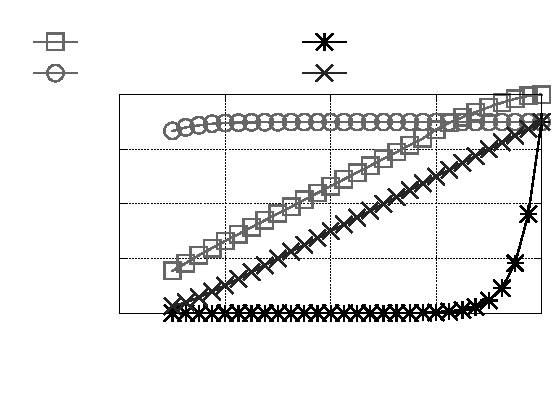
\includegraphics{C-w=2^4}}%
    \gplfronttext
  \end{picture}%
\endgroup
}
\caption{Varying \setSize{\classesUnion} with fixed $\classesSize=2^4$
  and $\setSize{\secretsDomain}=2^{32}$}
\label{fig:model:C}
\end{subfigure}
\hfill
\begin{subfigure}[b]{0.45\columnwidth}
\hspace{-5ex}
\resizebox{\textwidth}{!}{% GNUPLOT: LaTeX picture with Postscript
\begingroup
  \fontfamily{Times-Roman}%
  \selectfont
  \makeatletter
  \providecommand\color[2][]{%
    \GenericError{(gnuplot) \space\space\space\@spaces}{%
      Package color not loaded in conjunction with
      terminal option `colourtext'%
    }{See the gnuplot documentation for explanation.%
    }{Either use 'blacktext' in gnuplot or load the package
      color.sty in LaTeX.}%
    \renewcommand\color[2][]{}%
  }%
  \providecommand\includegraphics[2][]{%
    \GenericError{(gnuplot) \space\space\space\@spaces}{%
      Package graphicx or graphics not loaded%
    }{See the gnuplot documentation for explanation.%
    }{The gnuplot epslatex terminal needs graphicx.sty or graphics.sty.}%
    \renewcommand\includegraphics[2][]{}%
  }%
  \providecommand\rotatebox[2]{#2}%
  \@ifundefined{ifGPcolor}{%
    \newif\ifGPcolor
    \GPcolortrue
  }{}%
  \@ifundefined{ifGPblacktext}{%
    \newif\ifGPblacktext
    \GPblacktexttrue
  }{}%
  % define a \g@addto@macro without @ in the name:
  \let\gplgaddtomacro\g@addto@macro
  % define empty templates for all commands taking text:
  \gdef\gplbacktext{}%
  \gdef\gplfronttext{}%
  \makeatother
  \ifGPblacktext
    % no textcolor at all
    \def\colorrgb#1{}%
    \def\colorgray#1{}%
  \else
    % gray or color?
    \ifGPcolor
      \def\colorrgb#1{\color[rgb]{#1}}%
      \def\colorgray#1{\color[gray]{#1}}%
      \expandafter\def\csname LTw\endcsname{\color{white}}%
      \expandafter\def\csname LTb\endcsname{\color{black}}%
      \expandafter\def\csname LTa\endcsname{\color{black}}%
      \expandafter\def\csname LT0\endcsname{\color[rgb]{1,0,0}}%
      \expandafter\def\csname LT1\endcsname{\color[rgb]{0,1,0}}%
      \expandafter\def\csname LT2\endcsname{\color[rgb]{0,0,1}}%
      \expandafter\def\csname LT3\endcsname{\color[rgb]{1,0,1}}%
      \expandafter\def\csname LT4\endcsname{\color[rgb]{0,1,1}}%
      \expandafter\def\csname LT5\endcsname{\color[rgb]{1,1,0}}%
      \expandafter\def\csname LT6\endcsname{\color[rgb]{0,0,0}}%
      \expandafter\def\csname LT7\endcsname{\color[rgb]{1,0.3,0}}%
      \expandafter\def\csname LT8\endcsname{\color[rgb]{0.5,0.5,0.5}}%
    \else
      % gray
      \def\colorrgb#1{\color{black}}%
      \def\colorgray#1{\color[gray]{#1}}%
      \expandafter\def\csname LTw\endcsname{\color{white}}%
      \expandafter\def\csname LTb\endcsname{\color{black}}%
      \expandafter\def\csname LTa\endcsname{\color{black}}%
      \expandafter\def\csname LT0\endcsname{\color{black}}%
      \expandafter\def\csname LT1\endcsname{\color{black}}%
      \expandafter\def\csname LT2\endcsname{\color{black}}%
      \expandafter\def\csname LT3\endcsname{\color{black}}%
      \expandafter\def\csname LT4\endcsname{\color{black}}%
      \expandafter\def\csname LT5\endcsname{\color{black}}%
      \expandafter\def\csname LT6\endcsname{\color{black}}%
      \expandafter\def\csname LT7\endcsname{\color{black}}%
      \expandafter\def\csname LT8\endcsname{\color{black}}%
    \fi
  \fi
    \setlength{\unitlength}{0.0500bp}%
    \ifx\gptboxheight\undefined%
      \newlength{\gptboxheight}%
      \newlength{\gptboxwidth}%
      \newsavebox{\gptboxtext}%
    \fi%
    \setlength{\fboxrule}{0.5pt}%
    \setlength{\fboxsep}{1pt}%
\begin{picture}(5040.00,3600.00)%
    \gplgaddtomacro\gplbacktext{%
      \csname LTb\endcsname%
      \put(882,750){\makebox(0,0)[r]{\strut{}$0$}}%
      \csname LTb\endcsname%
      \put(882,1275){\makebox(0,0)[r]{\strut{}$8$}}%
      \csname LTb\endcsname%
      \put(882,1800){\makebox(0,0)[r]{\strut{}$16$}}%
      \csname LTb\endcsname%
      \put(882,2324){\makebox(0,0)[r]{\strut{}$24$}}%
      \csname LTb\endcsname%
      \put(882,2849){\makebox(0,0)[r]{\strut{}$32$}}%
      \csname LTb\endcsname%
      \put(990,480){\makebox(0,0){\strut{}$0$}}%
      \csname LTb\endcsname%
      \put(2002,480){\makebox(0,0){\strut{}$8$}}%
      \csname LTb\endcsname%
      \put(3015,480){\makebox(0,0){\strut{}$16$}}%
      \csname LTb\endcsname%
      \put(4027,480){\makebox(0,0){\strut{}$24$}}%
      \csname LTb\endcsname%
      \put(5039,480){\makebox(0,0){\strut{}$32$}}%
    }%
    \gplgaddtomacro\gplfronttext{%
      \csname LTb\endcsname%
      \put(372,1799){\rotatebox{-270}{\makebox(0,0){\strut{}Leakage measures}}}%
      \put(3014,150){\makebox(0,0){\strut{}$\log_2{\frac{\setSize{\secretsDomain}}{\classesSize}}$}}%
      \csname LTb\endcsname%
      \put(763,3355){\makebox(0,0)[l]{\strut{}$\log_2{(\setSize{\secretsDomain}/\secretsSetSizeMin{})}$}}%
      \csname LTb\endcsname%
      \put(763,3055){\makebox(0,0)[l]{\strut{}$\log_2{(\setSize{\secretsDomain}/\secretsSetSizeMax{})}$}}%
      \csname LTb\endcsname%
      \put(3346,3355){\makebox(0,0)[l]{\strut{}\muEntropy}}%
      \csname LTb\endcsname%
      \put(3346,3055){\makebox(0,0)[l]{\strut{}\minEntropy}}%
    }%
    \gplbacktext
    \put(0,0){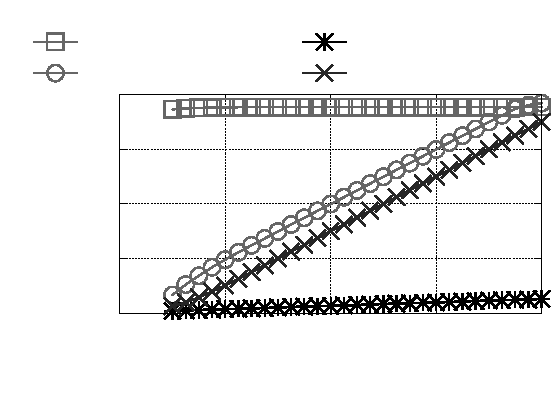
\includegraphics{w-C=2^28}}%
    \gplfronttext
  \end{picture}%
\endgroup
}
\caption{Varying \classesSize with fixed
  $\setSize{\classesUnion}=2^{28}$ and
  $\setSize{\secretsDomain}=2^{32}$}
\label{fig:model:w}
\end{subfigure}
\caption{Relating \secretsSetSizeMin{} and \secretsSetSizeMax{} to
  min-entropy and mutual entropy, for the idealized model of leakage
  explored in \secref{sscf:sec:measurement:secretsSetSize}}
\label{fig:model}
\end{figure}

Roughly speaking, a larger value for \secretsSetSizeMin{} suggests
that information leaks from the procedure for more secret values, and
a larger value for \secretsSetSizeMax{} suggests that more information
leaks from the procedure about secret values.\footnote{While these
rules of thumb are accurate when \Jaccard{\secretsSetSize} has no
valley, they are less reliable when it does.  In such cases, a more
reliable understanding can be obtained by examining the graph of
\Jaccard{\secretsSetSize} directly, or at least by computing a
separate \secretsSetSizeMin{} and \secretsSetSizeMax{} for each
valley-free segment of \Jaccard{\secretsSetSize}.  Here, by ``valley''
we mean values \secretsSetSize, \secretsSetSizeAlt where
$\secretsSetSize < \secretsSetSizeAlt$, $\Jaccard{\secretsSetSize} >
\Jaccard{\secretsSetSize+1}$, $\Jaccard{\secretsSetSizeAlt} <
\Jaccard{\secretsSetSizeAlt+1}$, and $\Jaccard{\secretsSetSizeAltAlt}
= \Jaccard{\secretsSetSizeAltAlt+1}$ for each $\secretsSetSizeAltAlt
\in [\secretsSetSize+1, \secretsSetSizeAlt-1]$.  We have not
encountered \Jaccard{\secretsSetSize} curves with valleys in practice,
and so do not discuss them further here.}  To relate these measures to
another used previously in the \gls{QIF} literature, namely min-entropy
(e.g.,~\cite{geoffrey2011,doi:10.1137/060651380}), in
\figref{fig:model} we show \secretsSetSizeMin{} and
\secretsSetSizeMax{} in comparison to the min-entropy of
$\SecFn{}(\secretVar)$, for our idealized setting above.
\figref{fig:model:C} shows that \secretsSetSizeMin{} reflects the
growth of \setSize{\classesUnion} just as min-entropy can, and
similarly, \figref{fig:model:w} shows that \secretsSetSizeMax{}
reflects changes in \classesSize like min-entropy can.  However,
min-entropy does not distinguish between these types of leakage.
Mutual entropy
(e.g.,~\cite{Clark:2005:QIF,Kopf:2007:IMA:1315245.1315282,Malacaria:2007:AST})
also reflects increasing leakage as \setSize{\classesUnion} grows in
\figref{fig:model:C} and as \classesSize shrinks in
\figref{fig:model:w}, though its sensitivity to these effects is
limited, particularly that of increasing \setSize{\classesUnion},
until \setSize{\classesUnion} becomes quite large
(\figref{fig:model:C}).

\subsection{Procedures with other inputs}
\label{sscf:sec:measurement:random}

The measures \Jaccard{\secretsSetSize}, \secretsSetSizeMin{}, and
\secretsSetSizeMax{} are appropriate when \proc is deterministic and
leverages no inputs in \AIIFn{}.  When either of these restrictions
are lifted, our approach described so far can be unreliable.  
We
illustrate this in \secref{sscf:sec:measurement:random:limits} and then
provide an alternative measure in
\secref{sscf:sec:measurement:random:measure} that is more robust.

\subsubsection{Limitations of \Jaccard{\secretsSetSize}}
\label{sscf:sec:measurement:random:limits}

\begin{figure}
  \begin{subfigure}[b]{0.32\linewidth}
  \centering
  \footnotesize{
\begin{tabbing}
      ** \= ** \= \kill
      \proc(\ACIFn{}, \AIIFn{}, \SecFn{}) \\
      \>  if ($\SecFn{}(\secretVar) = \ACIFn{}(\textrm{`test'})$) \\
      \> \> $\AOOFn{}(\textrm{`result'}) \gets \mathit{rand}()\bmod \modulus$ \\
      \>  else \\
      \> \>  $\AOOFn{}(\textrm{`result'}) \gets \modulus + (\mathit{rand}() \bmod 16)$ \\
      \> return \AOOFn{} 
    \end{tabbing}
    \vspace{3ex}
    }
    \caption{Procedure}
    \label{fig:inflating:code}
  \end{subfigure}
\hspace{-2ex}
  \begin{subfigure}[b]{0.32\linewidth}
  \centering
  \resizebox{0.96\linewidth}{!}{\large% GNUPLOT: LaTeX picture with Postscript
\begingroup
  \fontfamily{Times-Roman}%
  \selectfont
  \makeatletter
  \providecommand\color[2][]{%
    \GenericError{(gnuplot) \space\space\space\@spaces}{%
      Package color not loaded in conjunction with
      terminal option `colourtext'%
    }{See the gnuplot documentation for explanation.%
    }{Either use 'blacktext' in gnuplot or load the package
      color.sty in LaTeX.}%
    \renewcommand\color[2][]{}%
  }%
  \providecommand\includegraphics[2][]{%
    \GenericError{(gnuplot) \space\space\space\@spaces}{%
      Package graphicx or graphics not loaded%
    }{See the gnuplot documentation for explanation.%
    }{The gnuplot epslatex terminal needs graphicx.sty or graphics.sty.}%
    \renewcommand\includegraphics[2][]{}%
  }%
  \providecommand\rotatebox[2]{#2}%
  \@ifundefined{ifGPcolor}{%
    \newif\ifGPcolor
    \GPcolortrue
  }{}%
  \@ifundefined{ifGPblacktext}{%
    \newif\ifGPblacktext
    \GPblacktexttrue
  }{}%
  % define a \g@addto@macro without @ in the name:
  \let\gplgaddtomacro\g@addto@macro
  % define empty templates for all commands taking text:
  \gdef\gplbacktext{}%
  \gdef\gplfronttext{}%
  \makeatother
  \ifGPblacktext
    % no textcolor at all
    \def\colorrgb#1{}%
    \def\colorgray#1{}%
  \else
    % gray or color?
    \ifGPcolor
      \def\colorrgb#1{\color[rgb]{#1}}%
      \def\colorgray#1{\color[gray]{#1}}%
      \expandafter\def\csname LTw\endcsname{\color{white}}%
      \expandafter\def\csname LTb\endcsname{\color{black}}%
      \expandafter\def\csname LTa\endcsname{\color{black}}%
      \expandafter\def\csname LT0\endcsname{\color[rgb]{1,0,0}}%
      \expandafter\def\csname LT1\endcsname{\color[rgb]{0,1,0}}%
      \expandafter\def\csname LT2\endcsname{\color[rgb]{0,0,1}}%
      \expandafter\def\csname LT3\endcsname{\color[rgb]{1,0,1}}%
      \expandafter\def\csname LT4\endcsname{\color[rgb]{0,1,1}}%
      \expandafter\def\csname LT5\endcsname{\color[rgb]{1,1,0}}%
      \expandafter\def\csname LT6\endcsname{\color[rgb]{0,0,0}}%
      \expandafter\def\csname LT7\endcsname{\color[rgb]{1,0.3,0}}%
      \expandafter\def\csname LT8\endcsname{\color[rgb]{0.5,0.5,0.5}}%
    \else
      % gray
      \def\colorrgb#1{\color{black}}%
      \def\colorgray#1{\color[gray]{#1}}%
      \expandafter\def\csname LTw\endcsname{\color{white}}%
      \expandafter\def\csname LTb\endcsname{\color{black}}%
      \expandafter\def\csname LTa\endcsname{\color{black}}%
      \expandafter\def\csname LT0\endcsname{\color{black}}%
      \expandafter\def\csname LT1\endcsname{\color{black}}%
      \expandafter\def\csname LT2\endcsname{\color{black}}%
      \expandafter\def\csname LT3\endcsname{\color{black}}%
      \expandafter\def\csname LT4\endcsname{\color{black}}%
      \expandafter\def\csname LT5\endcsname{\color{black}}%
      \expandafter\def\csname LT6\endcsname{\color{black}}%
      \expandafter\def\csname LT7\endcsname{\color{black}}%
      \expandafter\def\csname LT8\endcsname{\color{black}}%
    \fi
  \fi
    \setlength{\unitlength}{0.0500bp}%
    \ifx\gptboxheight\undefined%
      \newlength{\gptboxheight}%
      \newlength{\gptboxwidth}%
      \newsavebox{\gptboxtext}%
    \fi%
    \setlength{\fboxrule}{0.5pt}%
    \setlength{\fboxsep}{1pt}%
\begin{picture}(4896.00,2736.00)%
    \gplgaddtomacro\gplbacktext{%
      \csname LTb\endcsname%
      \put(691,600){\makebox(0,0)[r]{\strut{}$0$}}%
      \csname LTb\endcsname%
      \put(691,1031){\makebox(0,0)[r]{\strut{}$0.2$}}%
      \csname LTb\endcsname%
      \put(691,1462){\makebox(0,0)[r]{\strut{}$0.4$}}%
      \csname LTb\endcsname%
      \put(691,1892){\makebox(0,0)[r]{\strut{}$0.6$}}%
      \csname LTb\endcsname%
      \put(691,2323){\makebox(0,0)[r]{\strut{}$0.8$}}%
      \csname LTb\endcsname%
      \put(792,312){\makebox(0,0){\strut{}$0$}}%
      \csname LTb\endcsname%
      \put(1303,312){\makebox(0,0){\strut{}$4$}}%
      \csname LTb\endcsname%
      \put(1814,312){\makebox(0,0){\strut{}$8$}}%
      \csname LTb\endcsname%
      \put(2325,312){\makebox(0,0){\strut{}$12$}}%
      \csname LTb\endcsname%
      \put(2836,312){\makebox(0,0){\strut{}$16$}}%
      \csname LTb\endcsname%
      \put(3347,312){\makebox(0,0){\strut{}$20$}}%
      \csname LTb\endcsname%
      \put(3858,312){\makebox(0,0){\strut{}$24$}}%
      \csname LTb\endcsname%
      \put(4369,312){\makebox(0,0){\strut{}$28$}}%
      \csname LTb\endcsname%
      \put(4880,312){\makebox(0,0){\strut{}$32$}}%
    }%
    \gplgaddtomacro\gplfronttext{%
      \csname LTb\endcsname%
      \put(240,1655){\rotatebox{-270}{\makebox(0,0){\strut{}\Jaccard{\secretsSetSize}}}}%
      \put(2836,96){\makebox(0,0){\strut{}$\log_2{\secretsSetSize}$}}%
      \csname LTb\endcsname%
      \put(1575,2528){\makebox(0,0)[l]{\strut{}\modulus=$1$}}%
      \csname LTb\endcsname%
      \put(1575,2288){\makebox(0,0)[l]{\strut{}\modulus=$4$}}%
      \csname LTb\endcsname%
      \put(1575,2048){\makebox(0,0)[l]{\strut{}\modulus=$8$}}%
      \csname LTb\endcsname%
      \put(3222,2528){\makebox(0,0)[l]{\strut{}\modulus=$16$}}%
      \csname LTb\endcsname%
      \put(3222,2288){\makebox(0,0)[l]{\strut{}\modulus=$64$}}%
      \csname LTb\endcsname%
      \put(3222,2048){\makebox(0,0)[l]{\strut{}\modulus=$2^{10}$}}%
    }%
    \gplbacktext
    \put(0,0){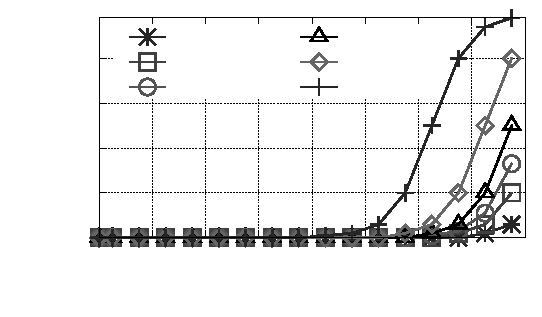
\includegraphics{inflate}}%
    \gplfronttext
  \end{picture}%
\endgroup
}
    \caption{\Jaccard{\secretsSetSize} for various \secretsSetSize and \modulus}
    \label{fig:inflating:Jaccard}
  \end{subfigure}%
\hspace{-3ex}
  \begin{subfigure}[b]{0.32\linewidth}
  \centering
  \resizebox{0.96\linewidth}{!}{\large% GNUPLOT: LaTeX picture with Postscript
\begingroup
  \fontfamily{Times-Roman}%
  \selectfont
  \makeatletter
  \providecommand\color[2][]{%
    \GenericError{(gnuplot) \space\space\space\@spaces}{%
      Package color not loaded in conjunction with
      terminal option `colourtext'%
    }{See the gnuplot documentation for explanation.%
    }{Either use 'blacktext' in gnuplot or load the package
      color.sty in LaTeX.}%
    \renewcommand\color[2][]{}%
  }%
  \providecommand\includegraphics[2][]{%
    \GenericError{(gnuplot) \space\space\space\@spaces}{%
      Package graphicx or graphics not loaded%
    }{See the gnuplot documentation for explanation.%
    }{The gnuplot epslatex terminal needs graphicx.sty or graphics.sty.}%
    \renewcommand\includegraphics[2][]{}%
  }%
  \providecommand\rotatebox[2]{#2}%
  \@ifundefined{ifGPcolor}{%
    \newif\ifGPcolor
    \GPcolortrue
  }{}%
  \@ifundefined{ifGPblacktext}{%
    \newif\ifGPblacktext
    \GPblacktexttrue
  }{}%
  % define a \g@addto@macro without @ in the name:
  \let\gplgaddtomacro\g@addto@macro
  % define empty templates for all commands taking text:
  \gdef\gplbacktext{}%
  \gdef\gplfronttext{}%
  \makeatother
  \ifGPblacktext
    % no textcolor at all
    \def\colorrgb#1{}%
    \def\colorgray#1{}%
  \else
    % gray or color?
    \ifGPcolor
      \def\colorrgb#1{\color[rgb]{#1}}%
      \def\colorgray#1{\color[gray]{#1}}%
      \expandafter\def\csname LTw\endcsname{\color{white}}%
      \expandafter\def\csname LTb\endcsname{\color{black}}%
      \expandafter\def\csname LTa\endcsname{\color{black}}%
      \expandafter\def\csname LT0\endcsname{\color[rgb]{1,0,0}}%
      \expandafter\def\csname LT1\endcsname{\color[rgb]{0,1,0}}%
      \expandafter\def\csname LT2\endcsname{\color[rgb]{0,0,1}}%
      \expandafter\def\csname LT3\endcsname{\color[rgb]{1,0,1}}%
      \expandafter\def\csname LT4\endcsname{\color[rgb]{0,1,1}}%
      \expandafter\def\csname LT5\endcsname{\color[rgb]{1,1,0}}%
      \expandafter\def\csname LT6\endcsname{\color[rgb]{0,0,0}}%
      \expandafter\def\csname LT7\endcsname{\color[rgb]{1,0.3,0}}%
      \expandafter\def\csname LT8\endcsname{\color[rgb]{0.5,0.5,0.5}}%
    \else
      % gray
      \def\colorrgb#1{\color{black}}%
      \def\colorgray#1{\color[gray]{#1}}%
      \expandafter\def\csname LTw\endcsname{\color{white}}%
      \expandafter\def\csname LTb\endcsname{\color{black}}%
      \expandafter\def\csname LTa\endcsname{\color{black}}%
      \expandafter\def\csname LT0\endcsname{\color{black}}%
      \expandafter\def\csname LT1\endcsname{\color{black}}%
      \expandafter\def\csname LT2\endcsname{\color{black}}%
      \expandafter\def\csname LT3\endcsname{\color{black}}%
      \expandafter\def\csname LT4\endcsname{\color{black}}%
      \expandafter\def\csname LT5\endcsname{\color{black}}%
      \expandafter\def\csname LT6\endcsname{\color{black}}%
      \expandafter\def\csname LT7\endcsname{\color{black}}%
      \expandafter\def\csname LT8\endcsname{\color{black}}%
    \fi
  \fi
    \setlength{\unitlength}{0.0500bp}%
    \ifx\gptboxheight\undefined%
      \newlength{\gptboxheight}%
      \newlength{\gptboxwidth}%
      \newsavebox{\gptboxtext}%
    \fi%
    \setlength{\fboxrule}{0.5pt}%
    \setlength{\fboxsep}{1pt}%
\begin{picture}(4896.00,2736.00)%
    \gplgaddtomacro\gplbacktext{%
      \csname LTb\endcsname%
      \put(691,600){\makebox(0,0)[r]{\strut{}$0$}}%
      \csname LTb\endcsname%
      \put(691,1436){\makebox(0,0)[r]{\strut{}$0.2$}}%
      \csname LTb\endcsname%
      \put(691,2272){\makebox(0,0)[r]{\strut{}$0.4$}}%
      \csname LTb\endcsname%
      \put(792,312){\makebox(0,0){\strut{}$0$}}%
      \csname LTb\endcsname%
      \put(1303,312){\makebox(0,0){\strut{}$4$}}%
      \csname LTb\endcsname%
      \put(1814,312){\makebox(0,0){\strut{}$8$}}%
      \csname LTb\endcsname%
      \put(2325,312){\makebox(0,0){\strut{}$12$}}%
      \csname LTb\endcsname%
      \put(2836,312){\makebox(0,0){\strut{}$16$}}%
      \csname LTb\endcsname%
      \put(3347,312){\makebox(0,0){\strut{}$20$}}%
      \csname LTb\endcsname%
      \put(3858,312){\makebox(0,0){\strut{}$24$}}%
      \csname LTb\endcsname%
      \put(4369,312){\makebox(0,0){\strut{}$28$}}%
      \csname LTb\endcsname%
      \put(4880,312){\makebox(0,0){\strut{}$32$}}%
    }%
    \gplgaddtomacro\gplfronttext{%
      \csname LTb\endcsname%
      \put(240,1655){\rotatebox{-270}{\makebox(0,0){\strut{}\JaccardRand{\secretsSetSize}}}}%
      \put(2836,96){\makebox(0,0){\strut{}$\log_2{\secretsSetSize}$}}%
      \csname LTb\endcsname%
      \put(1575,2528){\makebox(0,0)[l]{\strut{}\modulus=$1$}}%
      \csname LTb\endcsname%
      \put(1575,2288){\makebox(0,0)[l]{\strut{}\modulus=$4$}}%
      \csname LTb\endcsname%
      \put(1575,2048){\makebox(0,0)[l]{\strut{}\modulus=$8$}}%
      \csname LTb\endcsname%
      \put(3222,2528){\makebox(0,0)[l]{\strut{}\modulus=$16$}}%
      \csname LTb\endcsname%
      \put(3222,2288){\makebox(0,0)[l]{\strut{}\modulus=$64$}}%
      \csname LTb\endcsname%
      \put(3222,2048){\makebox(0,0)[l]{\strut{}\modulus=$2^{10}$}}%
    }%
    \gplbacktext
    \put(0,0){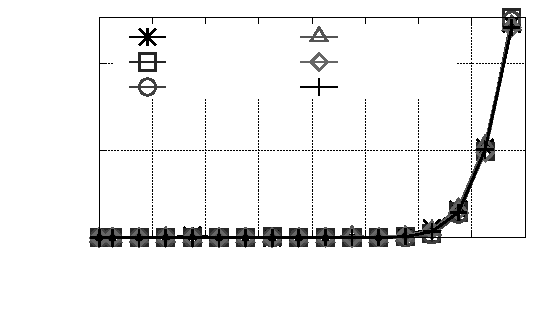
\includegraphics{inflate-fix}}%
    \gplfronttext
  \end{picture}%
\endgroup
}
    \caption{\JaccardRand{\secretsSetSize} for various \secretsSetSize and \modulus}
    \label{fig:inflating:JaccardRand}
  \end{subfigure}
  \caption{An example showing limitations of \Jaccard{} on
    procedures with randomness and improvements offered by
    \JaccardRand{} (see \secref{sscf:sec:measurement:random})}
  \label{fig:inflating}
\end{figure}

First consider a randomized password checker that receives a secret
password $\SecFn{}(\secretVar)$ and a candidate password
$\ACIFn{}(\textrm{`test'})$ and, for some constant $\modulus > 0$,
outputs a random value in $[0, \modulus-1]$ if the candidate password
is equal to the secret password and random value in $[\modulus,
  \modulus+16]$ otherwise.  Intuitively, the leakage of this procedure
should be the same as a deterministic password checker and independent
of the value of \modulus.  However, as shown in
\figref{fig:inflating}, the use of randomness here results in an
unintuitive result, since \Jaccard{\secretsSetSize}
(\figref{fig:inflating:Jaccard}) is sensitive to the value of
\modulus.  As such, while our detector does accurately detect leakage
in this case, it provides less help in comparing the leakage of two
randomized implementations.

Another problem may arise when other inputs are allowed in \AIIFn{}.
Consider the example
\begin{tabbing}
  **** \= ** \= \kill
  \> \proc(\ACIFn{}, \AIIFn{}, \SecFn{}) \\
  \> \> $\AOOFn{}(\textrm{`result'}) \gets$
     \= $((\SecFn{}(\secretVar)  > \ACIFn{}(\textrm{`test'}))~?~1~:~0)$
   $\oplus~((\AIIFn{}(\textrm{`other'}) \le 0)~?~1~:~0)$ \\
  \> \> return \AOOFn{}
\end{tabbing}
Here, the expression ``\textit{cond}~?~1~:~0'' evaluates to $1$ if
\textit{cond} is true and $0$ otherwise, and ``$\oplus$'' represents
XOR.  This procedure indicates that $\SecFn{}(\secretVar) >
\ACIFn{}(\textrm{`test'})$ by returning $0$ if
$\AIIFn{}(\textrm{`other'}) \le 0$ or by returning $1$ if
$\AIIFn{}(\textrm{`other'}) > 0$.  Because our technique allows for
any value of $\AIIFn{}(\textrm{`other'})$ consistent with
\postcondition{\proc}{} when estimating
\setSize{\possibleDoubles{\secretsSet{}}}, it will compute
$\Jaccard{\secretsSetSize} = 0$ for any \secretsSetSize, suggesting no
leakage.  However, the only condition under which \proc in fact leaks
no information is if $\AIIFn{}(\textrm{`other'})$ is non-positive or
positive with equal probability from the adversary's perspective.

\subsubsection{An alternative measure}
\label{sscf:sec:measurement:random:measure}

To overcome the limitations of \Jaccard{\secretsSetSize} as
illustrated above, in this section we propose a leakage measure that
is more robust for procedures that employ randomness or inputs in
\AIIFn{}.  For convenience, here we treat all values generated at
random within the procedure instead as inputs represented in \AIIFn{};
e.g., the first invocation of \texttt{rand()} within the procedure is
replaced with a reference to, say, $\AIIFn{}(\textrm{`rand[1]'})$, the
second with $\AIIFn{}(\textrm{`rand[2]'})$, and so forth.
Intuitively, our measure employs an alternative definition for
\possibleDoubles{\secretsSet{}} that also includes these additional
inputs.  Specifically, consider the set \possibleTriplesIntersect{\secretsSet{}}{\secretsSetAlt{}}
\if0
\[
\possibleTriplesIntersect{\secretsSet{}}{\secretsSetAlt{}}
= \left\{\langle\ACIFn{}, \AOOFn{}, \AIIFn{}\rangle
~\left|~ \langle\ACIFn{}, \AOOFn{}, \AIIFn{}\rangle \in \possibleTriples{\secretsSet{}} \wedge \langle\ACIFn{}, \AOOFn{} \rangle \in \possibleDoubles{\secretsSet{}} \cap \possibleDoubles{\secretsSetAlt{}}\right.\right\}
\]
\fi

\begin{align}
\possibleTriplesUnion{\secretsSet{}}{\secretsSetAlt{}}& =
\possibleTriples{\secretsSet{}} \cup
\possibleTriples{\secretsSetAlt{}}\nonumber\\
\possibleTriplesIntersect{\secretsSet{}}{\secretsSetAlt{}}
&= \left\{\langle\ACIFn{}, \AOOFn{}, \AIIFn{}\rangle \left| 
  \langle\ACIFn{}, \AOOFn{}, \AIIFn{}\rangle\!\in\! \possibleTriplesUnion{\secretsSet{}}{\secretsSetAlt{}}
  \wedge\langle\ACIFn{}, \AOOFn{} \rangle \!\in\! \possibleDoubles{\secretsSet{}} \!\cap\! \possibleDoubles{\secretsSetAlt{}}
\right.\!\right\}
\nonumber
%\label{eq:possibleTriplesIntersect}
\end{align}

of $\langle \ACIFn{}, \AOOFn{}, \AIIFn{} \rangle$ triples such that
not only is $\langle \ACIFn{}, \AOOFn{} \rangle \in
\possibleDoubles{\secretsSet{}} \cap
\possibleDoubles{\secretsSetAlt{}}$ (c.f., the definition of
$\Jaccard{}(\secretsSet{}, \secretsSetAlt{})$ in
\eqnref{eq:oneJaccard}), but also the triple is consistent with some
$\secretVal \in \secretsSet{}$ (i.e., $\langle\ACIFn{}, \AOOFn{},
\AIIFn{}\rangle \in \possibleTriples{\secretsSet{}}$ where
$\possibleTriples{\secretsSet{}} = \bigcup_{\secretVal
  \in \secretsSet{}} \possibleTriples{\secretVal}$).  By counting
such $\langle \ACIFn{}, \AOOFn{}, \AIIFn{} \rangle$ triples, the
various random values (represented in \AIIFn{}) become exposed in
\possibleTriplesIntersect{\secretsSet{}}{\secretsSetAlt{}} and the
number of these values for a given $\langle \ACIFn{}, \AOOFn{}
\rangle$ pair act as the ``weight'' of that pair. When
$\langle\ACIFn{}{}, \AOOFn{}, \AIIFn{}\rangle$ is from the following
difference set, an attacker can determine whether the secret is from
\secretsSet{} or \secretsSetAlt{}.
\begin{align}
 \possibleTriplesDiff{\secretsSet{}}{\secretsSetAlt{}} = \possibleTriplesUnion{\secretsSet{}}{\secretsSetAlt{}}\setminus\possibleTriplesIntersect{\secretsSet{}}{\secretsSetAlt{}}
\end{align}

We adjust the measure to
\begin{align}
  \JaccardRand{}(\secretsSet{}, \secretsSetAlt{})
  &= \frac{\setSize{\possibleTriplesDiff{\secretsSet{}}{\secretsSetAlt{}}}}{\setSize{\possibleTriplesUnion{\secretsSet{}}{\secretsSetAlt{}}}}
  = 1 - \frac{\setSize{\possibleTriplesIntersect{\secretsSet{}}{\secretsSetAlt{}}}}{\setSize{\possibleTriplesUnion{\secretsSet{}}{\secretsSetAlt{}}}} 
\label{eqn:jaccard}\\
\JaccardRand{\secretsSetSize}
&= \avg_{\scriptsize \begin{array}{r@{\hspace{0.25em}}r} \scriptsize \secretsSet{},\secretsSetAlt{}: & \setSize{\secretsSet{}} = \setSize{\secretsSetAlt{}} = \secretsSetSize \\ & \wedge~\hfill \secretsSet{} \cap \secretsSetAlt{} = \emptyset\end{array}}
\JaccardRand{}(\secretsSet{}, \secretsSetAlt{})
\label{dfn:jaccardRand}
\end{align}

Note that if $\AIIKeys=\emptyset$, then
$\JaccardRand{\secretsSetSize}=\Jaccard{\secretsSetSize}$ since in
this case, $\langle \ACIFn{}, \AOOFn{} \rangle \in
\possibleDoubles{\secretsSet{}}$ if and only if $\langle \ACIFn{},
\AOOFn{}, \emptyset \rangle \in \possibleTriples{\secretsSet{}}$.

The benefit of \JaccardRand{\secretsSetSize} is that it is far less
susceptible to the variability that was demonstrated in
\secref{sscf:sec:measurement:random:limits}.  For example,
\figref{fig:inflating:JaccardRand} shows that this measure is stable,
independent of \modulus.  As we will see in subsequent sections,
however, it is also considerably costlier to estimate.

When we use \JaccardRand{\secretsSetSize} in place of
\Jaccard{\secretsSetSize}, we will annotate measures derived from it
using similar notation.  For example, \secretsSetSizeMinRand{} denotes
\secretsSetSizeMin{} computed using \JaccardRand{\secretsSetSize} in
place of \Jaccard{\secretsSetSize}, and similarly for
\secretsSetSizeMaxRand{}.


\section{Implementation}
\label{sscf:sec:impl}
\begin{figure*}
{
\centering
\resizebox{1.0\textwidth}{!}{\large% Graphic for TeX using PGF
% Title: /Users/ziqiaozhou/sscf/sp2/fig/workflow-loop.dia
% Creator: Dia v0.97.2
% CreationDate: Thu Jan 25 11:12:43 2018
% For: ziqiaozhou
% \usepackage{tikz}
% The following commands are not supported in PSTricks at present
% We define them conditionally, so when they are implemented,
% this pgf file will use them.
\ifx\du\undefined
  \newlength{\du}
\fi
\setlength{\du}{15\unitlength}
\begin{tikzpicture}
\pgftransformxscale{1.000000}
\pgftransformyscale{-1.000000}
\definecolor{dialinecolor}{rgb}{0.000000, 0.000000, 0.000000}
\pgfsetstrokecolor{dialinecolor}
\definecolor{dialinecolor}{rgb}{1.000000, 1.000000, 1.000000}
\pgfsetfillcolor{dialinecolor}
\definecolor{dialinecolor}{rgb}{1.000000, 1.000000, 1.000000}
\pgfsetfillcolor{dialinecolor}
\fill (32.472400\du,2.949270\du)--(32.472400\du,8.313852\du)--(46.411342\du,8.313852\du)--(46.411342\du,2.949270\du)--cycle;
\pgfsetlinewidth{0.100000\du}
\pgfsetdash{}{0pt}
\pgfsetdash{}{0pt}
\pgfsetmiterjoin
\definecolor{dialinecolor}{rgb}{0.000000, 0.000000, 0.000000}
\pgfsetstrokecolor{dialinecolor}
\draw (32.472400\du,2.949270\du)--(32.472400\du,8.313852\du)--(46.411342\du,8.313852\du)--(46.411342\du,2.949270\du)--cycle;
% setfont left to latex
\definecolor{dialinecolor}{rgb}{0.000000, 0.000000, 0.000000}
\pgfsetstrokecolor{dialinecolor}
\node at (39.441871\du,5.874747\du){};
\definecolor{dialinecolor}{rgb}{1.000000, 1.000000, 1.000000}
\pgfsetfillcolor{dialinecolor}
\fill (31.018700\du,3.200720\du)--(31.018700\du,8.603813\du)--(44.478732\du,8.603813\du)--(44.478732\du,3.200720\du)--cycle;
\pgfsetlinewidth{0.100000\du}
\pgfsetdash{{1.000000\du}{1.000000\du}}{0\du}
\pgfsetdash{{0.400000\du}{0.400000\du}}{0\du}
\pgfsetmiterjoin
\definecolor{dialinecolor}{rgb}{0.000000, 0.000000, 0.000000}
\pgfsetstrokecolor{dialinecolor}
\draw (31.018700\du,3.200720\du)--(31.018700\du,8.603813\du)--(44.478732\du,8.603813\du)--(44.478732\du,3.200720\du)--cycle;
% setfont left to latex
\definecolor{dialinecolor}{rgb}{0.000000, 0.000000, 0.000000}
\pgfsetstrokecolor{dialinecolor}
\node at (37.748716\du,6.145452\du){};
\definecolor{dialinecolor}{rgb}{1.000000, 1.000000, 1.000000}
\pgfsetfillcolor{dialinecolor}
\fill (29.597600\du,3.497390\du)--(29.597600\du,8.893773\du)--(43.250000\du,8.893773\du)--(43.250000\du,3.497390\du)--cycle;
\pgfsetlinewidth{0.100000\du}
\pgfsetdash{}{0pt}
\pgfsetdash{}{0pt}
\pgfsetmiterjoin
\definecolor{dialinecolor}{rgb}{0.000000, 0.000000, 0.000000}
\pgfsetstrokecolor{dialinecolor}
\draw (29.597600\du,3.497390\du)--(29.597600\du,8.893773\du)--(43.250000\du,8.893773\du)--(43.250000\du,3.497390\du)--cycle;
% setfont left to latex
\definecolor{dialinecolor}{rgb}{0.000000, 0.000000, 0.000000}
\pgfsetstrokecolor{dialinecolor}
\node at (36.423800\du,6.438768\du){};
\definecolor{dialinecolor}{rgb}{1.000000, 1.000000, 1.000000}
\pgfsetfillcolor{dialinecolor}
\fill (9.382400\du,5.382180\du)--(9.382400\du,7.663295\du)--(16.617400\du,7.663295\du)--(16.617400\du,5.382180\du)--cycle;
\pgfsetlinewidth{0.100000\du}
\pgfsetdash{}{0pt}
\pgfsetdash{}{0pt}
\pgfsetmiterjoin
\definecolor{dialinecolor}{rgb}{0.000000, 0.000000, 0.000000}
\pgfsetstrokecolor{dialinecolor}
\draw (9.382400\du,5.382180\du)--(9.382400\du,7.663295\du)--(16.617400\du,7.663295\du)--(16.617400\du,5.382180\du)--cycle;
% setfont left to latex
\definecolor{dialinecolor}{rgb}{0.000000, 0.000000, 0.000000}
\pgfsetstrokecolor{dialinecolor}
\node at (12.999900\du,6.765924\du){};
\definecolor{dialinecolor}{rgb}{1.000000, 1.000000, 1.000000}
\pgfsetfillcolor{dialinecolor}
\fill (4.767976\du,5.823180\du)--(7.901175\du,5.823180\du)--(7.353899\du,7.326808\du)--(4.220700\du,7.326808\du)--cycle;
\pgfsetlinewidth{0.100000\du}
\pgfsetdash{}{0pt}
\pgfsetdash{}{0pt}
\pgfsetmiterjoin
\definecolor{dialinecolor}{rgb}{0.000000, 0.000000, 0.000000}
\pgfsetstrokecolor{dialinecolor}
\draw (4.767976\du,5.823180\du)--(7.901175\du,5.823180\du)--(7.353899\du,7.326808\du)--(4.220700\du,7.326808\du)--cycle;
% setfont left to latex
\definecolor{dialinecolor}{rgb}{0.000000, 0.000000, 0.000000}
\pgfsetstrokecolor{dialinecolor}
\node at (6.060937\du,6.818180\du){};
\pgfsetlinewidth{0.200000\du}
\pgfsetdash{}{0pt}
\pgfsetdash{}{0pt}
\pgfsetbuttcap
{
\definecolor{dialinecolor}{rgb}{0.000000, 0.000000, 0.000000}
\pgfsetfillcolor{dialinecolor}
% was here!!!
\pgfsetarrowsend{latex}
\definecolor{dialinecolor}{rgb}{0.000000, 0.000000, 0.000000}
\pgfsetstrokecolor{dialinecolor}
\draw (7.627537\du,6.574994\du)--(9.382400\du,6.522740\du);
}
\pgfsetlinewidth{0.200000\du}
\pgfsetdash{}{0pt}
\pgfsetdash{}{0pt}
\pgfsetbuttcap
{
\definecolor{dialinecolor}{rgb}{0.000000, 0.000000, 0.000000}
\pgfsetfillcolor{dialinecolor}
% was here!!!
\pgfsetarrowsend{stealth}
\definecolor{dialinecolor}{rgb}{0.000000, 0.000000, 0.000000}
\pgfsetstrokecolor{dialinecolor}
\draw (16.617400\du,6.522740\du)--(19.338100\du,6.535535\du);
}
\pgfsetlinewidth{0.100000\du}
\pgfsetdash{}{0pt}
\pgfsetdash{}{0pt}
\pgfsetmiterjoin
\definecolor{dialinecolor}{rgb}{1.000000, 1.000000, 1.000000}
\pgfsetfillcolor{dialinecolor}
\fill (48.356300\du,4.232730\du)--(48.356300\du,7.361161\du)--(54.170223\du,7.361161\du)--(54.170223\du,4.232730\du)--cycle;
\definecolor{dialinecolor}{rgb}{0.000000, 0.000000, 0.000000}
\pgfsetstrokecolor{dialinecolor}
\draw (48.356300\du,4.232730\du)--(48.356300\du,7.361161\du)--(54.170223\du,7.361161\du)--(54.170223\du,4.232730\du)--cycle;
% setfont left to latex
\definecolor{dialinecolor}{rgb}{0.000000, 0.000000, 0.000000}
\pgfsetstrokecolor{dialinecolor}
\node[anchor=west] at (48.981400\du,4.835722\du){Compute \Jaccard{\secretsSetSize},};
% setfont left to latex
\definecolor{dialinecolor}{rgb}{0.000000, 0.000000, 0.000000}
\pgfsetstrokecolor{dialinecolor}
\node[anchor=west] at (48.981400\du,5.639350\du){\secretsSetSizeMin{} and \secretsSetSizeMax{}};
% setfont left to latex
\definecolor{dialinecolor}{rgb}{0.000000, 0.000000, 0.000000}
\pgfsetstrokecolor{dialinecolor}
\node[anchor=west] at (48.981400\du,6.442978\du){(\secref{sscf:sec:measurement:secretsSetSize})};
\pgfsetlinewidth{0.200000\du}
\pgfsetdash{}{0pt}
\pgfsetdash{}{0pt}
\pgfsetbuttcap
{
\definecolor{dialinecolor}{rgb}{0.000000, 0.000000, 0.000000}
\pgfsetfillcolor{dialinecolor}
% was here!!!
\pgfsetarrowsend{stealth}
\definecolor{dialinecolor}{rgb}{0.000000, 0.000000, 0.000000}
\pgfsetstrokecolor{dialinecolor}
\draw (46.461222\du,5.761787\du)--(48.356300\du,5.796946\du);
}
% setfont left to latex
\definecolor{dialinecolor}{rgb}{0.000000, 0.000000, 0.000000}
\pgfsetstrokecolor{dialinecolor}
\node[anchor=west] at (16.510700\du,5.187180\du){\postcondition{\proc}{}};
% setfont left to latex
\definecolor{dialinecolor}{rgb}{0.000000, 0.000000, 0.000000}
\pgfsetstrokecolor{dialinecolor}
\node at (12.990400\du,6.079380\du){Symbolic Execution};
% setfont left to latex
\definecolor{dialinecolor}{rgb}{0.000000, 0.000000, 0.000000}
\pgfsetstrokecolor{dialinecolor}
\node at (12.990400\du,6.879380\du){(\secref{sscf:sec:symbolic})};
\pgfsetlinewidth{0.200000\du}
\pgfsetdash{}{0pt}
\pgfsetdash{}{0pt}
\pgfsetbuttcap
{
\definecolor{dialinecolor}{rgb}{0.000000, 0.000000, 0.000000}
\pgfsetfillcolor{dialinecolor}
% was here!!!
\definecolor{dialinecolor}{rgb}{0.000000, 0.000000, 0.000000}
\pgfsetstrokecolor{dialinecolor}
\draw (5.003150\du,8.264880\du)--(5.004000\du,7.326808\du);
}
% setfont left to latex
\definecolor{dialinecolor}{rgb}{0.000000, 0.000000, 0.000000}
\pgfsetstrokecolor{dialinecolor}
\node at (4.965880\du,8.991080\du){\ACIFn{}};
% setfont left to latex
\definecolor{dialinecolor}{rgb}{0.000000, 0.000000, 0.000000}
\pgfsetstrokecolor{dialinecolor}
\node[anchor=west] at (5.059390\du,6.658680\du){\proc};
% setfont left to latex
\definecolor{dialinecolor}{rgb}{0.000000, 0.000000, 0.000000}
\pgfsetstrokecolor{dialinecolor}
\node[anchor=west] at (6.381450\du,5.115530\du){\AOOFn{}};
\pgfsetlinewidth{0.200000\du}
\pgfsetdash{}{0pt}
\pgfsetdash{}{0pt}
\pgfsetbuttcap
{
\definecolor{dialinecolor}{rgb}{0.000000, 0.000000, 0.000000}
\pgfsetfillcolor{dialinecolor}
% was here!!!
\definecolor{dialinecolor}{rgb}{0.000000, 0.000000, 0.000000}
\pgfsetstrokecolor{dialinecolor}
\draw (5.787800\du,8.258780\du)--(5.787299\du,7.326808\du);
}
\pgfsetlinewidth{0.200000\du}
\pgfsetdash{}{0pt}
\pgfsetdash{}{0pt}
\pgfsetbuttcap
{
\definecolor{dialinecolor}{rgb}{0.000000, 0.000000, 0.000000}
\pgfsetfillcolor{dialinecolor}
% was here!!!
\definecolor{dialinecolor}{rgb}{0.000000, 0.000000, 0.000000}
\pgfsetstrokecolor{dialinecolor}
\draw (6.550000\du,8.206690\du)--(6.570599\du,7.326808\du);
}
\pgfsetlinewidth{0.200000\du}
\pgfsetdash{}{0pt}
\pgfsetdash{}{0pt}
\pgfsetbuttcap
{
\definecolor{dialinecolor}{rgb}{0.000000, 0.000000, 0.000000}
\pgfsetfillcolor{dialinecolor}
% was here!!!
\definecolor{dialinecolor}{rgb}{0.000000, 0.000000, 0.000000}
\pgfsetstrokecolor{dialinecolor}
\draw (6.334575\du,5.823180\du)--(6.328330\du,4.907880\du);
}
\pgfsetlinewidth{0.200000\du}
\pgfsetdash{}{0pt}
\pgfsetdash{}{0pt}
\pgfsetbuttcap
{
\definecolor{dialinecolor}{rgb}{0.000000, 0.000000, 0.000000}
\pgfsetfillcolor{dialinecolor}
% was here!!!
\pgfsetarrowsend{stealth}
\definecolor{dialinecolor}{rgb}{0.000000, 0.000000, 0.000000}
\pgfsetstrokecolor{dialinecolor}
\draw (25.343300\du,6.535535\du)--(27.893800\du,6.571795\du);
}
\definecolor{dialinecolor}{rgb}{1.000000, 1.000000, 1.000000}
\pgfsetfillcolor{dialinecolor}
\fill (27.893800\du,3.911530\du)--(27.893800\du,9.232060\du)--(41.361737\du,9.232060\du)--(41.361737\du,3.911530\du)--cycle;
\pgfsetlinewidth{0.100000\du}
\pgfsetdash{}{0pt}
\pgfsetdash{}{0pt}
\pgfsetmiterjoin
\definecolor{dialinecolor}{rgb}{0.000000, 0.000000, 0.000000}
\pgfsetstrokecolor{dialinecolor}
\draw (27.893800\du,3.911530\du)--(27.893800\du,9.232060\du)--(41.361737\du,9.232060\du)--(41.361737\du,3.911530\du)--cycle;
% setfont left to latex
\definecolor{dialinecolor}{rgb}{0.000000, 0.000000, 0.000000}
\pgfsetstrokecolor{dialinecolor}
\node at (34.627768\du,6.814981\du){};
% setfont left to latex
\definecolor{dialinecolor}{rgb}{0.000000, 0.000000, 0.000000}
\pgfsetstrokecolor{dialinecolor}
\node[anchor=west] at (34.424500\du,4.395360\du){Counting for $\secretsSetSize{}=1$ };
\definecolor{dialinecolor}{rgb}{1.000000, 1.000000, 1.000000}
\pgfsetfillcolor{dialinecolor}
\fill (32.001000\du,5.015950\du)--(32.001000\du,9.183734\du)--(41.355875\du,9.183734\du)--(41.355875\du,5.015950\du)--cycle;
\pgfsetlinewidth{0.050000\du}
\pgfsetdash{}{0pt}
\pgfsetdash{}{0pt}
\pgfsetmiterjoin
\definecolor{dialinecolor}{rgb}{0.000000, 0.000000, 0.000000}
\pgfsetstrokecolor{dialinecolor}
\draw (32.001000\du,5.015950\du)--(32.001000\du,9.183734\du)--(41.355875\du,9.183734\du)--(41.355875\du,5.015950\du)--cycle;
% setfont left to latex
\definecolor{dialinecolor}{rgb}{0.000000, 0.000000, 0.000000}
\pgfsetstrokecolor{dialinecolor}
\node at (36.678438\du,7.343028\du){ };
\definecolor{dialinecolor}{rgb}{1.000000, 1.000000, 1.000000}
\pgfsetfillcolor{dialinecolor}
\fill (33.931800\du,6.820190\du)--(33.931800\du,9.183728\du)--(41.356599\du,9.183728\du)--(41.356599\du,6.820190\du)--cycle;
\pgfsetlinewidth{0.050000\du}
\pgfsetdash{}{0pt}
\pgfsetdash{}{0pt}
\pgfsetmiterjoin
\definecolor{dialinecolor}{rgb}{0.000000, 0.000000, 0.000000}
\pgfsetstrokecolor{dialinecolor}
\draw (33.931800\du,6.820190\du)--(33.931800\du,9.183728\du)--(41.356599\du,9.183728\du)--(41.356599\du,6.820190\du)--cycle;
% setfont left to latex
\definecolor{dialinecolor}{rgb}{0.000000, 0.000000, 0.000000}
\pgfsetstrokecolor{dialinecolor}
\node at (37.644200\du,8.245145\du){};
% setfont left to latex
\definecolor{dialinecolor}{rgb}{0.000000, 0.000000, 0.000000}
\pgfsetstrokecolor{dialinecolor}
\node at (37.591900\du,7.383960\du){Hash-based Counting };
% setfont left to latex
\definecolor{dialinecolor}{rgb}{0.000000, 0.000000, 0.000000}
\pgfsetstrokecolor{dialinecolor}
\node at (37.891900\du,8.183960\du){(\secref{sscf:sec:impl:hash:possibleDoubles})};
% setfont left to latex
\definecolor{dialinecolor}{rgb}{0.000000, 0.000000, 0.000000}
\pgfsetstrokecolor{dialinecolor}
\node[anchor=west] at (41.372500\du,4.052490\du){$=2$};
% setfont left to latex
\definecolor{dialinecolor}{rgb}{0.000000, 0.000000, 0.000000}
\pgfsetstrokecolor{dialinecolor}
\node[anchor=west] at (44.363000\du,3.638400\du){$=\frac{\setSize{\secretsDomain}}{2}$};
% setfont left to latex
\definecolor{dialinecolor}{rgb}{0.000000, 0.000000, 0.000000}
\pgfsetstrokecolor{dialinecolor}
\node at (37.661400\du,5.526480\du){Sample \secretsSet{} and \secretsSetAlt{} };
% setfont left to latex
\definecolor{dialinecolor}{rgb}{0.000000, 0.000000, 0.000000}
\pgfsetstrokecolor{dialinecolor}
\node at (37.661400\du,6.326480\du){(\secref{sscf:sec:impl:hash:secretsSetSize})};
\definecolor{dialinecolor}{rgb}{1.000000, 1.000000, 1.000000}
\pgfsetfillcolor{dialinecolor}
\fill (19.338100\du,4.917720\du)--(19.338100\du,8.153350\du)--(25.343300\du,8.153350\du)--(25.343300\du,4.917720\du)--cycle;
\pgfsetlinewidth{0.100000\du}
\pgfsetdash{{1.000000\du}{0.200000\du}{0.200000\du}{0.200000\du}{0.200000\du}{0.200000\du}}{0cm}
\pgfsetdash{{1.000000\du}{0.200000\du}{0.200000\du}{0.200000\du}{0.200000\du}{0.200000\du}}{0cm}
\pgfsetmiterjoin
\definecolor{dialinecolor}{rgb}{0.000000, 0.000000, 0.000000}
\pgfsetstrokecolor{dialinecolor}
\draw (19.338100\du,4.917720\du)--(19.338100\du,8.153350\du)--(25.343300\du,8.153350\du)--(25.343300\du,4.917720\du)--cycle;
% setfont left to latex
\definecolor{dialinecolor}{rgb}{0.000000, 0.000000, 0.000000}
\pgfsetstrokecolor{dialinecolor}
\node at (22.340700\du,6.778721\du){};
% setfont left to latex
\definecolor{dialinecolor}{rgb}{0.000000, 0.000000, 0.000000}
\pgfsetstrokecolor{dialinecolor}
\node at (22.525400\du,5.703560\du){Multi-execution };
% setfont left to latex
\definecolor{dialinecolor}{rgb}{0.000000, 0.000000, 0.000000}
\pgfsetstrokecolor{dialinecolor}
\node at (22.525400\du,6.503560\du){Composition};
% setfont left to latex
\definecolor{dialinecolor}{rgb}{0.000000, 0.000000, 0.000000}
\pgfsetstrokecolor{dialinecolor}
\node at (22.525400\du,7.303560\du){(\secref{sscf:sec:impl:multiround})};
% setfont left to latex
\definecolor{dialinecolor}{rgb}{0.000000, 0.000000, 0.000000}
\pgfsetstrokecolor{dialinecolor}
\node at (5.750000\du,8.956690\du){\AIIFn{}};
% setfont left to latex
\definecolor{dialinecolor}{rgb}{0.000000, 0.000000, 0.000000}
\pgfsetstrokecolor{dialinecolor}
\node at (6.500000\du,8.958370\du){\SecFn{}};
\pgfsetlinewidth{0.100000\du}
\pgfsetdash{}{0pt}
\pgfsetdash{}{0pt}
\pgfsetmiterjoin
\pgfsetbuttcap
{
\definecolor{dialinecolor}{rgb}{0.000000, 0.000000, 0.000000}
\pgfsetfillcolor{dialinecolor}
% was here!!!
\pgfsetarrowsend{latex}
\definecolor{dialinecolor}{rgb}{0.000000, 0.000000, 0.000000}
\pgfsetstrokecolor{dialinecolor}
\pgfpathmoveto{\pgfpoint{33.931800\du}{7.411075\du}}
\pgfpathcurveto{\pgfpoint{32.221400\du}{6.944315\du}}{\pgfpoint{32.124800\du}{8.602974\du}}{\pgfpoint{33.931800\du}{8.592844\du}}
\pgfusepath{stroke}
}
\pgfsetlinewidth{0.100000\du}
\pgfsetdash{}{0pt}
\pgfsetdash{}{0pt}
\pgfsetmiterjoin
\pgfsetbuttcap
{
\definecolor{dialinecolor}{rgb}{0.000000, 0.000000, 0.000000}
\pgfsetfillcolor{dialinecolor}
% was here!!!
\pgfsetarrowsend{latex}
\definecolor{dialinecolor}{rgb}{0.000000, 0.000000, 0.000000}
\pgfsetstrokecolor{dialinecolor}
\pgfpathmoveto{\pgfpoint{32.001000\du}{6.057896\du}}
\pgfpathcurveto{\pgfpoint{29.563500\du}{5.744576\du}}{\pgfpoint{29.321800\du}{7.975568\du}}{\pgfpoint{32.001000\du}{8.141788\du}}
\pgfusepath{stroke}
}
% setfont left to latex
\definecolor{dialinecolor}{rgb}{0.000000, 0.000000, 0.000000}
\pgfsetstrokecolor{dialinecolor}
\node at (29.858900\du,4.830340\du){Iterate};
% setfont left to latex
\definecolor{dialinecolor}{rgb}{0.000000, 0.000000, 0.000000}
\pgfsetstrokecolor{dialinecolor}
\node at (29.858900\du,5.630340\du){(\secref{sscf:sec:impl:modeling})};
\end{tikzpicture}
}
}
\vspace{-0.1in}
\caption[Workflow of evaluating leakage]{Workflow of evaluating leakage, from left to right: label the
  different types of inputs and outputs; generate postconditions
  \postcondition{\proc}{} using symbolic execution; optionally,
  compose multi-execution constraints; perform model counting for
  different sizes of \secretsSetSize{}; and generate our leakage
  measures}
\label{fig:workflow}
\end{figure*}

In this section, we discuss our implementation for computing the
measures discussed in \secref{sscf:sec:measure}. \figref{fig:workflow} shows
the overall workflow for doing so. \secref{sscf:sec:symbolic} illustrates
the use of symbolic execution (e.g.,
\cite{cadar08:klee,chipounov11:s2e}) for generating postconditions,
with a focus on a particular optimization that proved useful for our
case studies in \secref{sscf:sec:case-studies}.  At the core of our
implementation is the adaption of hash-based model counting
technique that is discussed in
\secrefs{sscf:sec:impl:hash}{sscf:sec:impl:modeling}.  In
\secref{sscf:sec:impl:multiround}, we present an adaptation for generating
logical postconditions for multiple rounds of procedure executions.

\iffalse
\begin{figure*}[t!]
\begin{subfigure}[b]{0.25\textwidth}
  \centering
	\resizebox{0.55\linewidth}{!}{\footnotesize\input{fig/proc.tex}}
  \caption{Procedure}
  \label{fig:mergingbenefit:proc}
\end{subfigure}
\begin{subfigure}[b]{0.37\textwidth}
  \centering
  \resizebox{0.92\linewidth}{!}{\scriptsize\input{fig/no-merge-pc-clean.tex}}
  \caption{Path exploration without merging}
  \label{fig:mergingbenefit:nomerge}
\end{subfigure}
\begin{subfigure}[b]{0.37\textwidth}
  \centering
  \resizebox{0.8\linewidth}{!}{\scriptsize\input{fig/merge-pc-clean.tex}}
  \caption{Path exploration with merging}
  \label{fig:mergingbenefit:merge}
\end{subfigure}
\caption{Benefits from state merging, discussed in \appref{sscf:sec:symbolic}}
\label{fig:mergingbenefit}
\end{figure*}
\fi

\subsection{From software procedure to logical postcondition}
\label{sscf:sec:symbolic}

As mentioned in \secref{sscf:sec:measurement}, the logical postcondition
\postcondition{\proc}{} represents the relationship between inputs and
outputs induced by procedure \proc. To extract \postcondition{\proc}{}
from \proc, we apply symbolic execution to \proc.  After marking each
input variable (i.e., each parameter in \ACIKeys, \AIIKeys,\footnote{To
  model the random input generated from random number generator
  $\mathit{rand}()$ in symbolic execution, we created a symbolic
  variable per $\mathit{rand}()$ function call as its returned
  value.} and \SecKeys) symbolic before the user-defined entry point,
we utilize \klee~\cite{cadar08:klee} or \stwoe~\cite{chipounov11:s2e}
to explore all feasible execution paths through \proc that reach a
\texttt{return}.  On each path through \proc, the symbolic execution
engine accumulates a set of constraints among symbolic variables
implied by the branches taken and assignments computed along that
path.  These constraints coupled with the assignments for $\AOOKeys$ defined by our API \texttt{make\_observable}, as accumulated through the \texttt{return}
instruction, form the postcondition for the path, and then
\postcondition{\proc}{} is simply the disjunction of the path
conditions generated for each execution path. 

Symbolic execution can suffer from state explosion, and so we
leveraged an optimization in our work to manage this explosion.
Specifically, we implemented a searcher to perform \textit{state merging}~\cite{Kuznetsov:2012:ESM} frequently,
wherein the constraints accumulated along two or more execution
prefixes ending at the same instruction are disjoined and then
simplified to the extent possible (using an SMT solver); execution is
then continued from their last instruction, accumulating more
constraints into their now-combined constraints.  In doing so, these
two execution prefixes need only be extended once, versus each being
extended separately if no merging occurred.

This optimization dramatically reduced the number of symbolic states
managed in one of our case studies in \secref{sscf:sec:case-studies:tcp}, improving the speed
of extracting \postcondition{\proc}{} by more than $600\times$.  For
this case study, we forced state merging to occur whenever a symbolic
state was forked at a symbolic branch.  To reduce the complexity of
the merged path constraint, however, we avoided merging two path
constraints when their expressions for the outputs in \AOOFn{}
differed or when two path constraints (in conjunctive normal form) had
less than half of their conjuncts in common.

To correctly measure the leakage, we assume the postcondition
$\postcondition{\proc}{}(\ACIFn{}, \AIIFn{}, \SecFn{}, \AOOFn{})$ is
complete and sound.  Completeness means that if $\langle \ACIFn{},
\AIIFn{}, \SecFn{}, \AOOFn{}\rangle$ is feasible for \proc, then
$\langle \ACIFn{}, \AIIFn{}, \SecFn{}, \AOOFn{}\rangle$ satisfies
$\postcondition{\proc}{}(\ACIFn{}, \AIIFn{}, \SecFn{}, \AOOFn{})$.
Soundness requires that if $\langle \ACIFn{}, \AIIFn{}, \SecFn{},
\AOOFn{}\rangle$ is infeasible for \proc, then $\langle \ACIFn{},
\AIIFn{}, \SecFn{}, \AOOFn{}\rangle$ does not satisfy
$\postcondition{\proc}{}(\ACIFn{}, \AIIFn{}, \SecFn{}, \AOOFn{})$.  A
well-known limitation of symbolic execution is how to manage unbounded
loops, since these can prevent symbolic execution from terminating.
In the case studies of \secref{sscf:sec:case-studies} we bounded all
inputs, which was enough in these case studies to ensure that symbolic
execution terminated.  Provided that we bound the input parameters
sufficiently loosely to encompass all values they can take on in
practice, this bounding does not impact the assessment provided by our
measures in practice.

\begin{table}
  \centering
  \caption{Postcondition generation times for case studies}
  \label{tab:symex}
  {\small
  		\setlength\tabcolsep{0.6ex}
    \begin{tabular}{clcccc}
      \toprule
      \textbf{Sec.} & \multicolumn{1}{c}{\textbf{Procedure}} & \parbox[m]{2.5em}{\centering\klee \\ $\times 1$} & \parbox[m]{2.5em}{\centering\klee \\ $\times 16$} & \parbox[m]{5.8em}{\centering\klee \\ $\times 1$, merging} & \parbox[m]{2em}{\centering\stwoe \\ $\times 16$} \\
      \midrule
      \ref{sscf:sec:case-studies:sphinx} & Auto-complete & 2\days & 12\hours \\
      \ref{sscf:sec:case-studies:crime} & \gzip & 3\days & 21\hours & & 8\hours \\
      \ref{sscf:sec:case-studies:crime} & \smaz & 2\days & 18\hours & & 6\hours \\
      \ref{sscf:sec:case-studies:tcp} & v3.18 & 7\days & 4\days & 17\mins \\
      \ref{sscf:sec:case-studies:tcp} & v3.18-patched & & & 18\mins \\
      \ref{sscf:sec:case-studies:tcp} & v3.18-rmCounter & & & 17\mins \\
      \bottomrule
    \end{tabular}
  }
\end{table}

Postcondition generation costs are summarized in \figref{tab:symex}.
These computations were performed on a DELL PowerEdge R710 server
equipped with two 2.67\gigahertz Intel Xeon 5550 processors and
128\gigabytes memory. Each processor includes 4 physical cores and had
hyperthreading enabled.  As indicated in \figref{tab:symex}, we
experimented with both \klee and \stwoe to generate postconditions,
depending on the procedure.  In the column headings, a `$\times 1$' or
`$\times 16$' indicates the number of processes across which the
computation was divided.  To enable multi-process support in \klee
(i.e., `$\times 16$'), we made a small modification in \klee's
execution engine, to cause it to explore only execution paths starting
from a predefined branching prefix.  The designation `merging'
indicates the use of the \klee optimization summarized above; as
indicated in \figref{tab:symex}, this optimization was remarkably
effective on the Linux TCP implementations discussed
in \secref{sscf:sec:case-studies:tcp}.  \stwoe was configured to utilize
its concolic execution capabilities.

\subsection{Hash-based model counting for \Jaccard{\secretsSetSize}}
\label{sscf:sec:impl:hash}

To calculate \Jaccard{\secretsSetSize}, we need to estimate
$\setSize{\possibleDoubles{\secretsSet{}} \cap
  \possibleDoubles{\secretsSetAlt{}}}$ and
$\setSize{\possibleDoubles{\secretsSet{}} \cup
  \possibleDoubles{\secretsSetAlt{}}}$ for randomly selected, disjoint
sets \secretsSet{} and \secretsSetAlt{} of size \secretsSetSize. Since 
\begin{align}
\setSize{\possibleDoubles{\secretsSet{}} \cap \possibleDoubles{\secretsSetAlt{}}}
& = \setSize{\possibleDoubles{\secretsSet{}}}
  + \setSize{\possibleDoubles{\secretsSetAlt{}}}
  - \setSize{\possibleDoubles{\secretsSet{}} \cup \possibleDoubles{\secretsSetAlt{}}}
  & \mathrm{and}
  \label{eqn:intersection}\\
\setSize{\possibleDoubles{\secretsSet{}} \cup \possibleDoubles{\secretsSetAlt{}}}
& = \setSize{\possibleDoubles{\secretsSet{} \cup \secretsSetAlt{}}},
  \label{eqn:union}
\end{align}
to estimate \Jaccard{\secretsSetSize} it suffices to estimate
\setSize{\possibleDoubles{\secretsSetAltAlt{}}} for specified sets
\secretsSetAltAlt{} (i.e., $\secretsSetAltAlt{} = \secretsSet{}$,
$\secretsSetAltAlt{} = \secretsSetAlt{}$, or $\secretsSetAltAlt{} =
\secretsSet{} \cup \secretsSetAlt{}$). In this section, we provide two
optimizations for producing such estimates.

\subsubsection{Estimating \setSize{\possibleDoubles{\secretsSet{}}}}
\label{sscf:sec:impl:hash:possibleDoubles}
Our first optimization is an adaptation of the approximate model
counting technique due to Chakraborty et
al.~\cite{Chakraborty:2013:SAM:2961240.2961265}~(see \secref{sec:related:qif:approxcount}).

We estimate \setSize{\possibleDoubles{\secretsSet{}}} through a
similar algorithm used in projected model counting, i.e., by
iteratively selecting \hashPrefixFn{\hashFnOutputPrefixBits} and
$\hashFnOutputPrefix \in \{0,1\}^{\hashFnOutputPrefixBits}$ at
random, but apply the hash function only to the \ACIFn{} and \AOOFn{}
values of a satisfying assignment for \postcondition{\proc}{}.  More
specifically, we compute the set
\[
\possibleDoublesSubset{\secretsSet{}}{\hashFnOutputPrefix}{}
= \left\{\langle\ACIFn{}, \AOOFn{}\rangle ~\left|~
  \langle\ACIFn{}, \AOOFn{}\rangle \in \possibleDoubles{\secretsSet{}} \wedge
    \hashPrefixFn{\hashFnOutputPrefixBits}(\langle\ACIFn{},
    \AOOFn{}\rangle) = \hashFnOutputPrefix
    \right.\right\}
\]

That is, $\possibleDoublesSubset{\secretsSet{}}{\hashFnOutputPrefix}{}
\subseteq \possibleDoubles{\secretsSet{}}$ contains the elements of
\possibleDoubles{\secretsSet{} } whose hash is \hashFnOutputPrefix.
Intuitively, this yields an estimate
\begin{align}
\setSize{\possibleDoubles{\secretsSet{}}} \approx
2^{\hashFnOutputPrefixBits} \cdot
\setSize{\possibleDoublesSubset{\secretsSet{}}{\hashFnOutputPrefix}{}}
\label{eqn:possibleDoublesEstimate}
\end{align}
To reach an estimate of confidence \confidence, we generate a number
of $\langle \hashFnOutputPrefixBits, \hashFnOutputPrefix,
\hashFnOutputPrefixAlt\rangle$ triples such that
\begin{align}
 \setSize{\possibleDoublesSubset{\secretsSet{}}{\hashFnOutputPrefix}{}}\leq\pivot \textrm{ and } 
\setSize{\possibleDoublesSubset{\secretsSet{}}{\hashFnOutputPrefixAlt}{}}>\pivot 
\label{eqn:pivot}
\end{align}
where $\hashFnOutputPrefix \in \{0,1\}^{\hashFnOutputPrefixBits}$,
$\hashFnOutputPrefixAlt \in \{0,1\}^{\hashFnOutputPrefixBits-1}$, and
\pivot is derived from
\error~\cite{Chakraborty:2013:SAM:2961240.2961265}.  Each such triple
individually provides an estimate that is within error \error with
confidence at least
$0.78$~\cite[Lemma~1]{Chakraborty:2013:SAM:2961240.2961265}, and the
median of the estimates for all such triples is within error \error
with confidence that can be increased arbitrarily with more
$\langle
\hashFnOutputPrefixBits, \hashFnOutputPrefix,
\hashFnOutputPrefixAlt\rangle$ such triples.  As a special case, if
$\setSize{\possibleDoublesSubset{\secretsSet{}}{\hashFnOutputPrefix}{}}
\le \pivot$ at $\hashFnOutputPrefixBits=0$, then
\setSize{\possibleDoublesSubset{\secretsSet{}}{\hashFnOutputPrefix}{}}
is an exact count of \setSize{\possibleDoubles{\secretsSet{}}} since
$\possibleDoublesSubset{\secretsSet{}}{\hashFnOutputPrefix}{} =
\possibleDoubles{\secretsSet{}}$.

\subsubsection{Sampling \secretsSet{}, \secretsSetAlt{} of Expected
  Size \secretsSetSize}
\label{sscf:sec:impl:hash:secretsSetSize}

A second expense of calculating \possibleDoubles{\secretsSet{}} and
\possibleDoubles{\secretsSetAlt{}} explicitly is in enumerating
\secretsSet{} and \secretsSetAlt{} themselves, especially if
\secretsSetSize is large.  We can leverage hashing similarly to the
method above to avoid enumerating \secretsSet{} and \secretsSetAlt{}
directly for {$\secretsSetSize = \setSize{\secretsDomain}/2^{\hashFnOutputPrefixBits}$} for some
$\hashFnOutputPrefixBits \ge 0$.

Specifically, to estimate \Jaccard{\secretsSetSize} for
{$\secretsSetSize = \setSize{\secretsDomain}/2^{\hashFnOutputPrefixBits}$}, we select
\hashPrefixFn{\hashFnOutputPrefixBits} and $\hashFnOutputPrefix \in
\{0,1\}^{\hashFnOutputPrefixBits-1}$ at random and, for each such
selection, define
\begin{align*}
  \possibleTriplesByPrefix{\hashFnOutputPrefix}{0} & = \left\{\langle\ACIFn{}, \AOOFn{},
  \AIIFn{}\rangle ~\left|~ \exists \SecFn{} :
  \postcondition{\proc}{}(\ACIFn{}, \AIIFn{}, \SecFn{}, \AOOFn{}) \wedge
  \hashPrefixFn{\hashFnOutputPrefixBits}(\SecFn{}) = \concat{\hashFnOutputPrefix}{0}\right.\right\} \\
    \possibleTriplesByPrefix{\hashFnOutputPrefix}{1} & = \left\{\langle\ACIFn{}, \AOOFn{},
  \AIIFn{}\rangle ~\left|~ \exists \SecFn{} :
  \postcondition{\proc}{}(\ACIFn{}, \AIIFn{}, \SecFn{}, \AOOFn{}) \wedge
  \hashPrefixFn{\hashFnOutputPrefixBits}(\SecFn{}) = \concat{\hashFnOutputPrefix}{1}\right.\right\} \\
    \possibleTriplesByPrefix{\hashFnOutputPrefix}{} & = \left\{\langle\ACIFn{}, \AOOFn{},
  \AIIFn{}\rangle ~\left|~ \exists \SecFn{} :
  \postcondition{\proc}{}(\ACIFn{}, \AIIFn{}, \SecFn{}, \AOOFn{}) \wedge
  \hashPrefixFn{\hashFnOutputPrefixBits-1}(\SecFn{}) = \hashFnOutputPrefix\right.\right\}
\end{align*}
where \hashPrefixFn{\hashFnOutputPrefixBits-1} denotes the function
\hashPrefixFn{\hashFnOutputPrefixBits} but dropping the rightmost bit
from the output.  Then, we use the sets
\begin{align*}
  \possibleDoublesByPrefix{\hashFnOutputPrefix}{0}
  & = \left\{\langle\ACIFn{}, \AOOFn{}\rangle ~\left|~
      \exists \AIIFn{}: \langle\ACIFn{}, \AOOFn{}, \AIIFn{} \rangle \in
      \possibleTriplesByPrefix{\hashFnOutputPrefix}{0}
      \right.\right\}\\
  \possibleDoublesByPrefix{\hashFnOutputPrefix}{1}
  & = \left\{\langle\ACIFn{}, \AOOFn{}\rangle ~\left|~
      \exists \AIIFn{}: \langle\ACIFn{}, \AOOFn{}, \AIIFn{} \rangle \in
      \possibleTriplesByPrefix{\hashFnOutputPrefix}{1}
      \right.\right\} \\
  \possibleDoublesByPrefix{\hashFnOutputPrefix}{}
  & = \left\{\langle\ACIFn{}, \AOOFn{}\rangle ~\left|~
      \exists \AIIFn{}: \langle\ACIFn{}, \AOOFn{}, \AIIFn{} \rangle \in
      \possibleTriplesByPrefix{\hashFnOutputPrefix}{}
      \right.\right\}
\end{align*}
in place of \possibleDoubles{\secretsSet{}},
\possibleDoubles{\secretsSetAlt{}}, and
\possibleDoubles{\secretsSet{}\cup\secretsSetAlt{}}, respectively, to
perform the calculations \eqnsref{eqn:intersection}{eqn:union}.  And,
of course, the optimization in \secref{sscf:sec:impl:hash:possibleDoubles}
can be used in conjunction with this approach, e.g., computing
\begin{align}
\possibleDoublesSubset{\hashFnOutputPrefix}{\hashFnOutputPrefixAlt}{0}
= \left\{\langle\ACIFn{}, \AOOFn{}\rangle ~\left|~
  \langle\ACIFn{}, \AOOFn{}\rangle \in \possibleDoublesByPrefix{\hashFnOutputPrefix}{0} \wedge
    \hashPrefixFnAlt{\hashFnOutputPrefixBitsAlt}(\langle\ACIFn{},\AOOFn{}\rangle) = \hashFnOutputPrefixAlt
    \right.\right\}
\label{eqn:toCount}
\end{align}
for a different, random hash function
\hashPrefixFnAlt{\hashFnOutputPrefixBitsAlt} and random prefix
$\hashFnOutputPrefixAlt \in \{0,1\}^{\hashFnOutputPrefixBitsAlt}$.  We
then use the algorithm summarized in
\secref{sscf:sec:impl:hash:possibleDoubles} to estimate
\setSize{\possibleDoublesByPrefix{\hashFnOutputPrefix}{0}}.

Two more points about this algorithm warrant emphasis:
\begin{compactitem}
\item Because our algorithm explicitly enumerates the contents of each
  \possibleDoublesSubset{\hashFnOutputPrefix}{\hashFnOutputPrefixAlt}{0}
  and
  \possibleDoublesSubset{\hashFnOutputPrefix}{\hashFnOutputPrefixAlt}{1},
  when leakage is detected (i.e., $\Jaccard{\secretsSetSize} > 0$ for
  some \secretsSetSize) these sets can be used to identify
  $\langle\ACIFn{}, \AOOFn{}\rangle$ pairs that are in
  $\possibleDoublesByPrefix{\hashFnOutputPrefix}{0} \setminus
  \possibleDoublesByPrefix{\hashFnOutputPrefix}{1}$ or
  $\possibleDoublesByPrefix{\hashFnOutputPrefix}{1} \setminus
  \possibleDoublesByPrefix{\hashFnOutputPrefix}{0}$.  These examples
  can guide developers in understanding the reason for the leakage and
  in mitigating the problem.
\item Because the number of secrets with a random
  length-\hashFnOutputPrefixBits hash prefix \hashFnOutputPrefix is
  only of \textit{expected} size $\secretsSetSize =
  \setSize{\secretsDomain}/2^{\hashFnOutputPrefixBits}$, for the rest
of the chapter we use a
  definition of \Jaccard{\secretsSetSize} as in \eqnref{dfn:jaccard}
  but weakened so that \setSize{\secretsSet{}} and
  \setSize{\secretsSetAlt{}} equal \secretsSetSize in expectation.
\end{compactitem}

\subsection{Hash-based model counting for \JaccardRand{\secretsSetSize}}
\label{sscf:sec:impl:hashTriples}
The calculations of the previous section require some modifications
when we are instead computing \JaccardRand{\secretsSetSize} for
{$\secretsSetSize = \setSize{\secretsDomain}/2^{\hashFnOutputPrefixBits}$}.  Similar to the
previous section, we can use
\possibleTriplesByPrefix{\hashFnOutputPrefix}{} for
$\hashFnOutputPrefix \in \{0,1\}^{\hashFnOutputPrefixBits-1}$ in place
of $\possibleTriples{\secretsSet{}}\cup\possibleTriples{\secretsSetAlt{}}=\possibleTriples{\secretsSet{}\cup\secretsSetAlt{}}$.
However, to estimate
\setSize{\possibleTriplesIntersect{\secretsSet{}}{\secretsSetAlt{}}}
for a random \secretsSet{} and \secretsSetAlt{}, we need a different
approach.  Specifically, we calculate
\setSize{\possibleTriplesIntersect{\secretsSet{}}{\secretsSetAlt{}}}
by estimating the size of
\begin{align*}
\possibleTriplesIntersectByPrefix{\hashFnOutputPrefix} 
& = \left\{\langle\ACIFn{}, \AOOFn{}, \AIIFn{}\rangle ~\left|
     \begin{array}[m]{rl}
       \exists \SecFn{},\SecFnAlt{},\AIIFnAlt{}: &
       \postcondition{\proc}{}(\ACIFn{}, \AIIFn{}, \SecFn{}, \AOOFn{})~\wedge 
        \postcondition{\proc}{}(\ACIFn{}, \AIIFnAlt{},\SecFnAlt{}, \AOOFn{})~\wedge \\
       & \hashPrefixFn{\hashFnOutputPrefixBits}(\SecFn{}) = \concat{\hashFnOutputPrefix}{0}~\wedge 
        \hashPrefixFn{\hashFnOutputPrefixBits}(\SecFnAlt{}) = \concat{\hashFnOutputPrefix}{1}
\end{array}\right.\right\}
\end{align*}
since $\langle\ACIFn{}, \AOOFn{}, \AIIFn{}\rangle \in
\possibleTriplesIntersectByPrefix{\hashFnOutputPrefix}$ iff
$\langle\ACIFn{}, \AOOFn{}, \AIIFn{}\rangle \in
\possibleTriplesByPrefix{\hashFnOutputPrefix}{0}$ and
$\langle\ACIFn{}, \AOOFn{}\rangle \in
\possibleDoublesByPrefix{\hashFnOutputPrefix}{0} \cap
\possibleDoublesByPrefix{\hashFnOutputPrefix}{1}$.  This method does
come at considerably greater computational cost, however, due to the
duplication of the constraints \postcondition{\proc}{} in the
specification of this set.  We will demonstrate this in our case
studies in \secref{sscf:sec:case-studies}.

\subsection{Parameter settings for computing
\Jaccard{\secretsSetSize} and \JaccardRand{\secretsSetSize}}
\label{sscf:sec:impl:modeling}
In the hash-based model counting described above, we use the 3-wise
independent hash functions suggested by Chakraborty et
al.~\cite{Chakraborty:2013:SAM:2961240.2961265}, and due to the large
number of XOR clauses in the resulting hash constraints, we use
\cryptominisat~\cite{soos2016cryptominisat} to enumerate the elements
of each
\possibleDoublesSubset{\hashFnOutputPrefix}{\hashFnOutputPrefixAlt}{}.
To reduce the complexity of the hash constraints, we concretize their
constant bits to minimize the independent
support~\cite{ivrii2016computing} before generating XOR clauses.
Multiple estimates of the form in
\eqnref{eqn:possibleDoublesEstimate}, for various values of
\hashFnOutputPrefixBits (in \eqnref{eqn:possibleDoublesEstimate}, or
respectively \hashFnOutputPrefixBitsAlt in \eqnref{eqn:toCount}), as
prescribed by Chakraborty et al., are used to estimate
\setSize{\possibleDoubles{\hashFnOutputPrefix}}.  We parameterized
this algorithm with error $\error = 0.45$ and confidence either
$\confidence = 0.99$ in \secref{sscf:sec:micro} or $\confidence = 0.92$ in
\secref{sscf:sec:case-studies},\footnote{The error bound of Chakroborty et
  al.\ is conservative; e.g., the results for 95 benchmarks showed
  less than 5\% error in practice even when using $\error = 0.75$
  \cite{Chakraborty:2013:SAM:2961240.2961265}.} for which 50 or 5
$\langle \hashFnOutputPrefixBits, \hashFnOutputPrefix,
\hashFnOutputPrefixAlt\rangle$ triples satisfying \eqnref{eqn:pivot}
sufficed, respectively.

We estimate \Jaccard{\secretsSetSize} as the sample mean of
$\Jaccard{}(\secretsSet{}, \secretsSetAlt{})$ for sampled pairs
\secretsSet{}, \secretsSetAlt{} of expected size \secretsSetSize
(i.e., defined by a $\hashFnOutputPrefix \in
\{0,1\}^{\hashFnOutputPrefixBits-1}$ for {$\secretsSetSize =
\setSize{\secretsDomain}/2^{\hashFnOutputPrefixBits}$}).  For each
\secretsSetSize we computed \Jaccard{\secretsSetSize} using a number
of sampled pairs \secretsSet{}, \secretsSetAlt{} equal to the larger
of 100 and the minimum needed so that the standard error was within
$5\%$ of the sample mean.

In addition, since \Jaccard{\secretsSetSize} is only an
estimate and so is subject to error and since that error is
influential in the calculation of \secretsSetSizeMax{} or
\secretsSetSizeMin{} especially when \secretsSetSize{} is small, we
round any $\Jaccard{\secretsSetSize} \le 0.025$ down to zero when
calculating the measures.  \JaccardRand{\secretsSetSize} is computed
similarly.

\subsection{Logical postconditions for multiple procedure executions}
\label{sscf:sec:impl:multiround}
In some scenarios it is insightful to observe the behavior of
\Jaccard{\secretsSetSize} for a procedure \proc when it is executed multiple times.
That is, consider a scenario in which \proc is executed \roundNmbr
times, possibly with relationships among the outputs of one execution
and the inputs of another, or simply among the inputs to different
executions.  Suppose these executions are denoted
\begin{align*}
  \AOOFn{1} & \gets \proc(\ACIFn{1}, \AIIFn{1}, \SecFn{1}) \\
  \AOOFn{2} & \gets \proc(\ACIFn{2}, \AIIFn{2}, \SecFn{2}) \\
         & \cdots \\
  \AOOFn{\roundNmbr} & \gets \proc(\ACIFn{\roundNmbr}, \AIIFn{\roundNmbr}, \SecFn{\roundNmbr})
\end{align*}
and that the postcondition of the \roundIdx-th invocation in isolation
is denoted \postcondition{\proc}{\roundIdx} (i.e.,
\postcondition{\proc}{\roundIdx} is simply \postcondition{\proc}{}
over the variables represented in \ACIFn{\roundIdx},
\AIIFn{\roundIdx}, \SecFn{\roundIdx}, and \AOOFn{\roundIdx}).  Then
the relationships among inputs and outputs can be described using
additional, manually constructed constraints
\glueConstraints{\proc}{1\ldots\roundNmbr}.  For example, if the
secret input to each execution of \proc is the same, then
\glueConstraints{\proc}{1\ldots\roundNmbr} would include the statement
that \secretVar has the same value in each execution (i.e.,
$\SecFn{1}(\secretVar) = \SecFn{2}(\secretVar) = \ldots =
\SecFn{\roundNmbr}(\secretVar)$).  Repeating our analysis for the
  ``procedure'' represented by the postcondition
\[
\left(\bigwedge_{\roundIdx=1}^{\roundNmbr} \postcondition{\proc}{\roundIdx} \right)
\wedge \glueConstraints{\proc}{1\ldots\roundNmbr}
\]
can reveal leakage that increases as the procedure is executed
multiple times.  We will see an example in \secref{sscf:sec:case-studies}.

\section{Microbenchmark Evaluation}
\label{sscf:sec:micro}

In this section we evaluate our methodology on artificially small
examples to illustrate its features.

\subsection{Leaking more about secret values vs.\ leaking about more secret values}
\label{sscf:sec:micro:nmbrVsAmount}
\begin{figure*}
\begin{subfigure}[b]{0.25\textwidth}
{\small
\begin{tabbing}
** \= ** \= \kill
\proc(\ACIFn{}, \AIIFn{}, \SecFn{}) \\
\>  if ($\SecFn{}(\secretVar)\!\bmod\!\modulus = 0$) \\
\> \> $\AOOFn{}(\textrm{`result'})\!\gets\!\SecFn{}(\secretVar)$ \\
\>  else \\
\> \>  $\AOOFn{}(\textrm{`result'})\!\gets\!0$\\
\> return \AOOFn{} \\[2ex]
\end{tabbing}
}
\caption{Procedure}
\label{fig:modcheckout:code}
\end{subfigure}
\begin{subfigure}[b]{0.385\textwidth}
\hspace{-1ex}
\resizebox{0.99\textwidth}{!}{\large% GNUPLOT: LaTeX picture with Postscript
\begingroup
  \fontfamily{Times-Roman}%
  \selectfont
  \makeatletter
  \providecommand\color[2][]{%
    \GenericError{(gnuplot) \space\space\space\@spaces}{%
      Package color not loaded in conjunction with
      terminal option `colourtext'%
    }{See the gnuplot documentation for explanation.%
    }{Either use 'blacktext' in gnuplot or load the package
      color.sty in LaTeX.}%
    \renewcommand\color[2][]{}%
  }%
  \providecommand\includegraphics[2][]{%
    \GenericError{(gnuplot) \space\space\space\@spaces}{%
      Package graphicx or graphics not loaded%
    }{See the gnuplot documentation for explanation.%
    }{The gnuplot epslatex terminal needs graphicx.sty or graphics.sty.}%
    \renewcommand\includegraphics[2][]{}%
  }%
  \providecommand\rotatebox[2]{#2}%
  \@ifundefined{ifGPcolor}{%
    \newif\ifGPcolor
    \GPcolortrue
  }{}%
  \@ifundefined{ifGPblacktext}{%
    \newif\ifGPblacktext
    \GPblacktexttrue
  }{}%
  % define a \g@addto@macro without @ in the name:
  \let\gplgaddtomacro\g@addto@macro
  % define empty templates for all commands taking text:
  \gdef\gplbacktext{}%
  \gdef\gplfronttext{}%
  \makeatother
  \ifGPblacktext
    % no textcolor at all
    \def\colorrgb#1{}%
    \def\colorgray#1{}%
  \else
    % gray or color?
    \ifGPcolor
      \def\colorrgb#1{\color[rgb]{#1}}%
      \def\colorgray#1{\color[gray]{#1}}%
      \expandafter\def\csname LTw\endcsname{\color{white}}%
      \expandafter\def\csname LTb\endcsname{\color{black}}%
      \expandafter\def\csname LTa\endcsname{\color{black}}%
      \expandafter\def\csname LT0\endcsname{\color[rgb]{1,0,0}}%
      \expandafter\def\csname LT1\endcsname{\color[rgb]{0,1,0}}%
      \expandafter\def\csname LT2\endcsname{\color[rgb]{0,0,1}}%
      \expandafter\def\csname LT3\endcsname{\color[rgb]{1,0,1}}%
      \expandafter\def\csname LT4\endcsname{\color[rgb]{0,1,1}}%
      \expandafter\def\csname LT5\endcsname{\color[rgb]{1,1,0}}%
      \expandafter\def\csname LT6\endcsname{\color[rgb]{0,0,0}}%
      \expandafter\def\csname LT7\endcsname{\color[rgb]{1,0.3,0}}%
      \expandafter\def\csname LT8\endcsname{\color[rgb]{0.5,0.5,0.5}}%
    \else
      % gray
      \def\colorrgb#1{\color{black}}%
      \def\colorgray#1{\color[gray]{#1}}%
      \expandafter\def\csname LTw\endcsname{\color{white}}%
      \expandafter\def\csname LTb\endcsname{\color{black}}%
      \expandafter\def\csname LTa\endcsname{\color{black}}%
      \expandafter\def\csname LT0\endcsname{\color{black}}%
      \expandafter\def\csname LT1\endcsname{\color{black}}%
      \expandafter\def\csname LT2\endcsname{\color{black}}%
      \expandafter\def\csname LT3\endcsname{\color{black}}%
      \expandafter\def\csname LT4\endcsname{\color{black}}%
      \expandafter\def\csname LT5\endcsname{\color{black}}%
      \expandafter\def\csname LT6\endcsname{\color{black}}%
      \expandafter\def\csname LT7\endcsname{\color{black}}%
      \expandafter\def\csname LT8\endcsname{\color{black}}%
    \fi
  \fi
    \setlength{\unitlength}{0.0500bp}%
    \ifx\gptboxheight\undefined%
      \newlength{\gptboxheight}%
      \newlength{\gptboxwidth}%
      \newsavebox{\gptboxtext}%
    \fi%
    \setlength{\fboxrule}{0.5pt}%
    \setlength{\fboxsep}{1pt}%
\begin{picture}(5040.00,3024.00)%
    \gplgaddtomacro\gplbacktext{%
      \csname LTb\endcsname%
      \put(694,572){\makebox(0,0)[r]{\strut{}$0$}}%
      \csname LTb\endcsname%
      \put(694,952){\makebox(0,0)[r]{\strut{}$0.2$}}%
      \csname LTb\endcsname%
      \put(694,1332){\makebox(0,0)[r]{\strut{}$0.4$}}%
      \csname LTb\endcsname%
      \put(694,1713){\makebox(0,0)[r]{\strut{}$0.6$}}%
      \csname LTb\endcsname%
      \put(694,2093){\makebox(0,0)[r]{\strut{}$0.8$}}%
      \csname LTb\endcsname%
      \put(694,2473){\makebox(0,0)[r]{\strut{}$1$}}%
      \csname LTb\endcsname%
      \put(735,396){\makebox(0,0){\strut{}$0$}}%
      \csname LTb\endcsname%
      \put(1267,396){\makebox(0,0){\strut{}$4$}}%
      \csname LTb\endcsname%
      \put(1798,396){\makebox(0,0){\strut{}$8$}}%
      \csname LTb\endcsname%
      \put(2330,396){\makebox(0,0){\strut{}$12$}}%
      \csname LTb\endcsname%
      \put(2861,396){\makebox(0,0){\strut{}$16$}}%
      \csname LTb\endcsname%
      \put(3393,396){\makebox(0,0){\strut{}$20$}}%
      \csname LTb\endcsname%
      \put(3924,396){\makebox(0,0){\strut{}$24$}}%
      \csname LTb\endcsname%
      \put(4456,396){\makebox(0,0){\strut{}$28$}}%
      \csname LTb\endcsname%
      \put(4987,396){\makebox(0,0){\strut{}$32$}}%
    }%
    \gplgaddtomacro\gplfronttext{%
      \csname LTb\endcsname%
      \put(176,1522){\rotatebox{-270}{\makebox(0,0){\strut{}\Jaccard{\secretsSetSize}}}}%
      \put(2913,154){\makebox(0,0){\strut{}$\log_2{\secretsSetSize}$}}%
      \csname LTb\endcsname%
      \put(1272,2851){\makebox(0,0)[l]{\strut{}\modulus=$1$}}%
      \csname LTb\endcsname%
      \put(1272,2631){\makebox(0,0)[l]{\strut{}\modulus=$4$}}%
      \csname LTb\endcsname%
      \put(2760,2851){\makebox(0,0)[l]{\strut{}\modulus=$64$}}%
      \csname LTb\endcsname%
      \put(2760,2631){\makebox(0,0)[l]{\strut{}\modulus=$2^{10}$}}%
      \csname LTb\endcsname%
      \put(4248,2851){\makebox(0,0)[l]{\strut{}\modulus=$2^{16}$}}%
      \csname LTb\endcsname%
      \put(4248,2631){\makebox(0,0)[l]{\strut{}\modulus=$2^{31}$}}%
    }%
    \gplbacktext
    \put(0,0){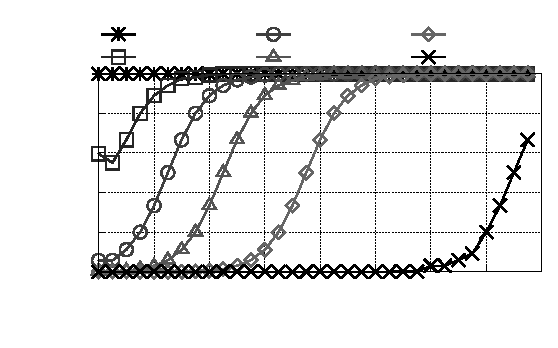
\includegraphics{modcheckout}}%
    \gplfronttext
  \end{picture}%
\endgroup
}
\caption{\Jaccard{\secretsSetSize} for different \secretsSetSize and \modulus}
\label{fig:modcheckout:Jaccard}
\end{subfigure}
%
\begin{subfigure}[b]{0.3\textwidth}
\DTLloaddb[noheader=true]{dbmodcheckout}{fig/sscf/modcheckout-0.csv}
\centering
\footnotesize{
\begin{tabular}{lcc}\toprule
\modulus & {\logSecretsSetSizeMin}& {\logSecretsSetSizeMax}\\ 
\midrule
\DTLforeach{dbmodcheckout}{\m=Column1,\nmin=Column2,\nmax=Column3}{\m & \nmin & \nmax \tabularnewline}
\\[-\normalbaselineskip]\bottomrule
\end{tabular}
}
\vspace{0.5em}
\caption{\hspace{-0.5em}\secretsSetSizeMin{} and \secretsSetSizeMax{} for different \modulus}
\label{fig:modcheckout:tbl}
\end{subfigure}
\caption{A procedure that leaks about more secrets as \modulus is decreased (see \secref{sscf:sec:micro:nmbrVsAmount})}
\label{fig:modcheckout}
\end{figure*}
\begin{figure*}
\begin{subfigure}[b]{0.26\textwidth}
\centering
\footnotesize{
\begin{tabbing}
** \= ** \= ** \= \kill
\proc(\ACIFn{}, \AIIFn{}, \SecFn{}) \\
\> $\AOOFn{}(\textrm{`result'}) \gets$ \\
\>\>\> $\SecFn{}(\secretVar) \bmod \modulus$ \\
\> return \AOOFn{} \\[7ex]
\end{tabbing}
}
\caption{Procedure\label{fig:modout:code}}
\end{subfigure}%
\begin{subfigure}[b]{0.405\textwidth}
\hspace{-1ex}
\resizebox{0.99\textwidth}{!}{\large% GNUPLOT: LaTeX picture with Postscript
\begingroup
  \fontfamily{Times-Roman}%
  \selectfont
  \makeatletter
  \providecommand\color[2][]{%
    \GenericError{(gnuplot) \space\space\space\@spaces}{%
      Package color not loaded in conjunction with
      terminal option `colourtext'%
    }{See the gnuplot documentation for explanation.%
    }{Either use 'blacktext' in gnuplot or load the package
      color.sty in LaTeX.}%
    \renewcommand\color[2][]{}%
  }%
  \providecommand\includegraphics[2][]{%
    \GenericError{(gnuplot) \space\space\space\@spaces}{%
      Package graphicx or graphics not loaded%
    }{See the gnuplot documentation for explanation.%
    }{The gnuplot epslatex terminal needs graphicx.sty or graphics.sty.}%
    \renewcommand\includegraphics[2][]{}%
  }%
  \providecommand\rotatebox[2]{#2}%
  \@ifundefined{ifGPcolor}{%
    \newif\ifGPcolor
    \GPcolortrue
  }{}%
  \@ifundefined{ifGPblacktext}{%
    \newif\ifGPblacktext
    \GPblacktexttrue
  }{}%
  % define a \g@addto@macro without @ in the name:
  \let\gplgaddtomacro\g@addto@macro
  % define empty templates for all commands taking text:
  \gdef\gplbacktext{}%
  \gdef\gplfronttext{}%
  \makeatother
  \ifGPblacktext
    % no textcolor at all
    \def\colorrgb#1{}%
    \def\colorgray#1{}%
  \else
    % gray or color?
    \ifGPcolor
      \def\colorrgb#1{\color[rgb]{#1}}%
      \def\colorgray#1{\color[gray]{#1}}%
      \expandafter\def\csname LTw\endcsname{\color{white}}%
      \expandafter\def\csname LTb\endcsname{\color{black}}%
      \expandafter\def\csname LTa\endcsname{\color{black}}%
      \expandafter\def\csname LT0\endcsname{\color[rgb]{1,0,0}}%
      \expandafter\def\csname LT1\endcsname{\color[rgb]{0,1,0}}%
      \expandafter\def\csname LT2\endcsname{\color[rgb]{0,0,1}}%
      \expandafter\def\csname LT3\endcsname{\color[rgb]{1,0,1}}%
      \expandafter\def\csname LT4\endcsname{\color[rgb]{0,1,1}}%
      \expandafter\def\csname LT5\endcsname{\color[rgb]{1,1,0}}%
      \expandafter\def\csname LT6\endcsname{\color[rgb]{0,0,0}}%
      \expandafter\def\csname LT7\endcsname{\color[rgb]{1,0.3,0}}%
      \expandafter\def\csname LT8\endcsname{\color[rgb]{0.5,0.5,0.5}}%
    \else
      % gray
      \def\colorrgb#1{\color{black}}%
      \def\colorgray#1{\color[gray]{#1}}%
      \expandafter\def\csname LTw\endcsname{\color{white}}%
      \expandafter\def\csname LTb\endcsname{\color{black}}%
      \expandafter\def\csname LTa\endcsname{\color{black}}%
      \expandafter\def\csname LT0\endcsname{\color{black}}%
      \expandafter\def\csname LT1\endcsname{\color{black}}%
      \expandafter\def\csname LT2\endcsname{\color{black}}%
      \expandafter\def\csname LT3\endcsname{\color{black}}%
      \expandafter\def\csname LT4\endcsname{\color{black}}%
      \expandafter\def\csname LT5\endcsname{\color{black}}%
      \expandafter\def\csname LT6\endcsname{\color{black}}%
      \expandafter\def\csname LT7\endcsname{\color{black}}%
      \expandafter\def\csname LT8\endcsname{\color{black}}%
    \fi
  \fi
    \setlength{\unitlength}{0.0500bp}%
    \ifx\gptboxheight\undefined%
      \newlength{\gptboxheight}%
      \newlength{\gptboxwidth}%
      \newsavebox{\gptboxtext}%
    \fi%
    \setlength{\fboxrule}{0.5pt}%
    \setlength{\fboxsep}{1pt}%
\begin{picture}(5040.00,3024.00)%
    \gplgaddtomacro\gplbacktext{%
      \csname LTb\endcsname%
      \put(694,572){\makebox(0,0)[r]{\strut{}$0$}}%
      \csname LTb\endcsname%
      \put(694,952){\makebox(0,0)[r]{\strut{}$0.2$}}%
      \csname LTb\endcsname%
      \put(694,1332){\makebox(0,0)[r]{\strut{}$0.4$}}%
      \csname LTb\endcsname%
      \put(694,1713){\makebox(0,0)[r]{\strut{}$0.6$}}%
      \csname LTb\endcsname%
      \put(694,2093){\makebox(0,0)[r]{\strut{}$0.8$}}%
      \csname LTb\endcsname%
      \put(694,2473){\makebox(0,0)[r]{\strut{}$1$}}%
      \csname LTb\endcsname%
      \put(735,396){\makebox(0,0){\strut{}$0$}}%
      \csname LTb\endcsname%
      \put(1267,396){\makebox(0,0){\strut{}$4$}}%
      \csname LTb\endcsname%
      \put(1798,396){\makebox(0,0){\strut{}$8$}}%
      \csname LTb\endcsname%
      \put(2330,396){\makebox(0,0){\strut{}$12$}}%
      \csname LTb\endcsname%
      \put(2861,396){\makebox(0,0){\strut{}$16$}}%
      \csname LTb\endcsname%
      \put(3393,396){\makebox(0,0){\strut{}$20$}}%
      \csname LTb\endcsname%
      \put(3924,396){\makebox(0,0){\strut{}$24$}}%
      \csname LTb\endcsname%
      \put(4456,396){\makebox(0,0){\strut{}$28$}}%
      \csname LTb\endcsname%
      \put(4987,396){\makebox(0,0){\strut{}$32$}}%
    }%
    \gplgaddtomacro\gplfronttext{%
      \csname LTb\endcsname%
      \put(176,1522){\rotatebox{-270}{\makebox(0,0){\strut{}\Jaccard{\secretsSetSize}}}}%
      \put(2913,154){\makebox(0,0){\strut{}$\log_2{\secretsSetSize}$}}%
      \csname LTb\endcsname%
      \put(1272,2851){\makebox(0,0)[l]{\strut{}\modulus=$1$}}%
      \csname LTb\endcsname%
      \put(1272,2631){\makebox(0,0)[l]{\strut{}\modulus=$4$}}%
      \csname LTb\endcsname%
      \put(2760,2851){\makebox(0,0)[l]{\strut{}\modulus=$64$}}%
      \csname LTb\endcsname%
      \put(2760,2631){\makebox(0,0)[l]{\strut{}\modulus=$2^{10}$}}%
      \csname LTb\endcsname%
      \put(4248,2851){\makebox(0,0)[l]{\strut{}\modulus=$2^{16}$}}%
      \csname LTb\endcsname%
      \put(4248,2631){\makebox(0,0)[l]{\strut{}\modulus=$2^{31}$}}%
    }%
    \gplbacktext
    \put(0,0){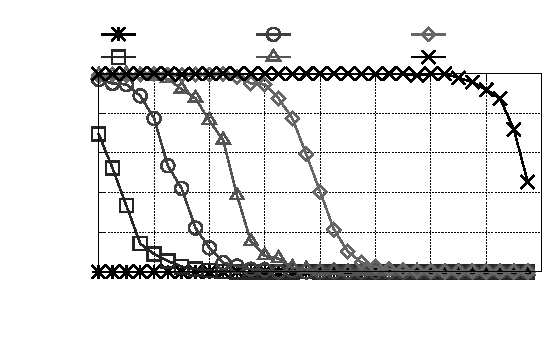
\includegraphics{modout}}%
    \gplfronttext
  \end{picture}%
\endgroup
}
\caption{\Jaccard{\secretsSetSize} for different \secretsSetSize and \modulus}
\label{fig:modout:Jaccard}
\end{subfigure}%
\begin{subfigure}[b]{0.3\textwidth}
\footnotesize{
\DTLloaddb[noheader=true]{dbmodout}{fig/sscf/modout-0.csv}
\centering
\begin{tabular}{lcc}\toprule
\modulus & {\logSecretsSetSizeMin}& {\logSecretsSetSizeMax}\\ 
\midrule
\DTLforeach{dbmodout}{\m=Column1,\nmin=Column2,\nmax=Column3}{\m & \nmin & \nmax \tabularnewline}
\\[-\normalbaselineskip]\bottomrule
\multicolumn{3}{l}{\parbox{0.95\linewidth}{\scriptsize``nan'' denotes
    ``not a number,'' i.e., $\secretsSetSizeMin{} = 0$ or
    $\secretsSetSizeMax{} = 0$}}
\end{tabular}
}
\vspace{0.5em}
\caption{\hspace{-0.5em}\secretsSetSizeMin{} and \secretsSetSizeMax{} for different \modulus}
\label{fig:modout:tbl}
\end{subfigure}
\caption{A procedure that leaks more about secret values as \modulus is increased (see \secref{sscf:sec:micro:nmbrVsAmount})}
\label{fig:modout}
\end{figure*}

In \secref{sscf:sec:measurement:secretsSetSize}, we showed through an
idealized example how a small \secretsSetSize is more useful for
evaluating the number of secrets about which information leaks,
whereas a large \secretsSetSize is more useful for evaluating the
amount of information leaked about these secrets.  Now we will use two
simple procedures with a controllable constant \modulus to
quantitatively demonstrate the necessity of varying \secretsSetSize
and the correct usage of \secretsSetSizeMin{} and
\secretsSetSizeMax{}.

The first procedure, shown in \figref{fig:modcheckout:code}, returns
the secret value if it is divisible by a constant $\modulus$ and
returns zero otherwise, where both $\SecFn{}(\secretVar)$ and \modulus
are 32-bit integers.  This procedure leaks the same amount of
information (the whole secret) about a larger number of secret values
if \modulus is decreased.  The behavior of \Jaccard{\secretsSetSize}
shown in \figref{fig:modcheckout:Jaccard} is consistent with this
observation.  Specifically, different values of \modulus induce curves
for \Jaccard{\secretsSetSize} that differ primarily in the minimum
value of \secretsSetSize where \Jaccard{\secretsSetSize} is large.
This behavior is also seen in the value of \secretsSetSizeMin{} in
\figref{fig:modcheckout:tbl}, where \secretsSetSizeMin{} ranges from
$\secretsSetSizeMin{} \approx 0$ at $\modulus = 2^{31}$ to
$\secretsSetSizeMin{} = 1$ at $\modulus = 1$.

Contrast this case with the procedure shown in
\figref{fig:modout:code}, which returns the residue class of the
secret value modulo a constant value \modulus.  As such, as \modulus
is increased, more information about each secret is leaked.  This is
demonstrated in \figref{fig:modout:Jaccard}, where the curves for
different values of \modulus differ in primarily in the maximum value
\secretsSetSize at which \Jaccard{\secretsSetSize} is large.
Similarly, \secretsSetSizeMax{} ranges from $\secretsSetSizeMax{} = 0$
at $\modulus = 1$ to $\secretsSetSizeMax{} \approx
2^{-0.8} \approx 0.57$ at $\modulus = 2^{31}$.

An example that blends these the previous two examples is show in in
\figref{fig:modcheck:code}; here the procedure returns $1$ if
$\SecFn{}(\secretVar) \bmod \modulus = \ACIFn{}(\textrm{`test'})$ and
$0$ otherwise, where \modulus is a 32-bit constant.  As such, this
procedure leaks a lot about a few secret values when \modulus is
large, and a little about many secret values when \modulus is small.
As shown in the $\roundNmbr=1$ columns of \figref{fig:modcheck:tbl},
\secretsSetSizeMin{} and \secretsSetSizeMax{} monotonically decreases
and increase, respectively, as \modulus grows.

\subsection{Leaking more over multiple rounds}
\label{sscf:sec:micro:rounds}
\begin{figure}[tb]
\begin{subfigure}[b]{0.4\textwidth}
\centering{\small
\begin{tabbing}
** \= ** \= ***** \= \kill
\proc(\ACIFn{}, \AIIFn{}, \SecFn{}) \\
\> if ($\SecFn{}(\secretVar) \bmod\modulus=\ACIFn{}(\textrm{`test'})$) \\
\> \> $\AOOFn{}(\textrm{`result'}) \gets 1$ \\
\> else \\
\> \> $\AOOFn{}(\textrm{`result'}) \gets 0$ \\
\> return \AOOFn{} \\[0.5ex]
\end{tabbing}
}
\caption{Procedure\label{fig:modcheck:code}}
\end{subfigure}
\begin{subfigure}[b]{0.5\textwidth}
\centering
\resizebox{1\textwidth}{!}{\large{% GNUPLOT: LaTeX picture with Postscript
\begingroup
  \fontfamily{Times-Roman}%
  \selectfont
  \makeatletter
  \providecommand\color[2][]{%
    \GenericError{(gnuplot) \space\space\space\@spaces}{%
      Package color not loaded in conjunction with
      terminal option `colourtext'%
    }{See the gnuplot documentation for explanation.%
    }{Either use 'blacktext' in gnuplot or load the package
      color.sty in LaTeX.}%
    \renewcommand\color[2][]{}%
  }%
  \providecommand\includegraphics[2][]{%
    \GenericError{(gnuplot) \space\space\space\@spaces}{%
      Package graphicx or graphics not loaded%
    }{See the gnuplot documentation for explanation.%
    }{The gnuplot epslatex terminal needs graphicx.sty or graphics.sty.}%
    \renewcommand\includegraphics[2][]{}%
  }%
  \providecommand\rotatebox[2]{#2}%
  \@ifundefined{ifGPcolor}{%
    \newif\ifGPcolor
    \GPcolortrue
  }{}%
  \@ifundefined{ifGPblacktext}{%
    \newif\ifGPblacktext
    \GPblacktexttrue
  }{}%
  % define a \g@addto@macro without @ in the name:
  \let\gplgaddtomacro\g@addto@macro
  % define empty templates for all commands taking text:
  \gdef\gplbacktext{}%
  \gdef\gplfronttext{}%
  \makeatother
  \ifGPblacktext
    % no textcolor at all
    \def\colorrgb#1{}%
    \def\colorgray#1{}%
  \else
    % gray or color?
    \ifGPcolor
      \def\colorrgb#1{\color[rgb]{#1}}%
      \def\colorgray#1{\color[gray]{#1}}%
      \expandafter\def\csname LTw\endcsname{\color{white}}%
      \expandafter\def\csname LTb\endcsname{\color{black}}%
      \expandafter\def\csname LTa\endcsname{\color{black}}%
      \expandafter\def\csname LT0\endcsname{\color[rgb]{1,0,0}}%
      \expandafter\def\csname LT1\endcsname{\color[rgb]{0,1,0}}%
      \expandafter\def\csname LT2\endcsname{\color[rgb]{0,0,1}}%
      \expandafter\def\csname LT3\endcsname{\color[rgb]{1,0,1}}%
      \expandafter\def\csname LT4\endcsname{\color[rgb]{0,1,1}}%
      \expandafter\def\csname LT5\endcsname{\color[rgb]{1,1,0}}%
      \expandafter\def\csname LT6\endcsname{\color[rgb]{0,0,0}}%
      \expandafter\def\csname LT7\endcsname{\color[rgb]{1,0.3,0}}%
      \expandafter\def\csname LT8\endcsname{\color[rgb]{0.5,0.5,0.5}}%
    \else
      % gray
      \def\colorrgb#1{\color{black}}%
      \def\colorgray#1{\color[gray]{#1}}%
      \expandafter\def\csname LTw\endcsname{\color{white}}%
      \expandafter\def\csname LTb\endcsname{\color{black}}%
      \expandafter\def\csname LTa\endcsname{\color{black}}%
      \expandafter\def\csname LT0\endcsname{\color{black}}%
      \expandafter\def\csname LT1\endcsname{\color{black}}%
      \expandafter\def\csname LT2\endcsname{\color{black}}%
      \expandafter\def\csname LT3\endcsname{\color{black}}%
      \expandafter\def\csname LT4\endcsname{\color{black}}%
      \expandafter\def\csname LT5\endcsname{\color{black}}%
      \expandafter\def\csname LT6\endcsname{\color{black}}%
      \expandafter\def\csname LT7\endcsname{\color{black}}%
      \expandafter\def\csname LT8\endcsname{\color{black}}%
    \fi
  \fi
    \setlength{\unitlength}{0.0500bp}%
    \ifx\gptboxheight\undefined%
      \newlength{\gptboxheight}%
      \newlength{\gptboxwidth}%
      \newsavebox{\gptboxtext}%
    \fi%
    \setlength{\fboxrule}{0.5pt}%
    \setlength{\fboxsep}{1pt}%
\begin{picture}(5040.00,3024.00)%
    \gplgaddtomacro\gplbacktext{%
      \csname LTb\endcsname%
      \put(633,550){\makebox(0,0)[r]{\strut{}$0$}}%
      \csname LTb\endcsname%
      \put(633,1328){\makebox(0,0)[r]{\strut{}$0.2$}}%
      \csname LTb\endcsname%
      \put(633,2105){\makebox(0,0)[r]{\strut{}$0.4$}}%
      \csname LTb\endcsname%
      \put(726,352){\makebox(0,0){\strut{}$0$}}%
      \csname LTb\endcsname%
      \put(1265,352){\makebox(0,0){\strut{}$4$}}%
      \csname LTb\endcsname%
      \put(1804,352){\makebox(0,0){\strut{}$8$}}%
      \csname LTb\endcsname%
      \put(2343,352){\makebox(0,0){\strut{}$12$}}%
      \csname LTb\endcsname%
      \put(2883,352){\makebox(0,0){\strut{}$16$}}%
      \csname LTb\endcsname%
      \put(3422,352){\makebox(0,0){\strut{}$20$}}%
      \csname LTb\endcsname%
      \put(3961,352){\makebox(0,0){\strut{}$24$}}%
      \csname LTb\endcsname%
      \put(4500,352){\makebox(0,0){\strut{}$28$}}%
      \csname LTb\endcsname%
      \put(5039,352){\makebox(0,0){\strut{}$32$}}%
    }%
    \gplgaddtomacro\gplfronttext{%
      \csname LTb\endcsname%
      \put(88,1522){\rotatebox{-270}{\makebox(0,0){\strut{}\Jaccard{\secretsSetSize}}}}%
      \put(2882,110){\makebox(0,0){\strut{}$\log_2{\secretsSetSize}$}}%
      \csname LTb\endcsname%
      \put(720,2851){\makebox(0,0)[l]{\strut{}\modulus=$2$}}%
      \csname LTb\endcsname%
      \put(720,2631){\makebox(0,0)[l]{\strut{}\modulus=$4$}}%
      \csname LTb\endcsname%
      \put(1931,2851){\makebox(0,0)[l]{\strut{}\modulus=$8$}}%
      \csname LTb\endcsname%
      \put(1931,2631){\makebox(0,0)[l]{\strut{}\modulus=$64$}}%
      \csname LTb\endcsname%
      \put(3142,2851){\makebox(0,0)[l]{\strut{}\modulus=$2^{10}$}}%
      \csname LTb\endcsname%
      \put(3142,2631){\makebox(0,0)[l]{\strut{}\modulus=$2^{29}$}}%
      \csname LTb\endcsname%
      \put(4353,2851){\makebox(0,0)[l]{\strut{}\modulus=$2^{31}$}}%
    }%
    \gplbacktext
    \put(0,0){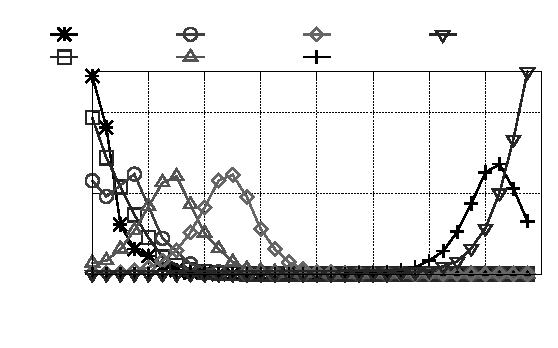
\includegraphics{modcheck}}%
    \gplfronttext
  \end{picture}%
\endgroup
}}
\caption{\Jaccard{\secretsSetSize} for different \secretsSetSize}
\label{fig:modcheck:Jaccard}
\end{subfigure}\\
\begin{subfigure}[b]{\textwidth}
\centering
{\small	
\setlength\tabcolsep{0.1em}
\DTLloaddb[noheader=true]{dbmodcheck1}{fig/sscf/modcheck-1.csv}
\DTLloaddb[noheader=true]{dbmodcheck2}{fig/sscf/modcheck-2.csv}
\begin{tabular}{lrrrrrrrr}
\toprule
\multirow{2}{*}{\modulus}& \multicolumn{4}{c}{\logSecretsSetSizeMin}& \multicolumn{4}{c}{\logSecretsSetSizeMax}\\ \cline{2-9}
& $\roundNmbr=1$ & $\roundNmbr=2$ & $\roundNmbr=4$ & $\roundNmbr=6$ & $\roundNmbr=1$ & $\roundNmbr=2$ & $\roundNmbr=4$ & $\roundNmbr=6$ \\
\midrule
\DTLforeach{dbmodcheck1}{\m=Column1,\nminone=Column2,\nmintwo=Column3,\nminfour=Column4,\nminsix=Column5}{%
\DTLforeach[\DTLiseq{\mm}{\m}]{dbmodcheck2}{\mm=Column1,\nmaxone=Column2,\nmaxtwo=Column3,\nmaxfour=Column4,\nmaxsix=Column5}{
\m &\nminone&\nmintwo& \nminfour& \nminsix& \nmaxone& \nmaxtwo
	&\nmaxfour& \nmaxsix \tabularnewline%
}}
 \\[-\normalbaselineskip]\bottomrule
\end{tabular}
}
\vspace{0.5em}
\caption{\secretsSetSizeMin{} and \secretsSetSizeMax{} for different \modulus\label{fig:modcheck:tbl}}
\end{subfigure}
\caption{Leakage of procedure that checks a guess of secret's residue class modulo \modulus (see \secrefs{sscf:sec:micro:nmbrVsAmount}{sscf:sec:micro:rounds})}
\label{fig:modcheck}
\end{figure}
A second way to view the example in \figref{fig:modcheck} is to
consider \roundNmbr procedure executions using the same
$\SecFn{}(\secretVar)$ (i.e., $\SecFn{1}(\secretVar)$ $=$
$\SecFn{2}(\secretVar)$ $=$ $\ldots$ $=$
$\SecFn{\roundNmbr}(\secretVar)$).  Our intuition suggests that after
$\roundNmbr = \modulus-1$ executions of the procedure, a smart
attacker will have learned everything about $\SecFn{}(\secretVar)$
that it can from \proc; e.g., by setting
$\ACIFn{\roundIdx}(\textrm{`test'}) = \roundIdx$, the attacker either
will have observed some $\AOOFn{\roundIdx}(\textrm{`result'}) = 1$, in
which case it knows $\SecFn{}(\secretVar) \bmod \modulus = \roundIdx$,
or else it knows $\SecFn{}(\secretVar) \bmod \modulus = 0$.
Consistent with that intuition, in \figref{fig:modcheck:tbl}, both
\secretsSetSizeMin{} and \secretsSetSizeMax{} remain steady for
$\modulus = 2$ as \roundNmbr increases, since no new information is
available to the attacker after $\roundNmbr=1$. Similarly, for
$\modulus = 4$, $\secretsSetSizeMin{}$ and $\secretsSetSizeMax{}$ both
increase precipitously (by $\ge 74\%$) from $\roundNmbr=1$ to
$\roundNmbr=2$ and then begin to flatten out (albeit
imperfectly---both are estimated values, after all), which is
consistent with this intuition that the attacker should learn no new
information past $\roundNmbr = 3$.  For $\modulus > 4$, each
additional procedure execution provides additional information to the
attacker about all secrets and much more about some (namely those for
which it learns the residue class mod \modulus).  Correspondingly,
both \secretsSetSizeMin{} and \secretsSetSizeMax{} increase
monotonically along each of these rows.

\subsection{Leaking the secret conditioned on randomness}
\label{sscf:sec:micro:random}
We now illustrate the ability of our technique to measure leakage from
a different randomized procedure from that discussed in
\figref{fig:inflating}.  The procedure, shown in
\figref{fig:randout:code}, returns the secret if a random value is
divisible by a constant \modulus and returns that random value
otherwise.  Clearly, a larger \modulus implies that fewer secret
values leak, but those that leak do so completely.  This behavior is
illustrated by the \JaccardRand{\secretsSetSize} measure shown in
\figref{fig:randout:Jaccard}; the leakage is consistently higher for
lower values of \modulus.  Similarly, while \secretsSetSizeMaxRand{}
remains high for all values of \modulus (never dropping below
$\frac{1}{4}$), \secretsSetSizeMinRand{} ranges from
$\secretsSetSizeMinRand{} = 1$ when all secrets are leaked ($\modulus
= 1$) to $\secretsSetSizeMinRand{} \approx 0$ when few secrets are
leaked ($\modulus = 2^{31}$).
\begin{figure}[tb]
\begin{subfigure}[b]{0.28\textwidth}
\centering
{\small
\begin{tabbing}
** \= ** \= \kill
\proc(\ACIFn{},\AIIFn{},\SecFn{}) \\
\>  if ($\AIIFn{}(\textrm{`rand'}) \bmod \modulus = 0$) \\
\> \> $\AOOFn{}(\textrm{`result'}) \gets \SecFn{}(\secretVar)$ \\
\>  else \\
\> \>  $\AOOFn{}(\textrm{`result'}) \gets \AIIFn{}(\textrm{`rand'})$ \\
\> return \AOOFn{} \\[2ex]
\end{tabbing}
}
\caption{Procedure}
\label{fig:randout:code}
\end{subfigure}
\hspace{-2ex}
\begin{subfigure}[b]{0.38\textwidth}
\centering
\resizebox{0.95\textwidth}{!}{\large% GNUPLOT: LaTeX picture with Postscript
\begingroup
  \fontfamily{Times-Roman}%
  \selectfont
  \makeatletter
  \providecommand\color[2][]{%
    \GenericError{(gnuplot) \space\space\space\@spaces}{%
      Package color not loaded in conjunction with
      terminal option `colourtext'%
    }{See the gnuplot documentation for explanation.%
    }{Either use 'blacktext' in gnuplot or load the package
      color.sty in LaTeX.}%
    \renewcommand\color[2][]{}%
  }%
  \providecommand\includegraphics[2][]{%
    \GenericError{(gnuplot) \space\space\space\@spaces}{%
      Package graphicx or graphics not loaded%
    }{See the gnuplot documentation for explanation.%
    }{The gnuplot epslatex terminal needs graphicx.sty or graphics.sty.}%
    \renewcommand\includegraphics[2][]{}%
  }%
  \providecommand\rotatebox[2]{#2}%
  \@ifundefined{ifGPcolor}{%
    \newif\ifGPcolor
    \GPcolortrue
  }{}%
  \@ifundefined{ifGPblacktext}{%
    \newif\ifGPblacktext
    \GPblacktexttrue
  }{}%
  % define a \g@addto@macro without @ in the name:
  \let\gplgaddtomacro\g@addto@macro
  % define empty templates for all commands taking text:
  \gdef\gplbacktext{}%
  \gdef\gplfronttext{}%
  \makeatother
  \ifGPblacktext
    % no textcolor at all
    \def\colorrgb#1{}%
    \def\colorgray#1{}%
  \else
    % gray or color?
    \ifGPcolor
      \def\colorrgb#1{\color[rgb]{#1}}%
      \def\colorgray#1{\color[gray]{#1}}%
      \expandafter\def\csname LTw\endcsname{\color{white}}%
      \expandafter\def\csname LTb\endcsname{\color{black}}%
      \expandafter\def\csname LTa\endcsname{\color{black}}%
      \expandafter\def\csname LT0\endcsname{\color[rgb]{1,0,0}}%
      \expandafter\def\csname LT1\endcsname{\color[rgb]{0,1,0}}%
      \expandafter\def\csname LT2\endcsname{\color[rgb]{0,0,1}}%
      \expandafter\def\csname LT3\endcsname{\color[rgb]{1,0,1}}%
      \expandafter\def\csname LT4\endcsname{\color[rgb]{0,1,1}}%
      \expandafter\def\csname LT5\endcsname{\color[rgb]{1,1,0}}%
      \expandafter\def\csname LT6\endcsname{\color[rgb]{0,0,0}}%
      \expandafter\def\csname LT7\endcsname{\color[rgb]{1,0.3,0}}%
      \expandafter\def\csname LT8\endcsname{\color[rgb]{0.5,0.5,0.5}}%
    \else
      % gray
      \def\colorrgb#1{\color{black}}%
      \def\colorgray#1{\color[gray]{#1}}%
      \expandafter\def\csname LTw\endcsname{\color{white}}%
      \expandafter\def\csname LTb\endcsname{\color{black}}%
      \expandafter\def\csname LTa\endcsname{\color{black}}%
      \expandafter\def\csname LT0\endcsname{\color{black}}%
      \expandafter\def\csname LT1\endcsname{\color{black}}%
      \expandafter\def\csname LT2\endcsname{\color{black}}%
      \expandafter\def\csname LT3\endcsname{\color{black}}%
      \expandafter\def\csname LT4\endcsname{\color{black}}%
      \expandafter\def\csname LT5\endcsname{\color{black}}%
      \expandafter\def\csname LT6\endcsname{\color{black}}%
      \expandafter\def\csname LT7\endcsname{\color{black}}%
      \expandafter\def\csname LT8\endcsname{\color{black}}%
    \fi
  \fi
    \setlength{\unitlength}{0.0500bp}%
    \ifx\gptboxheight\undefined%
      \newlength{\gptboxheight}%
      \newlength{\gptboxwidth}%
      \newsavebox{\gptboxtext}%
    \fi%
    \setlength{\fboxrule}{0.5pt}%
    \setlength{\fboxsep}{1pt}%
\begin{picture}(5040.00,2880.00)%
    \gplgaddtomacro\gplbacktext{%
      \csname LTb\endcsname%
      \put(694,418){\makebox(0,0)[r]{\strut{}$0$}}%
      \csname LTb\endcsname%
      \put(694,800){\makebox(0,0)[r]{\strut{}$0.2$}}%
      \csname LTb\endcsname%
      \put(694,1182){\makebox(0,0)[r]{\strut{}$0.4$}}%
      \csname LTb\endcsname%
      \put(694,1565){\makebox(0,0)[r]{\strut{}$0.6$}}%
      \csname LTb\endcsname%
      \put(694,1947){\makebox(0,0)[r]{\strut{}$0.8$}}%
      \csname LTb\endcsname%
      \put(694,2329){\makebox(0,0)[r]{\strut{}$1$}}%
      \csname LTb\endcsname%
      \put(787,242){\makebox(0,0){\strut{}$0$}}%
      \csname LTb\endcsname%
      \put(1319,242){\makebox(0,0){\strut{}$4$}}%
      \csname LTb\endcsname%
      \put(1850,242){\makebox(0,0){\strut{}$8$}}%
      \csname LTb\endcsname%
      \put(2382,242){\makebox(0,0){\strut{}$12$}}%
      \csname LTb\endcsname%
      \put(2913,242){\makebox(0,0){\strut{}$16$}}%
      \csname LTb\endcsname%
      \put(3445,242){\makebox(0,0){\strut{}$20$}}%
      \csname LTb\endcsname%
      \put(3976,242){\makebox(0,0){\strut{}$24$}}%
      \csname LTb\endcsname%
      \put(4508,242){\makebox(0,0){\strut{}$28$}}%
      \csname LTb\endcsname%
      \put(5039,242){\makebox(0,0){\strut{}$32$}}%
    }%
    \gplgaddtomacro\gplfronttext{%
      \csname LTb\endcsname%
      \put(176,1373){\rotatebox{-270}{\makebox(0,0){\strut{}\JaccardRand{\secretsSetSize}}}}%
      \put(2913,44){\makebox(0,0){\strut{}$\log_2{\secretsSetSize}$}}%
      \csname LTb\endcsname%
      \put(1429,2707){\makebox(0,0)[l]{\strut{}\modulus=$1$}}%
      \csname LTb\endcsname%
      \put(1429,2487){\makebox(0,0)[l]{\strut{}\modulus=$2$}}%
      \csname LTb\endcsname%
      \put(2812,2707){\makebox(0,0)[l]{\strut{}\modulus=$4$}}%
      \csname LTb\endcsname%
      \put(2812,2487){\makebox(0,0)[l]{\strut{}\modulus=$64$}}%
      \csname LTb\endcsname%
      \put(4195,2707){\makebox(0,0)[l]{\strut{}\modulus=$2^{10}$}}%
      \csname LTb\endcsname%
      \put(4195,2487){\makebox(0,0)[l]{\strut{}\modulus=$2^{31}$}}%
    }%
    \gplbacktext
    \put(0,0){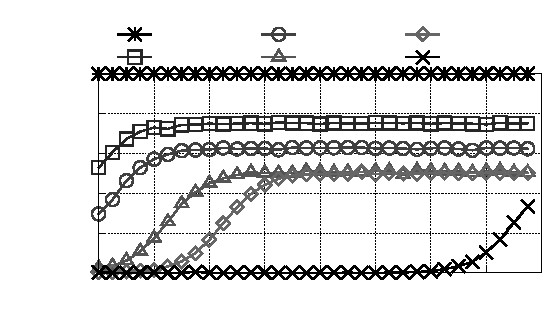
\includegraphics{randout}}%
    \gplfronttext
  \end{picture}%
\endgroup
}
\caption{\JaccardRand{\secretsSetSize} for different \secretsSetSize and \modulus}
\label{fig:randout:Jaccard}
\end{subfigure}
\hspace{-2ex}
\begin{subfigure}[b]{0.3\textwidth}
\centering\small{
\DTLloaddb[noheader=true,headers={\modulus,$\log_1{\secretsSetSizeMinRand{}}$,$\log_2{\secretsSetSizeMaxRand{}}$}]{dbrandout}{fig/sscf/randout-0.csv}
\centering
\renewcommand{\arraystretch}{1}
\begin{tabular}{lcc}\toprule
\modulus & \logSecretsSetSizeMinRand & \logSecretsSetSizeMaxRand \\ 
\midrule
\DTLforeach{dbrandout}{\m=Column1,\nmin=Column2,\nmax=Column3}{\m & \nmin & \nmax \tabularnewline}
 \\[-\normalbaselineskip]\bottomrule
\end{tabular}
}
\vspace{0.5em}
\caption{\secretsSetSizeMinRand{} and \secretsSetSizeMaxRand{} for different \modulus}
\label{fig:randout:sumJaccard}
\end{subfigure}
\caption{An example illustrating leakage dependent on randomness (see \secref{sscf:sec:micro:random})}
\label{fig:randout}
\end{figure}


\section{Case Studies}
\label{sscf:sec:case-studies}

In this section, we illustrate our measurement by applying it to
real-world codebases susceptible to the inference of search queries
via packet-size observations, inference of secret values due to
compression results, and inference of TCP sequence numbers.  We claim
no novelty in identifying these attacks; all are known and explored in
other papers, though not in the particular codebases (or codebase
versions) that we examine here and typically only through
application-specific analysis.  Our contribution lies in showing the
applications of our methodology to measuring interference in an
application-agnostic way and the impact of alternatives for mitigating
that interference.

\subsection{Traffic analysis on web applications}
\label{sscf:sec:case-studies:sphinx}
\begin{figure}[tb]
\begin{subfigure}[b]{\textwidth}
\centering
\small
 \setlength\tabcolsep{0.3ex}
  \DTLloaddb[headers={Keyword,Trigrams}]{myDB}{fig/sscf/sphinx.csv}
  {\DTLdisplaydb{myDB}}
  \caption{Small database for \sphinx}
  \label{fig:sphinx:db}
\end{subfigure}\\
\begin{subfigure}[b]{0.6\linewidth}
\hspace{-2ex}
 \resizebox{0.9\textwidth}{!}{\protect\small% GNUPLOT: LaTeX picture with Postscript
\begingroup
  \fontfamily{Times-Roman}%
  \selectfont
  \makeatletter
  \providecommand\color[2][]{%
    \GenericError{(gnuplot) \space\space\space\@spaces}{%
      Package color not loaded in conjunction with
      terminal option `colourtext'%
    }{See the gnuplot documentation for explanation.%
    }{Either use 'blacktext' in gnuplot or load the package
      color.sty in LaTeX.}%
    \renewcommand\color[2][]{}%
  }%
  \providecommand\includegraphics[2][]{%
    \GenericError{(gnuplot) \space\space\space\@spaces}{%
      Package graphicx or graphics not loaded%
    }{See the gnuplot documentation for explanation.%
    }{The gnuplot epslatex terminal needs graphicx.sty or graphics.sty.}%
    \renewcommand\includegraphics[2][]{}%
  }%
  \providecommand\rotatebox[2]{#2}%
  \@ifundefined{ifGPcolor}{%
    \newif\ifGPcolor
    \GPcolortrue
  }{}%
  \@ifundefined{ifGPblacktext}{%
    \newif\ifGPblacktext
    \GPblacktexttrue
  }{}%
  % define a \g@addto@macro without @ in the name:
  \let\gplgaddtomacro\g@addto@macro
  % define empty templates for all commands taking text:
  \gdef\gplbacktext{}%
  \gdef\gplfronttext{}%
  \makeatother
  \ifGPblacktext
    % no textcolor at all
    \def\colorrgb#1{}%
    \def\colorgray#1{}%
  \else
    % gray or color?
    \ifGPcolor
      \def\colorrgb#1{\color[rgb]{#1}}%
      \def\colorgray#1{\color[gray]{#1}}%
      \expandafter\def\csname LTw\endcsname{\color{white}}%
      \expandafter\def\csname LTb\endcsname{\color{black}}%
      \expandafter\def\csname LTa\endcsname{\color{black}}%
      \expandafter\def\csname LT0\endcsname{\color[rgb]{1,0,0}}%
      \expandafter\def\csname LT1\endcsname{\color[rgb]{0,1,0}}%
      \expandafter\def\csname LT2\endcsname{\color[rgb]{0,0,1}}%
      \expandafter\def\csname LT3\endcsname{\color[rgb]{1,0,1}}%
      \expandafter\def\csname LT4\endcsname{\color[rgb]{0,1,1}}%
      \expandafter\def\csname LT5\endcsname{\color[rgb]{1,1,0}}%
      \expandafter\def\csname LT6\endcsname{\color[rgb]{0,0,0}}%
      \expandafter\def\csname LT7\endcsname{\color[rgb]{1,0.3,0}}%
      \expandafter\def\csname LT8\endcsname{\color[rgb]{0.5,0.5,0.5}}%
    \else
      % gray
      \def\colorrgb#1{\color{black}}%
      \def\colorgray#1{\color[gray]{#1}}%
      \expandafter\def\csname LTw\endcsname{\color{white}}%
      \expandafter\def\csname LTb\endcsname{\color{black}}%
      \expandafter\def\csname LTa\endcsname{\color{black}}%
      \expandafter\def\csname LT0\endcsname{\color{black}}%
      \expandafter\def\csname LT1\endcsname{\color{black}}%
      \expandafter\def\csname LT2\endcsname{\color{black}}%
      \expandafter\def\csname LT3\endcsname{\color{black}}%
      \expandafter\def\csname LT4\endcsname{\color{black}}%
      \expandafter\def\csname LT5\endcsname{\color{black}}%
      \expandafter\def\csname LT6\endcsname{\color{black}}%
      \expandafter\def\csname LT7\endcsname{\color{black}}%
      \expandafter\def\csname LT8\endcsname{\color{black}}%
    \fi
  \fi
    \setlength{\unitlength}{0.0500bp}%
    \ifx\gptboxheight\undefined%
      \newlength{\gptboxheight}%
      \newlength{\gptboxwidth}%
      \newsavebox{\gptboxtext}%
    \fi%
    \setlength{\fboxrule}{0.5pt}%
    \setlength{\fboxsep}{1pt}%
\begin{picture}(4608.00,2590.00)%
    \gplgaddtomacro\gplbacktext{%
      \csname LTb\endcsname%
      \put(524,368){\makebox(0,0)[r]{\strut{}$0$}}%
      \csname LTb\endcsname%
      \put(524,938){\makebox(0,0)[r]{\strut{}$0.2$}}%
      \csname LTb\endcsname%
      \put(524,1507){\makebox(0,0)[r]{\strut{}$0.4$}}%
      \csname LTb\endcsname%
      \put(524,2077){\makebox(0,0)[r]{\strut{}$0.6$}}%
      \csname LTb\endcsname%
      \put(572,240){\makebox(0,0){\strut{}$0$}}%
      \csname LTb\endcsname%
      \put(1722,240){\makebox(0,0){\strut{}$4$}}%
      \csname LTb\endcsname%
      \put(2872,240){\makebox(0,0){\strut{}$8$}}%
      \csname LTb\endcsname%
      \put(4022,240){\makebox(0,0){\strut{}$12$}}%
    }%
    \gplgaddtomacro\gplfronttext{%
      \csname LTb\endcsname%
      \put(128,1254){\rotatebox{-270}{\makebox(0,0){\strut{}\JaccardRand{\secretsSetSize}}}}%
      \put(2584,32){\makebox(0,0){\strut{}$\lceil\log_{2}{\secretsSetSize}\rceil$}}%
      \csname LTb\endcsname%
      \put(841,2423){\makebox(0,0)[l]{\strut{}rand.2}}%
      \csname LTb\endcsname%
      \put(841,2215){\makebox(0,0)[l]{\strut{}fix.64}}%
      \csname LTb\endcsname%
      \put(1912,2423){\makebox(0,0)[l]{\strut{}rand.16}}%
      \csname LTb\endcsname%
      \put(1912,2215){\makebox(0,0)[l]{\strut{}fix.256}}%
      \csname LTb\endcsname%
      \put(2983,2423){\makebox(0,0)[l]{\strut{}rand.64}}%
      \csname LTb\endcsname%
      \put(2983,2215){\makebox(0,0)[l]{\strut{}nopadding}}%
      \csname LTb\endcsname%
      \put(4054,2423){\makebox(0,0)[l]{\strut{}rand.128}}%
    }%
    \gplbacktext
    \put(0,0){\includegraphics{sphinx}}%
    \gplfronttext
  \end{picture}%
\endgroup
}
  %\includegraphics[width=\linewidth]{fig/sscf/sphinx.eps}
\vspace{1ex}
  \caption{\JaccardRand{\secretsSetSize} for different \secretsSetSize}
  \label{fig:sphinx:JaccardRand}
\end{subfigure}
\begin{subfigure}[b]{0.4\linewidth}
  \centering
{\small  
  \DTLloaddb[noheader=true]{sphinxresult}{fig/sscf/sphinx-0.csv}
 \setlength\tabcolsep{0.4ex}
\begin{tabular}{lcc}\toprule
Mitigation & {$\log_2{\secretsSetSizeMinRand{}}$}& {$\log_2{\secretsSetSizeMaxRand{}}$}\\ 
\midrule
\DTLforeach{sphinxresult}{\m=Column1,\nmin=Column2,\nmax=Column3}{%
	\textrm{\m} & \nmin & \nmax \tabularnewline%
}
\\[-1.1\normalbaselineskip]\bottomrule
\multicolumn{3}{l}{\parbox{0.9\linewidth}{\vspace{0.1\normalbaselineskip}
    \scriptsize``nan'' denotes ``not a number,'' i.e.,
    $\secretsSetSizeMinRand{} = 0$ or $\secretsSetSizeMaxRand{} = 0$}}
\end{tabular}
}
\vspace{1ex}
\caption{\secretsSetSizeMinRand{} and \secretsSetSizeMaxRand{} for different mitigations}
\label{fig:sphinx:tbl}
\end{subfigure}
\caption[Analysis of auto-complete feature]{Analysis of auto-complete feature of \sphinx and mitigation strategies (see \secref{sscf:sec:case-studies:sphinx})}
\label{fig:sphinx}
\end{figure}
Packet sizes are a known side channel for reverse engineering search
queries and other web content returned from a server, and defenses
against this side channel have been studied using various methods of
\QIF
(e.g.,~\cite{Kellaris:2016:GAS:2976749.2978386,sidebuster:ccs10,webTomorrow:sp10}).
Specifically, a network attacker can often distinguish between two
queries to a web search engine because the response traffic length is
dependent on the query.  Even packet padding may not hide all secret
information~\cite{trafficcounter}.

In this section, we use our methodology to analyze the auto-complete
feature of search engines to demonstrate our ability to detect the
leakage of the user's query from the network packet sizes.
Furthermore, we repeat our analysis after applying mitigations
suggested in previous work~\cite{trafficcounter}.  This allows us to
compare the effectiveness of these mitigations to the original
implementation.

We evaluated a C++ web server called \sphinx
(\url{http://sphinxsearch.com/}), which provides PHP APIs for a client
to send a query string to the server.  The auto-complete feature then
returns a list of keywords that best match the query string.  To
generate the postcondition that characterizes the auto-complete
feature, we marked the query string as the secret (i.e.,
$\SecFn{}(\secretVar)$ is the query string) and the final application
response length as the observable (i.e., $\AOOKeys =
\{\textrm{`\textrm{response\_length}'}\}$), by injecting only two
lines into the server's code.  In this application, there was no
attacker-controlled input and no other input (i.e., $\ACIKeys =
\AIIKeys = \emptyset$).

Since the auto-complete results depend on the contents of the server
database, we simply instantiated the database with an example
containing six keywords and 35 query trigrams (see
\figref{fig:sphinx:db}).  When provided an input query string of at
least three characters, \sphinx returns (content containing) the two
keywords with the highest ``score'' based on matching trigrams in the
query string to each keyword's associated trigrams.  We also limited
queries to three characters drawn from $\{\textrm{`a'}, \ldots,
\textrm{`z'}\}$ ($\{97,\ldots,122\}$ in ASCII), yielding $26^3 \approx
2^{14}$ possible queries.  Note that instantiating the server with a
specific database and limiting the query characters and length as
described cannot induce our analysis to provide false positives,
though it can contribute false negatives.

We experimented with two types of mitigation strategies.
\textit{Random padding} is motivated by protocols like SSH that
obfuscate traffic lengths by adding a random amount of padding up to
some maximum limit to the application response payload.  We
experimented with padding lengths of up to 2 bytes (`rand.2'), 16
bytes (`rand.16'), 64 bytes (`rand.64'), and 128 bytes
(`rand.128').  \textit{Padding to a fixed length} is a second
strategy, which increases the length of the application response
payload to the nearest multiple of a fixed length.  We experimented
with padding to a multiple of 64 bytes (`fixed.64') or a multiple of
256 bytes (`fixed.256').  We ``implemented'' both of these padding
strategies by modifying the postcondition \postcondition{\sphinx}{} to
reflect them (vs.\ modifying the \sphinx code directly).

\figref{fig:sphinx:JaccardRand} shows \JaccardRand{\secretsSetSize}
for the random padding strategies and \Jaccard{\secretsSetSize} (which
is equivalent to \JaccardRand{\secretsSetSize} since $\AIIKeys =
\emptyset$) for the original, `fixed.64', and `fixed.256' strategies.
Here, `nopadding' is the result for original auto-complete in
\sphinx. In addition, \figref{fig:sphinx:tbl} shows the measure
\secretsSetSizeMinRand{} and \secretsSetSizeMaxRand{} for each
strategy.  Only `fixed.256' reaches zero leakage, indicated by `nan'
(`not a number'), since any result from \sphinx populated with the
database in \figref{fig:sphinx:db} fit within 256 bytes and so
resulted in a padded payload of that length.  Comparing different
padding mechanisms, our measures \secretsSetSizeMinRand{} and
\secretsSetSizeMaxRand{} show results consistent with the intuitive
order of the different mitigation strategies in terms of their
effectiveness in preventing leakage.  Our results suggest that
`nopadding' leaks the most, followed by `rand.2.'  The configuration
`rand.16' was only very slightly worse than `rand.64', and `fix.64',
which provided similar protection for this setup, and `rand.128'
provided better protection than all others except `fixed.256.'  These
results demonstrate the power of our methodology for enabling
comparisons of the benefits of different amounts of padding
\textit{for this database}.  For example, our analysis shows that for
this database, `rand.64' provides little security benefit compared to
`rand.16', despite adding $3\times$ more padding in expectation.

\subsection{Leakage in compression algorithms}
\label{sscf:sec:case-studies:crime}
\DTLloaddb[noheader=true]{crimeresult1}{fig/sscf/crime-1.csv}
\DTLloaddb[noheader=true]{crimeresult2}{fig/sscf/crime-2.csv}
\DTLloaddb[noheader=true]{crimeresulthex1}{fig/sscf/crime-hex-1.csv}
\DTLloaddb[noheader=true]{crimeresulthex2}{fig/sscf/crime-hex-2.csv}
\begin{figure*}
\begin{subfigure}[m]{1.0\textwidth}
\centering
\resizebox{0.6\textwidth}{!}{\protect\small% GNUPLOT: LaTeX picture with Postscript
\begingroup
  \fontfamily{Times-Roman}%
  \selectfont
  \makeatletter
  \providecommand\color[2][]{%
    \GenericError{(gnuplot) \space\space\space\@spaces}{%
      Package color not loaded in conjunction with
      terminal option `colourtext'%
    }{See the gnuplot documentation for explanation.%
    }{Either use 'blacktext' in gnuplot or load the package
      color.sty in LaTeX.}%
    \renewcommand\color[2][]{}%
  }%
  \providecommand\includegraphics[2][]{%
    \GenericError{(gnuplot) \space\space\space\@spaces}{%
      Package graphicx or graphics not loaded%
    }{See the gnuplot documentation for explanation.%
    }{The gnuplot epslatex terminal needs graphicx.sty or graphics.sty.}%
    \renewcommand\includegraphics[2][]{}%
  }%
  \providecommand\rotatebox[2]{#2}%
  \@ifundefined{ifGPcolor}{%
    \newif\ifGPcolor
    \GPcolortrue
  }{}%
  \@ifundefined{ifGPblacktext}{%
    \newif\ifGPblacktext
    \GPblacktexttrue
  }{}%
  % define a \g@addto@macro without @ in the name:
  \let\gplgaddtomacro\g@addto@macro
  % define empty templates for all commands taking text:
  \gdef\gplbacktext{}%
  \gdef\gplfronttext{}%
  \makeatother
  \ifGPblacktext
    % no textcolor at all
    \def\colorrgb#1{}%
    \def\colorgray#1{}%
  \else
    % gray or color?
    \ifGPcolor
      \def\colorrgb#1{\color[rgb]{#1}}%
      \def\colorgray#1{\color[gray]{#1}}%
      \expandafter\def\csname LTw\endcsname{\color{white}}%
      \expandafter\def\csname LTb\endcsname{\color{black}}%
      \expandafter\def\csname LTa\endcsname{\color{black}}%
      \expandafter\def\csname LT0\endcsname{\color[rgb]{1,0,0}}%
      \expandafter\def\csname LT1\endcsname{\color[rgb]{0,1,0}}%
      \expandafter\def\csname LT2\endcsname{\color[rgb]{0,0,1}}%
      \expandafter\def\csname LT3\endcsname{\color[rgb]{1,0,1}}%
      \expandafter\def\csname LT4\endcsname{\color[rgb]{0,1,1}}%
      \expandafter\def\csname LT5\endcsname{\color[rgb]{1,1,0}}%
      \expandafter\def\csname LT6\endcsname{\color[rgb]{0,0,0}}%
      \expandafter\def\csname LT7\endcsname{\color[rgb]{1,0.3,0}}%
      \expandafter\def\csname LT8\endcsname{\color[rgb]{0.5,0.5,0.5}}%
    \else
      % gray
      \def\colorrgb#1{\color{black}}%
      \def\colorgray#1{\color[gray]{#1}}%
      \expandafter\def\csname LTw\endcsname{\color{white}}%
      \expandafter\def\csname LTb\endcsname{\color{black}}%
      \expandafter\def\csname LTa\endcsname{\color{black}}%
      \expandafter\def\csname LT0\endcsname{\color{black}}%
      \expandafter\def\csname LT1\endcsname{\color{black}}%
      \expandafter\def\csname LT2\endcsname{\color{black}}%
      \expandafter\def\csname LT3\endcsname{\color{black}}%
      \expandafter\def\csname LT4\endcsname{\color{black}}%
      \expandafter\def\csname LT5\endcsname{\color{black}}%
      \expandafter\def\csname LT6\endcsname{\color{black}}%
      \expandafter\def\csname LT7\endcsname{\color{black}}%
      \expandafter\def\csname LT8\endcsname{\color{black}}%
    \fi
  \fi
    \setlength{\unitlength}{0.0500bp}%
    \ifx\gptboxheight\undefined%
      \newlength{\gptboxheight}%
      \newlength{\gptboxwidth}%
      \newsavebox{\gptboxtext}%
    \fi%
    \setlength{\fboxrule}{0.5pt}%
    \setlength{\fboxsep}{1pt}%
\begin{picture}(5182.00,2880.00)%
    \gplgaddtomacro\gplbacktext{%
      \csname LTb\endcsname%
      \put(740,540){\makebox(0,0)[r]{\strut{}$0$}}%
      \csname LTb\endcsname%
      \put(740,990){\makebox(0,0)[r]{\strut{}$0.2$}}%
      \csname LTb\endcsname%
      \put(740,1440){\makebox(0,0)[r]{\strut{}$0.4$}}%
      \csname LTb\endcsname%
      \put(740,1889){\makebox(0,0)[r]{\strut{}$0.6$}}%
      \csname LTb\endcsname%
      \put(740,2339){\makebox(0,0)[r]{\strut{}$0.8$}}%
      \csname LTb\endcsname%
      \put(860,400){\makebox(0,0){\strut{}$0$}}%
      \csname LTb\endcsname%
      \put(1652,400){\makebox(0,0){\strut{}$1$}}%
      \csname LTb\endcsname%
      \put(2444,400){\makebox(0,0){\strut{}$2$}}%
      \csname LTb\endcsname%
      \put(3237,400){\makebox(0,0){\strut{}$3$}}%
      \csname LTb\endcsname%
      \put(4029,400){\makebox(0,0){\strut{}$4$}}%
      \csname LTb\endcsname%
      \put(4821,400){\makebox(0,0){\strut{}$5$}}%
    }%
    \gplgaddtomacro\gplfronttext{%
      \csname LTb\endcsname%
      \put(160,1439){\rotatebox{-270}{\makebox(0,0){\strut{}\JaccardRand{\secretsSetSize}}}}%
      \put(2840,140){\makebox(0,0){\strut{}$\lceil\log_2{\secretsSetSize}\rceil$}}%
      \csname LTb\endcsname%
      \put(1159,2717){\makebox(0,0)[l]{\strut{}\gzip-r=1}}%
      \csname LTb\endcsname%
      \put(1159,2517){\makebox(0,0)[l]{\strut{}\smaz-r=1}}%
      \csname LTb\endcsname%
      \put(2602,2717){\makebox(0,0)[l]{\strut{}\gzip-r=2}}%
      \csname LTb\endcsname%
      \put(2602,2517){\makebox(0,0)[l]{\strut{}\smaz-r=2}}%
      \csname LTb\endcsname%
      \put(4045,2717){\makebox(0,0)[l]{\strut{}\gzip-r=3}}%
      \csname LTb\endcsname%
      \put(4045,2517){\makebox(0,0)[l]{\strut{}\smaz-r=3}}%
    }%
    \gplbacktext
    \put(0,0){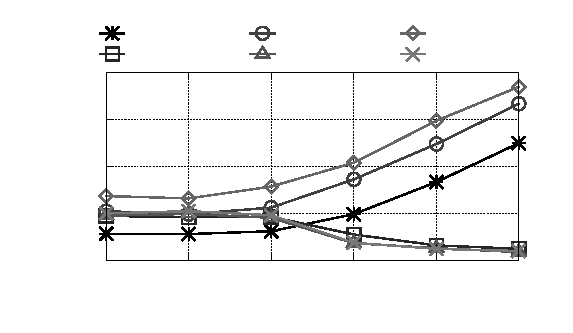
\includegraphics{crime}}%
    \gplfronttext
  \end{picture}%
\endgroup
}
\caption{\Jaccard{\secretsSetSize} for different \secretsSetSize and \roundNmbr}
\label{fig:crime:Jaccard}
\end{subfigure}\\
\begin{tabular}{c}
\begin{subfigure}[b]{1.0\textwidth}
\centering
{\small	
\renewcommand{\arraystretch}{0.96}
\begin{tabular}{lcccccc}
\toprule
\multirow{2}{*}{Procedure}& \multicolumn{3}{c}{\logSecretsSetSizeMinRand{}}& \multicolumn{3}{c}{\logSecretsSetSizeMaxRand}\\ \cline{2-7}
& $\roundNmbr=1$ & $\roundNmbr=2$ & $\roundNmbr=3$ & $\roundNmbr=1$ & $\roundNmbr=2$ & $\roundNmbr=3$\\
\midrule
\renewcommand{\arraystretch}{0.98}
\DTLforeach{crimeresult1}{\m=Column1,\nminone=Column2,\nmintwo=Column3,\nminthree=Column4}{
\DTLforeach[\DTLiseq{\mm}{\m}]{crimeresult2}{\mm=Column1,\nmaxone=Column2,\nmaxtwo=Column3,\nmaxthree=Column4}{ \\[-\normalbaselineskip]
\ifthenelse{\DTLiseq{\m}{$smaz$}}{\smaz & \nminone & \nmintwo & \nminthree & \nmaxone & \nmaxtwo & \nmaxthree \\}{\gzip &\nminone&\nmintwo& \nminthree& \nmaxone& \nmaxtwo &\nmaxthree \\}
}
}
\DTLforeach{crimeresulthex1}{\m=Column1,\nminone=Column2,\nmintwo=Column3,\nminthree=Column4}{
\DTLforeach[\DTLiseq{\mm}{\m}]{crimeresulthex2}{\mm=Column1,\nmaxone=Column2,\nmaxtwo=Column3,\nmaxthree=Column4}{ \\[-\normalbaselineskip]
\iffalse
\ifthenelse{\DTLiseq{\m}{$smaz$}}{\smaz(hex) & \nminone & \nmintwo & \nminthree & \nmaxone & \nmaxtwo & \nmaxthree \\}{\gzip(hex) &\nminone&\nmintwo& \nminthree& \nmaxone& \nmaxtwo &\nmaxthree \\}
\fi
}
}
\\[-\normalbaselineskip]
\bottomrule
\end{tabular}
}
\caption{\secretsSetSizeMaxRand{} and  \secretsSetSizeMaxRand{} for different \roundNmbr}
\label{fig:crime:tbl}
\end{subfigure}
\end{tabular}
\caption{Leakage from \gzip and \smaz (see \secref{sscf:sec:case-studies:crime})}
\label{fig:crime}
\end{figure*}
Our methodology is powerful in accounting for attacker-controlled
inputs, and in this section we demonstrate the benefits of this
capability by applying it to detect \crime
attacks~\cite{Kelsey:2002:CIL:647937.741226,Alawatugoda2015}.  A
\crime vulnerability arises when a web client applies ``unsafe''
compression prior to transmitting a request over TLS.  HTTP requests
can carry information (e.g., the URL parameters) that an attacker can
induce; e.g., if the client visits an attacker-controlled website,
then the attacker can induce requests from the client to another,
target website with URL parameters that the attacker sets.  By
observing the lengths of compressed requests to the target website,
the attacker can deduce whether the attacker-controlled input shares a
substring with a secret contained in the request (e.g., the client's
cookie for the target website) that the attacker is unable to observe
directly.  To be concrete, if the attacker-induced request to the
target website is \url{http://target.com?username=}\textit{name} then
the request will compress better if \textit{name} is a prefix of the
client's cookie for target.com.

\crime attacks utilize the property of an adaptive compression
algorithm that the encoding dictionary is dependent on both the secret
and attacker-controlled variables.  As suggested by Alawatugoda et
al.~\cite{Alawatugoda2015}, a possible mitigation is to separate the
compression for the secret and the other parts of the plaintext or to
use a fixed-dictionary compression algorithm such as
\smaz~\cite{smaz}.  The latter mitigation, though an improvement,
removes the influence of the attacker-controlled input only on the
compression dictionary.  Consider a two-byte plaintext $ab$ whose
first character is secret.  If $a$ is `\texttt{a}', then this two-byte
word will be compressed if $b$ is `\texttt{t}' and will be left
unchanged if $b$ is `\texttt{y}', assuming `\texttt{at}' is in the
dictionary but `\texttt{ay}' is not.  Thus, the leakage should not
be zero even if a fixed-dictionary algorithm is used.

To analyze this scenario in our framework, we modeled the input for
\gzip and \smaz to be of the form
{\small
\begin{tabbing}
  * \= \kill
  \> `\texttt{http://target.com/?} \= \texttt{secret=}' +
  $\SecFn{}(\secretVar)$ + $\AIIFn{}(\textrm{`suffix'})$ 
   + `\texttt{,username=secret=}' + $\ACIFn{}(\textrm{`input'})$
\end{tabbing}
}
\noindent
where `+' denotes concatenation.  Here, $\SecFn{}(\secretVar)$ and
$\ACIFn{}(\textrm{`input'})$ were each one byte,
$\AIIFn{}(\textrm{`suffix'})$ was two bytes, and the
attacker-observable variable was the length of the compressed string.
Each byte was allowed to range over `a', $\ldots$, `z' and
`0',$\ldots$,`9'.  The $\SecFn{}(\secretVar)$ byte after the first
`\texttt{secret=}' plays an analogous role to the client cookie in a
\crime attack, i.e., as the secret to be guessed by the attacker, and
the `\texttt{secret=}' immediately following `\texttt{username=}'
serves as a prefix to match the first instance of `\texttt{secret=}.'


We applied our tool to analyze the leakage susceptibility of
\gzip-1.2.4 and \smaz in this configuration, executed up to three
times ($\roundNmbr \in \{1, 2, 3\}$) with the same secret.  Our
results are shown in \figref{fig:crime}.  Our results show that for
one execution ($\roundNmbr=1$), \smaz is no better than \gzip.  That
is, \secretsSetSizeMax{} and \secretsSetSizeMax{} in
\figref{fig:crime:tbl} suggests that \smaz leaks less information
about some secrets but some information about more secret values
versus \gzip; as mentioned above, \smaz can leak information about a
secret value if it composes a word in its dictionary, as well.
However, the strength of \smaz is revealed as \roundNmbr grows, since
its leakage remains unchanged. In contrast, the leakage of \gzip grows
with \roundNmbr, essentially matching that of \smaz at $\roundNmbr=2$
and surpassing it at $\roundNmbr=3$ (in terms of
\secretsSetSizeMin{}).  This occurs because in each execution of
\gzip, the attacker has the latitude to select a different value for
$\ACIFn{}(\textrm{`input'})$ and then observe that selection's impact
on the length of the compressed string (which in general will change).
In contrast, the leakage of \smaz is independent of the adversary's
choice for $\ACIFn{}(\textrm{`input'})$, and so additional executions
do not leak any additional information.
\iffalse
\zz{Another implicit factor
  impacting the leakage is the inputs domain or the dictionary used in
  the compression.  If limiting the range of inputs to `a', $\ldots$,
  `f', and `0', $\ldots$, `9', instead of all alphanumeric codes,
  \smaz starts to reveals lower leakage than \gzip at $\roundNmbr=1$,
  as the rows for `\gzip(hex)' and `\smaz(hex)' indicate}
\mkr{Why do we consider this case?  And why is it happening?}
\fi

As discussed at the end of \secref{sscf:sec:impl:hash}, a side
effect of our methodology is identifying some example $\langle
\ACIFn{}, \AOOFn{} \rangle$ pairs that lie in
$\possibleDoubles{\secretsSet{}} \setminus \possibleDoubles{\secretsSetAlt{}}$
or $\possibleDoubles{\secretsSetAlt{}} \setminus
\possibleDoubles{\secretsSet{}}$ for samples \secretsSet{},
\secretsSetAlt{} of secrets, which can help in diagnosing a leak.
For example in \tabref{tab:crime:counterexample}, for \gzip in the
$\roundNmbr=1$ case, our tool identified the $\langle \ACIFn{},
\AOOFn{} \rangle$ pair with $\ACIFn{}(\textrm{`input'}) =
\textrm{`c'}$ and $\AOOFn{}(\textrm{`length'}) = 66$ as being in
$\possibleDoubles{\secretsSet{}} \setminus \possibleDoubles{\secretsSetAlt{}}$
for a sampled \secretsSet{}, \secretsSetAlt{} where $\secretsSet{} \ni
\textrm{`c'} = \SecFn{}(\secretVar)$ and $\AIIFn{}(\textrm{`suffix'})
= \textrm{`oo'}$.\footnote{The output length of 66 exceeds the length
  of the input string because \gzip adds a header to the output.
  \smaz attaches no such header.}  As such, the developer now knows
that this $\langle \ACIFn{}, \AOOFn{} \rangle$ pair is consistent with
no secret in \secretsSetAlt{}.  Similarly, for \smaz our tool
identified the pair $\langle \ACIFn{}, \AOOFn{} \rangle$ with
$\ACIFn{}(\textrm{`input'}) = \textrm{`r'}$ and
$\AOOFn{}(\textrm{`length'}) = 36$ as being in
$\possibleDoubles{\secretsSet{}} \setminus \possibleDoubles{\secretsSetAlt{}}$
for a sampled \secretsSet{}, \secretsSetAlt{} where $\secretsSet{} \ni
\textrm{`f'} = \SecFn{}(\secretVar)$ and $\AIIFn{}(\textrm{`suffix'})
= \textrm{`or'}$.
\begin{table}[tbh]
\centering
{\small	
\renewcommand{\arraystretch}{0.98}
\setlength\tabcolsep{0.6ex}
\caption{Examples from $\possibleDoubles{\secretsSet{}} \setminus
    \possibleDoubles{\secretsSetAlt{}}$ for samples \secretsSet{},
    \secretsSetAlt{} ($\roundNmbr=1$) in \crime attacks\label{tab:crime:counterexample}}
\begin{tabular}{ lccccc }
      \toprule
&  &  $\ACIFn{}(\textrm{`input'})$ & $\AOOFn{}(\textrm{`length'})$ & \SecFn{}(\secretVar) & $\AIIFn{}(\textrm{`suffix'})$ \\
\midrule
\gzip & & `c'& 66& `c'  & `oo'\\
\smaz & & `r' & 36 & `f' & `or' \\
\bottomrule
\end{tabular}
}
\end{table}

\newcommand{\tcpmib}{\texttt{tcp\_mib}\xspace}
\newcommand{\linuxmib}{\texttt{linux\_mib}\xspace}
\newcommand{\tcprcvfunc}{\texttt{tcp\_rcv\_established}\xspace}
\newcommand{\tcpparseoption}{\texttt{tcp\_parse\_options}\xspace}
\newcommand{\sk}{\texttt{sk}\xspace}
\newcommand{\skb}{\texttt{skb}\xspace}
\newcommand{\tcphdr}{\texttt{th}\xspace}
\newcommand{\len}{\texttt{len}\xspace}
\newcommand{\tcpseq}{\texttt{tp->rcv\_nxt}\xspace}
\newcommand{\tcpack}{\texttt{tp->snd\_nxt}\xspace}
\newcommand{\tcprcvwnd}{\texttt{tp->rcv\_wnd}\xspace}
\newcommand{\tcpsndwnd}{\texttt{tp->snd\_wnd}\xspace}
\newcommand{\skbseq}{\texttt{TCP\_SKB\_CB(skb)->seq}\xspace}
\newcommand{\skbendseq}{\texttt{TCP\_SKB\_CB(skb)->end\_seq}\xspace}
\newcommand{\skback}{\texttt{TCP\_SKB\_CB(skb)->ack\_seq}\xspace}
\newcommand{\tcpflagword}{\texttt{tcp\_flag\_word(th)}\xspace}
\newcommand{\maxtcpwnd}{\texttt{MAX\_TCP\_WINDOW}\xspace}
\newcommand{\fillpkg}{\texttt{fill\_packet}\xspace}
\newcommand{\tcpinitsock}{\texttt{tcp\_init\_sock}\xspace}
\newcommand{\netincstatsbh}{\texttt{NET\_INC\_STATS\_BH}\xspace}
\newcommand{\linuxmibdelayedacklost}{\texttt{LINUX\_MIB\_DELAYEDACKLOST}\xspace}

\subsection{Linux TCP sequence number leakage}
\label{sscf:sec:case-studies:tcp}

Known side channels in some TCP implementations leak TCP sequence and
acknowledgment numbers~\cite{tcp:1985,Qian:2012:CTS}.  In some cases,
these side channels can be used by off-path attackers to terminate or
inject malicious payload into
connections~\cite{zhiyun:2016,Qian:2012:CTS}.  The origin of these
attacks is shared network counters (e.g., \linuxmib and \tcpmib) that
are used to record connection statistics across different connections
in the same network namespace.

These counters have been implicated in numerous side channels since
version 2.0 of the Linux kernel~\cite{tcp:1999}.  For example, the
code snippet (without the patch in
\linerefs{line:patchstart}{line:patchend}) in \figref{fig:leak} leaks
the secret \tcpseq in Linux-3.18 TCP.  Here, the attacker controls the
\skb input and so the value \skbseq that is compared to \tcpseq on
\lineref{line:leak}.  Based on this comparison, the \netincstatsbh
procedure increments an attacker-observable counter indicated by
\linuxmibdelayedacklost (\lineref{line:signalend}).
If the attacker can repeatedly cause the procedure in
\figref{fig:leak} to be invoked with inputs \skb of its choice, it can
use binary search to infer \tcpseq within 32
executions~\cite{Qian:2012:CTS}.

\lstdefinestyle{customc}{
  belowcaptionskip=1\baselineskip,
  breaklines=true,
  xleftmargin=\parindent,
  language=C,
  showstringspaces=false,
  basicstyle=\scriptsize\ttfamily,
}
\lstset{escapechar=@,style=customc}
\begin{figure}\centering
\begin{minipage}[b]{0.9\linewidth}
\centering
{
\lstset{escapechar=@,style=customc}
 \begin{lstlisting}[language=c,numbers=left,escapechar=^,numberstyle=\small, numbersep=4pt, ] 
void tcp_send_dupack(struct sock *sk,
                     const struct sk_buff *skb) {
 struct tcp_sock *tp = tcp_sk(sk);
 if (TCP_SKB_CB(skb)->end_seq != TCP_SKB_CB(skb)->seq &&
    before(TCP_SKB_CB(skb)->seq, tp->rcv_nxt)) {^\label{line:leak}^
+  if (before(TCP_SKB_CB(skb)->ack_seq, tp->snd_una - tp->max_window) ^\label{line:patchstart}^
+      || after(TCP_SKB_CB(skb)->ack_seq, tp->snd_nxt)) { 
+    tcp_send_ack(sk);
+    return;
+  } ^\label{line:patchend}^
   NET_INC_STATS_BH(sock_net(sk), LINUX_MIB_DELAYEDACKLOST);^\label{line:signalend}^
   ...
 }
 tcp_send_ack(sk);
}
\end{lstlisting}
}
\end{minipage}
\caption[A code snippet for Linux TCP implementation]{A code snippet vulnerable to leaking the TCP sequence number
  in linux 3.18; lines marked `+' indicate a hypothetical patch with
  which we experimented (see \secref{sscf:sec:case-studies:tcp})}
\label{fig:leak}
\end{figure}

The most straightforward mitigation for this leakage is to disable the
public counters.  This will stop the leakage, but will disable some
mechanisms such as audit logging.  Another potential mitigation is to
increase the difficulty of increasing the public counter, by adding
additional checking related to more secret variables. For example,
before increasing the \linuxmibdelayedacklost counter, the procedure
could also check for correct acknowledgment numbers, as shown in the patch in
\linerefs{line:patchstart}{line:patchend}. As far as we know, our
study is the first to compare these potential
mitigations for TCP sequence and acknowledgment number leakage.

To analyze the information leakage in this example, we compiled a
user-mode Linux kernel~\cite{dike2001user} as a library.  Our target
procedure for analysis was \tcprcvfunc, which is of the form
\begin{lstlisting}[language=c,basicstyle=\small\ttfamily,xleftmargin=0pt,xrightmargin=0pt]
void tcp_rcv_established(struct sock *sk,
  struct sk_buff *skb,
  const struct tcphdr *th,
  unsigned int len) {
  struct tcp_sock* tp = (struct tcp_sock*) sk;
  ...
}
\end{lstlisting}%
The inputs for \tcprcvfunc have many constraints among them
when passed in, for instance
\begin{center}
{\small
$\skbseq  < \skbendseq$\\
$\tcprcvwnd  \leq \maxtcpwnd$ \\
$\tcpsndwnd  \leq \maxtcpwnd$
}
\end{center}
To generate constraints for the inputs to \tcprcvfunc, we applied
symbolic execution to the procedures \fillpkg and \tcpinitsock.
Symbolic buffers to represent these inputs and their associated
constraints were then assembled within
\tcprcvfunc.  We also stubbed out several procedure
calls\footnote{Specifically, we stubbed out \texttt{get\_seconds},
  \texttt{current\_thread\_info}, \texttt{tcp\_options\_write},
  \texttt{tcp\_sendmsg}, \texttt{prandom\_bytes},
  \texttt{current\_thread\_info}, \tcpparseoption, and
  \texttt{tcp\_checksum\_complete\_user}.}  within \tcprcvfunc,
causing each to simply return a symbolic buffer so as to avoid
symbolically executing it, since doing so introduced problems for
\klee (e.g., dereferencing symbolic pointers).

After generating the postcondition for the procedure \tcprcvfunc, we
defined the attacker-controlled inputs to be 

\parbox{\linewidth}{
	\small{
\begin{align*}
	\ACIKeys  = \{&\skbseq, \\
	&\skbendseq, \\
	&\skback, \\
	& \tcpflagword\}
\end{align*}
}}
(each four bytes) and the attacker-observable variables to be
$\AOOKeys = \{\linuxmib$, $\tcpmib\}$.  All fields of constrained
input structures (e.g., \texttt{tp->snd\_una} and
\texttt{tp->max\_window}) not covered by \ACIKeys and \AOOKeys were
added to \AIIKeys, with the secret variables\footnote{Though we have
  described our framework so far using one secret variable, it extends
  trivially to more.} being \tcpseq and \tcpack (each four bytes).  We
conducted single-execution ($\roundNmbr=1$, denoted `v3.18-1run'),
two-execution ($\roundNmbr=2$, denoted `v3.18-2run') and
three-execution ($\roundNmbr=3$, denoted `v3.18-3run') leakage
analysis.  In the multi-execution analysis, we assumed \texttt{*\sk} to
be the same in multiple executions
($\AIIFn{1}(\textrm{`}\texttt{*sk}\textrm{'})$ $=$
$\AIIFn{2}(\textrm{`}\texttt{*sk}\textrm{'})$ $=$ $\ldots$ $=$
$\AIIFn{\roundNmbr}(\textrm{`}\texttt{*sk}\textrm{'})$) since its fields
used in \tcprcvfunc would be unchanged or, if changed, would be
changed predictably.

The results from this analysis are shown in \figref{fig:tcp}.  The
inset graph in \figref{fig:tcp:JaccardRand} is a magnification of the
portion of the curve in the interval $[0, 8]$ on the horizontal axis.
Specifically, the highest leakage resulted from `v3.18-3run', followed
by `v3.18-2run' and `v3.18-1run', as indicated by the
\JaccardRand{\secretsSetSize} curves in \figref{fig:tcp:JaccardRand}
and the \secretsSetSizeMinRand{} and \secretsSetSizeMaxRand{} measures in
\figref{fig:tcp:tlb}.  This shows the potential for the attacker to
extract more information about the secrets \tcpseq and \tcpack using
multiple executions.  This is consistent with the observation that a
smart attacker could utilize this side channel to infer one bit per
execution~\cite{Qian:2012:CTS}.

\begin{figure}
\centering
\begin{subfigure}[b]{0.6\linewidth}
  \centering
  \resizebox{0.9\textwidth}{!}{\scriptsize% GNUPLOT: LaTeX picture with Postscript
\begingroup
  \fontfamily{Times-Roman}%
  \selectfont
  \makeatletter
  \providecommand\color[2][]{%
    \GenericError{(gnuplot) \space\space\space\@spaces}{%
      Package color not loaded in conjunction with
      terminal option `colourtext'%
    }{See the gnuplot documentation for explanation.%
    }{Either use 'blacktext' in gnuplot or load the package
      color.sty in LaTeX.}%
    \renewcommand\color[2][]{}%
  }%
  \providecommand\includegraphics[2][]{%
    \GenericError{(gnuplot) \space\space\space\@spaces}{%
      Package graphicx or graphics not loaded%
    }{See the gnuplot documentation for explanation.%
    }{The gnuplot epslatex terminal needs graphicx.sty or graphics.sty.}%
    \renewcommand\includegraphics[2][]{}%
  }%
  \providecommand\rotatebox[2]{#2}%
  \@ifundefined{ifGPcolor}{%
    \newif\ifGPcolor
    \GPcolortrue
  }{}%
  \@ifundefined{ifGPblacktext}{%
    \newif\ifGPblacktext
    \GPblacktexttrue
  }{}%
  % define a \g@addto@macro without @ in the name:
  \let\gplgaddtomacro\g@addto@macro
  % define empty templates for all commands taking text:
  \gdef\gplbacktext{}%
  \gdef\gplfronttext{}%
  \makeatother
  \ifGPblacktext
    % no textcolor at all
    \def\colorrgb#1{}%
    \def\colorgray#1{}%
  \else
    % gray or color?
    \ifGPcolor
      \def\colorrgb#1{\color[rgb]{#1}}%
      \def\colorgray#1{\color[gray]{#1}}%
      \expandafter\def\csname LTw\endcsname{\color{white}}%
      \expandafter\def\csname LTb\endcsname{\color{black}}%
      \expandafter\def\csname LTa\endcsname{\color{black}}%
      \expandafter\def\csname LT0\endcsname{\color[rgb]{1,0,0}}%
      \expandafter\def\csname LT1\endcsname{\color[rgb]{0,1,0}}%
      \expandafter\def\csname LT2\endcsname{\color[rgb]{0,0,1}}%
      \expandafter\def\csname LT3\endcsname{\color[rgb]{1,0,1}}%
      \expandafter\def\csname LT4\endcsname{\color[rgb]{0,1,1}}%
      \expandafter\def\csname LT5\endcsname{\color[rgb]{1,1,0}}%
      \expandafter\def\csname LT6\endcsname{\color[rgb]{0,0,0}}%
      \expandafter\def\csname LT7\endcsname{\color[rgb]{1,0.3,0}}%
      \expandafter\def\csname LT8\endcsname{\color[rgb]{0.5,0.5,0.5}}%
    \else
      % gray
      \def\colorrgb#1{\color{black}}%
      \def\colorgray#1{\color[gray]{#1}}%
      \expandafter\def\csname LTw\endcsname{\color{white}}%
      \expandafter\def\csname LTb\endcsname{\color{black}}%
      \expandafter\def\csname LTa\endcsname{\color{black}}%
      \expandafter\def\csname LT0\endcsname{\color{black}}%
      \expandafter\def\csname LT1\endcsname{\color{black}}%
      \expandafter\def\csname LT2\endcsname{\color{black}}%
      \expandafter\def\csname LT3\endcsname{\color{black}}%
      \expandafter\def\csname LT4\endcsname{\color{black}}%
      \expandafter\def\csname LT5\endcsname{\color{black}}%
      \expandafter\def\csname LT6\endcsname{\color{black}}%
      \expandafter\def\csname LT7\endcsname{\color{black}}%
      \expandafter\def\csname LT8\endcsname{\color{black}}%
    \fi
  \fi
    \setlength{\unitlength}{0.0500bp}%
    \ifx\gptboxheight\undefined%
      \newlength{\gptboxheight}%
      \newlength{\gptboxwidth}%
      \newsavebox{\gptboxtext}%
    \fi%
    \setlength{\fboxrule}{0.5pt}%
    \setlength{\fboxsep}{1pt}%
\begin{picture}(4896.00,3024.00)%
    \gplgaddtomacro\gplbacktext{%
      \csname LTb\endcsname%
      \put(490,456){\makebox(0,0)[r]{\strut{}$0$}}%
      \csname LTb\endcsname%
      \put(490,970){\makebox(0,0)[r]{\strut{}$0.2$}}%
      \csname LTb\endcsname%
      \put(490,1483){\makebox(0,0)[r]{\strut{}$0.4$}}%
      \csname LTb\endcsname%
      \put(490,1997){\makebox(0,0)[r]{\strut{}$0.6$}}%
      \csname LTb\endcsname%
      \put(490,2510){\makebox(0,0)[r]{\strut{}$0.8$}}%
      \csname LTb\endcsname%
      \put(570,266){\makebox(0,0){\strut{}$0$}}%
      \csname LTb\endcsname%
      \put(1111,266){\makebox(0,0){\strut{}$8$}}%
      \csname LTb\endcsname%
      \put(1651,266){\makebox(0,0){\strut{}$16$}}%
      \csname LTb\endcsname%
      \put(2192,266){\makebox(0,0){\strut{}$24$}}%
      \csname LTb\endcsname%
      \put(2733,266){\makebox(0,0){\strut{}$32$}}%
      \csname LTb\endcsname%
      \put(3273,266){\makebox(0,0){\strut{}$40$}}%
      \csname LTb\endcsname%
      \put(3814,266){\makebox(0,0){\strut{}$48$}}%
      \csname LTb\endcsname%
      \put(4354,266){\makebox(0,0){\strut{}$56$}}%
      \csname LTb\endcsname%
      \put(4895,266){\makebox(0,0){\strut{}$64$}}%
    }%
    \gplgaddtomacro\gplfronttext{%
      \csname LTb\endcsname%
      \put(19,1502){\rotatebox{-270}{\makebox(0,0){\strut{}\JaccardRand{\secretsSetSize}}}}%
      \put(2732,95){\makebox(0,0){\strut{}$\log_2{\secretsSetSize}$}}%
      \csname LTb\endcsname%
      \put(877,2866){\makebox(0,0)[l]{\strut{}v3.18-1run}}%
      \csname LTb\endcsname%
      \put(877,2676){\makebox(0,0)[l]{\strut{}v3.18-patched}}%
      \csname LTb\endcsname%
      \put(2422,2866){\makebox(0,0)[l]{\strut{}v3.18-2run}}%
      \csname LTb\endcsname%
      \put(3450,2676){\makebox(0,0)[l]{\strut{}v3.18-rmCounter}}%
      \csname LTb\endcsname%
      \put(3967,2866){\makebox(0,0)[l]{\strut{}v3.18-3run}}%
    }%
    \gplgaddtomacro\gplbacktext{%
      \csname LTb\endcsname%
      \put(1121,907){\makebox(0,0)[r]{\strut{}0}}%
      \put(1121,1310){\makebox(0,0)[r]{\strut{}0.2}}%
      \put(1121,1713){\makebox(0,0)[r]{\strut{}0.4}}%
      \put(1121,2116){\makebox(0,0)[r]{\strut{}0.6}}%
      \put(1224,770){\makebox(0,0){\strut{}0}}%
      \put(1591,770){\makebox(0,0){\strut{}1}}%
      \put(1958,770){\makebox(0,0){\strut{}2}}%
      \put(2325,770){\makebox(0,0){\strut{}3}}%
      \put(2692,770){\makebox(0,0){\strut{}4}}%
      \put(3059,770){\makebox(0,0){\strut{}5}}%
      \put(3426,770){\makebox(0,0){\strut{}6}}%
      \put(3793,770){\makebox(0,0){\strut{}7}}%
      \put(4160,770){\makebox(0,0){\strut{}8}}%
    }%
    \gplgaddtomacro\gplfronttext{%
    }%
    \gplbacktext
    \put(0,0){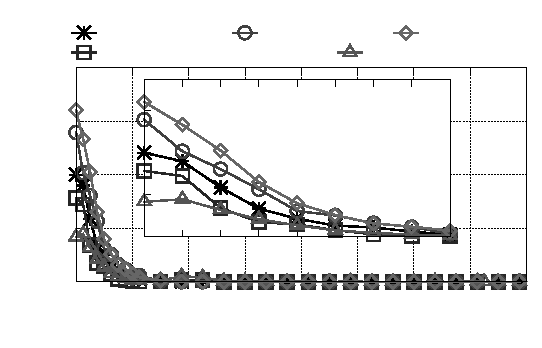
\includegraphics{linux-other}}%
    \gplfronttext
  \end{picture}%
\endgroup
}
\caption{\JaccardRand{\secretsSetSize} per \secretsSetSize and version of \tcprcvfunc \label{fig:tcp:JaccardRand}}
\end{subfigure}
\hspace{-2ex}
\begin{subfigure}[b]{0.34\linewidth}
\vspace{1ex}
  \small{
  \centering
	\DTLloaddb[noheader=true,headers={Procedure,\logSecretsSetSizeMin,\logSecretsSetSizeMax}]{linuxresult}{fig/sscf/linux-0.csv}
	\DTLloaddb[noheader=true,headers={Procedure,\logSecretsSetSizeMin,\logSecretsSetSizeMax}]{linuxother}{fig/sscf/linux-other-0.csv}
	\setlength\tabcolsep{0.7ex}
	%\drawTblTwo{version}{linuxresult}{linuxother}
	\begin{tabular}{lcc}\toprule
Version & {\logSecretsSetSizeMinRand}& {\logSecretsSetSizeMaxRand}\\ 
\midrule
\DTLforeach{linuxother}{\m=Column1,\nmin=Column2,\nmax=Column3}{\m & \nmin & \nmax \tabularnewline}
\\[-\normalbaselineskip]\bottomrule
\end{tabular}
}
\vspace{7ex}
 %\drawTbl{version}{linuxother}
\caption{\secretsSetSizeMinRand{} and \secretsSetSizeMaxRand{} for versions of \tcprcvfunc \label{fig:tcp:tlb}}
\end{subfigure}
\caption{TCP sequence-number leakage (see \secref{sscf:sec:case-studies:tcp})}
\label{fig:tcp}
\end{figure}

To alleviate this leak, we applied a hypothetical patch shown
in \figref{fig:leak} that checks another secret value \tcpack before
incrementing the counter for \linuxmibdelayedacklost.  Our analysis
results (for $\roundNmbr=1$ execution, denoted `v3.18-patched') in
\figref{fig:tcp} shows that the patch alleviated the leakage somewhat.
We also tried just deleting \lineref{line:leak}-\ref{line:signalend}
from the original (unpatched) code in \figref{fig:leak}.  As shown in
\figref{fig:tcp}, this version (denoted `v3.18-rmCounter') evidently
has lower leakage than `v3.18-patched'.  In considering these
mitigations, we stress that our patch addressed only the leakage
arising from \lineref{line:leak}, and not all sources that leak
information about \tcpseq or \tcpack (which are numerous, see Chen et
al.~\cite{Chen:static}).  Our results suggest, however, that our
methodology could guide developers in mitigating leaks in their code.

\subsection{Performance}
\label{sscf:sec:case-studies:perf}

Performance of our tool involves two major components, namely the time
to compute the postcondition \postcondition{\proc}{} via symbolic
execution, and the time to calculate \Jaccard{\secretsSetSize} or
\JaccardRand{\secretsSetSize} for different \secretsSetSize starting
from \postcondition{\proc}{}.  Postcondition generation is not a topic
in which we innovate, and so we defer discussion of its costs in our
case studies to \secref{sscf:sec:symbolic}.  Here we focus on the costs of
calculating \Jaccard{\secretsSetSize} or \JaccardRand{\secretsSetSize}
for different \secretsSetSize starting from \postcondition{\proc}{}.

%\subsubsection{Computation of \Jaccard{\secretsSetSize} and \JaccardRand{\secretsSetSize}}
%\label{sscf:sec:case-studies:perf:counting}

Starting from \postcondition{\proc}{}, the
computation of \Jaccard{\secretsSetSize} or
\JaccardRand{\secretsSetSize} can be parallelized almost arbitrarily.
Not only can \Jaccard{\secretsSetSize} or
\JaccardRand{\secretsSetSize} for each \secretsSetSize be computed
independently, but even for a single value of \secretsSetSize, the
estimation of $\Jaccard{}(\secretsSet{}, \secretsSetAlt{})$ or
$\JaccardRand{}(\secretsSet{}, \secretsSetAlt{})$ can be computed for
each pair of sampled sets \secretsSet{}, \secretsSetAlt{} and each
estimation iteration independently.  In \figref{fig:micro-cal}, we
report the \textit{average} estimation time per sample pair, which indicates
that all case studies could finish one estimation
in~\eqref{eqn:possibleDoublesEstimate} for one sample pair within
about one minute.  As such, the speed of calculating final pair
\secretsSetSizeMin{} and \secretsSetSizeMax{} is limited primarily by
the number of processors available for the computation.

\begin{figure}
  \centering
  \small
  		\setlength\tabcolsep{0.6ex}
    \begin{tabular}{clcccc}
      \toprule
      \textbf{Sec.} & \textbf{Procedure} & $\Jaccard{}(\secretsSet{},
\secretsSetAlt{})$ & $\JaccardRand{}(\secretsSet{},
\secretsSetAlt{})$ & $\Jaccard{\secretsSetSize{}}$& $\JaccardRand{\secretsSetSize{}}$ \\
      \midrule
       \ref{sscf:sec:case-studies:sphinx} & Auto-complete (nopadding) &
	   34\millisecs & 56\millisecs\ & 5\mins & 7\mins\\
        \ref{sscf:sec:case-studies:sphinx} & Auto-complete (fix.64) &
		48\millisecs &  65\millisecs & 6\mins & 8\mins\\
        \ref{sscf:sec:case-studies:sphinx} & Auto-complete (fix.256) &
		43\millisecs & 57\millisecs & 6\mins & 7\mins\\
      \ref{sscf:sec:case-studies:sphinx} & Auto-complete (rand.64)& & 1.2\secs & & 15\mins\\
      \ref{sscf:sec:case-studies:crime} & \gzip &  &  26\secs &  & 4\hours \\
      \ref{sscf:sec:case-studies:crime} & \smaz &  &  40\secs &  & 10\hours  \\
      \ref{sscf:sec:case-studies:tcp} & v3.18-1run  &  & 73\secs & & 20\hours\\ 
      \ref{sscf:sec:case-studies:tcp} & v3.18-patched &  & 67\secs & & 20\hours \\
      \ref{sscf:sec:case-studies:tcp} & v3.18-rmCounter &  & 50\secs &  & 19\hours \\
      \bottomrule
    \end{tabular}
  \caption{Average time per estimate ($\Jaccard{}(\secretsSet{},
    \secretsSetAlt{})$ or $\JaccardRand{}(\secretsSet{},
    \secretsSetAlt{})$) and most expensive overall time
    ($\Jaccard{\secretsSetSize{}}$ or
    $\JaccardRand{\secretsSetSize{}}$) for case studies}
  \label{fig:micro-cal}
\end{figure}

In our experiments, performed on a DELL PowerEdge R815 server with
2.3\gigahertz AMD Opteron 6376 processors and 128\gigabytes memory, we
computed \Jaccard{\secretsSetSize} or \JaccardRand{\secretsSetSize}
per value of \secretsSetSize on its own core.  As reported in the last
two columns of \figref{fig:micro-cal}, the time to do so for the
\textit{most expensive} value of \secretsSetSize ranged from roughly
15m for the auto-complete procedure of
\secref{sscf:sec:case-studies:sphinx} to about 20h for the Linux TCP
implementations of \secref{sscf:sec:case-studies:tcp}.  For several of our
case studies (see \figref{fig:micro-cal}), we experimented with
calculating \JaccardRand{\secretsSetSize} even when
\Jaccard{\secretsSetSize} was sufficient, and found its estimation to
cost $\le2\times$ that of estimating \Jaccard{\secretsSetSize}, due to
the duplication of \postcondition{\proc}{} in
\possibleTriplesIntersectByPrefix{\hashFnOutputPrefix}.

%\subsubsection{Implications}
%\label{sscf:sec:case-studies:performance:implications}

To place the above numbers in some context, the $\approx$ 20h (for the
worst \secretsSetSize, without parallelization) dedicated to computing
a value of \Jaccard{\secretsSetSize} in the Linux TCP case study of
\secref{sscf:sec:case-studies:tcp} involved a procedure \proc of which 165
bytes of its inputs were somehow used in the procedure.  A naive
alternative to our design in which all possible inputs are enumerated
and run through the procedure to compute its outputs (and interference
measured from these input-output pairs, perhaps as we do) would
therefore involve enumerating $2^{1320}$ possible inputs, which is
obviously impractical.

In this light, our technique that performs interference analysis for
real codebases in the timeframe of minutes-to-hours (and far faster
with parallelization) is a dramatic improvement.  Moreover, these
results are likely to only improve with advances in symbolic execution
and model counting.  Even our experimentation with various
optimizations for postcondition generation and model counting was not
exhaustive.  That said, the results above suggest that the costs of
our approach are likely to remain sufficiently high for real codebases
to preclude its use for interactive analysis by human programmers.
Rather, we expect that our analysis could be run as a diagnostic
technique overnight, for example.

\section{Discussion and Limitations}
\label{sscf:sec:discussion}
The static method to quantify noninterference builds from two tasks
that are recognized, difficult challenges in computer science.  The
first is the construction of a logical postcondition
\postcondition{\proc}{} for a procedure \proc, for which we leverage
symbolic execution.  As such, our technique inherits the limitations
of existing symbolic execution tools and those incumbent on generating
postconditions, more generally.  For example, symbolic execution is
difficult to scale to some procedures, and challenges involving
symbolic pointers and unbounded loops can require workarounds, as they
did in our TCP case study (\secref{sscf:sec:case-studies:tcp}).  The second
challenge problem underpinning our methodology is model counting,
which is \#P-complete. We are optimistic that future improvements in
these areas will be amenable to adoption within our methodology. While
the resulting tool is not yet quick enough to support interactive use,
it is positioned to benefit from advances in symbolic execution and
approximate model counting, both active areas of research.

Our approach is powerful in that it can be applied to scenarios in
which the distributions of inputs---whether they be attacker
controlled or other---are unknown, and this is often the case in
practice.  In some cases, the input distributions are unknowable,
especially for \ACIKeys.  In others, they may be knowable but require
considerable empirical data to estimate (e.g., the distributions of
user-input search terms, in a context like that of
\secref{sscf:sec:case-studies:sphinx}).  That said, because it is
insensitive to these distributions, it does not offer an immediate way
to accommodate these distributions if they are known.  Still, our
methodology allows these inputs to be accounted for in a principled
way, in contrast to others that either disallow them or assign them
heuristically.

Our measure does not take into account computational limits on the
attacker, as is typically assumed by cryptographic algorithms.  As
such, our measure is best viewed as a measure of information-theoretic
security, where the attacker has unlimited computation power.  For
example, assuming it were possible to generate our measure for a
digital signature algorithm, our measure would typically indicate that
a signature and public key divulges the private key, even if the
private key is intractable to compute.  That said, due to hardness in
solving a cryptographic problem with a solver, secrets hidden by
cryptography would typically be intractable to generate postconditions
for.

\section{Summary}
\label{sscf:sec:summary}

In this chapter we have suggested a static method for assessing
interference and attempts to mitigate it.  Informally,
noninterference is achieved when the output produced by a procedure in
response to an adversary's input is unaffected by secret values that
the adversary is not authorized to observe.  Following this intuition,
we have developed an automatic tool to estimate the number of pairs of
attacker-controlled inputs and attacker-observable outputs that are
possible, conditioned on the secret being limited to a particular
sample.  The discovery of such pairs that are possible for one sample
but not another reveals interference.

We clarified the effectiveness of our strategy both on artificial
examples (\secref{sscf:sec:micro}) and on real-world codebases
(\secref{sscf:sec:case-studies}).  Specifically, we evaluated leakage in
the \sphinx auto-complete feature of its search interface due to its
response sizes, and the effectiveness of a variety of mitigations
(\secref{sscf:sec:case-studies:sphinx}); the \crime vulnerabilities of
adaptive compression in \gzip and fixed-dictionary compression in
\smaz (\secref{sscf:sec:case-studies:crime}); and leakage of TCP sequence
numbers in Linux and the effectiveness of two mitigations of our own
design (\secref{sscf:sec:case-studies:tcp}).  Within these contexts we also
explored leakage over a single procedure execution and over many, and
showed that our framework allowed for a useful comparison of how
procedures leaked data as the number of executions grows.

Central to our methodology's ability to scale to real codebases is our
expression of leakage assessment within a framework that permits the
use of approximate model counting (and specifically hash-based model
counting). 






